\section{Metadata}

\begin{landscape}

\subsection{sysdiagrams}

\subsubsection{Table Overview}
\begin{itemize}
\item \textbf{Table Name:} sysdiagrams
\item \textbf{Schema:} dbo
\item \textbf{Number of Records:} 0
\item \textbf{Number of Columns:} 5
\end{itemize}

\subsubsection{Column Details}
\begin{longtable}{|l|l|l|r|p{6cm}|}
\hline
\textbf{Column Name} & \textbf{Data Type} & \textbf{Description} & \textbf{N} & \textbf{Statistics/Values} \\
\hline
\endfirsthead
\multicolumn{5}{c}{\textit{Continued from previous page}} \\
\hline
\textbf{Column Name} & \textbf{Data Type} & \textbf{Description} & \textbf{N} & \textbf{Statistics/Values} \\
\hline
\endhead
\hline
\multicolumn{5}{c}{\textit{Continued on next page}} \\
\endfoot
\hline
\endlastfoot
name & nvarchar(128) &  & 0 & All NULL values \\
\hline
principal\_id & int(10) &  & 0 & All NULL values \\
\hline
diagram\_id & int(10) &  & 0 & All NULL values \\
\hline
version & int(10) &  & 0 & All NULL values \\
\hline
definition & varbinary(-1) &  & 0 & All NULL values \\
\hline
\end{longtable}

\subsection{tbl\_Budgets}

\subsubsection{Table Overview}
\begin{itemize}
\item \textbf{Table Name:} tbl\_Budgets
\item \textbf{Schema:} dbo
\item \textbf{Number of Records:} 219,457
\item \textbf{Number of Columns:} 19
\end{itemize}

\subsubsection{Column Details}
\begin{longtable}{|l|l|l|r|p{6cm}|}
\hline
\textbf{Column Name} & \textbf{Data Type} & \textbf{Description} & \textbf{N} & \textbf{Statistics/Values} \\
\hline
\endfirsthead
\multicolumn{5}{c}{\textit{Continued from previous page}} \\
\hline
\textbf{Column Name} & \textbf{Data Type} & \textbf{Description} & \textbf{N} & \textbf{Statistics/Values} \\
\hline
\endhead
\hline
\multicolumn{5}{c}{\textit{Continued on next page}} \\
\endfoot
\hline
\endlastfoot
CaseNo & bigint(19) & Consumer iConnect ID & 42093 & Range: [10184.00, 100198.00], Avg: 39353.87, Median: 35849.00 \\
\hline
BudgetID & bigint(19) & Budget ID & 219457 & Range: [66.00, 219554.00], Avg: 109819.48, Median: 109821.00 \\
\hline
BudgetType & varchar(100) & Budget Type & 2 & \{CDC+, iBudget\} \\
\hline
BudgetStatus & varchar(100) & Budget Status & 4 & \{Approved, Budget Approved, Draft, Terminated\} \\
\hline
FiscalYear & varchar(100) & FiscalYear & 6 & \{2021, 2022, 2023, 2024, 2025, 2026\} \\
\hline
Programs & varchar(75) & Program Consumer Enrolled into & 2 & \{APD Waiver, CDC+\} \\
\hline
WSC & varchar(100) & Waiver Support Coordinator Name & 1031 & ... \\
\hline
ApprovedBy & int(10) & Approved By APD Staff Name & 6 & Range: [1182.00, 34038.00], Avg: 9428.56, Median: 2487.00 \\
\hline
ApprovalDate & datetime & Approval Date & 15 & Range: [2020-05-22, 2025-05-21] \\
\hline
StartDate & datetime & Start Date & 271 & Range: [2020-07-01, 2025-07-22] \\
\hline
EndDate & datetime & End Date & 6 & Range: [2021-06-30, 2026-06-30] \\
\hline
BudgetAmount & numeric(19,2) & Budget Amount & 146839 & Range: [-28280.29, 894542.33], Avg: 58144.60, Median: 49936.11 \\
\hline
AnnualizedAmount & numeric(19,2) & Annualized Budget Amount & 131128 & Range: [-54617.64, 485174942.72], Avg: 61506.63, Median: 51322.04 \\
\hline
AmountEncumbered & numeric(19,2) & Amount Encumbered & 147533 & Range: [0.00, 1236377.20], Avg: 50557.89, Median: 41775.08 \\
\hline
AmountUnauthorized & numeric(19,2) & Amount Unauthorized & 121870 & Range: [-1073148.93, 850693.76], Avg: 9621.87, Median: 1882.51 \\
\hline
PrioriBudgetAmount & numeric(19,2) & Priori Budget Amount & 150649 & Range: [0.00, 1144471.65], Avg: 52194.31, Median: 43875.48 \\
\hline
Comments & varchar(-1) & Comments & 121 & ... \\
\hline
UserStamp & varchar(100) & UserStamp & 61 & ... \\
\hline
DateTimeStamp & datetime & DateTimeStamp & 49148 & Range: [2020-05-25, 2025-09-11] \\
\hline
\end{longtable}

\subsection{tbl\_Claims\_MMIS}

\subsubsection{Table Overview}
\begin{itemize}
\item \textbf{Table Name:} tbl\_Claims\_MMIS
\item \textbf{Schema:} dbo
\item \textbf{Number of Records:} 37,750,736
\item \textbf{Number of Columns:} 20
\end{itemize}

\subsubsection{Column Details}
\begin{longtable}{|l|l|l|r|p{6cm}|}
\hline
\textbf{Column Name} & \textbf{Data Type} & \textbf{Description} & \textbf{N} & \textbf{Statistics/Values} \\
\hline
\endfirsthead
\multicolumn{5}{c}{\textit{Continued from previous page}} \\
\hline
\textbf{Column Name} & \textbf{Data Type} & \textbf{Description} & \textbf{N} & \textbf{Statistics/Values} \\
\hline
\endhead
\hline
\multicolumn{5}{c}{\textit{Continued on next page}} \\
\endfoot
\hline
\endlastfoot
CaseNo & bigint(19) & Consumer iConnect ID & 41285 & Range: [10184.00, 99376.00], Avg: 36590.87, Median: 33566.00 \\
\hline
PIN & varchar(20) & Legacy ABC PIN & 41267 & ... \\
\hline
ProviderName & varchar(500) & Provider Name & 5249 & ... \\
\hline
ProviderMedcId & varchar(20) & Provider Medicaid ID & 5004 & ... \\
\hline
ProcCode & varchar(20) & Service Procedure Code & 156 & ... \\
\hline
ServiceDate & datetime & Date Service Provided & 1886 & Range: [2020-07-01, 2025-08-29] \\
\hline
Units & int(10) & Units & 1958 & Range: [-98112.00, 98112.00], Avg: 17.94, Median: 15.00 \\
\hline
BilledAmt & numeric(9,2) & Billed Amount & 47855 & Range: [-25270.05, 36622.37], Avg: 191.90, Median: 101.40 \\
\hline
PaidAmt & numeric(9,2) & Paid Amount & 46066 & Range: [-21173.51, 26975.48], Avg: 191.69, Median: 101.40 \\
\hline
PaidDate & datetime & Paid Date & 541 & Range: [2020-07-03, 2025-09-03] \\
\hline
ICN & varchar(100) & ICN - Claim Number in FMMIS & 11172269 & ... \\
\hline
AdjustICN & varchar(100) & AdjustICN & 407203 & ... \\
\hline
TreatingProvMedcId & varchar(20) & WSC Treating Provider Medicaid ID & 1869 & ... \\
\hline
TransType & char(1) & Transaction Type (X-Cancel, A-ADD, C-Change) & 0 & All NULL values \\
\hline
LineNmbr & varchar(20) & Line Number & 51 & ... \\
\hline
PA & varchar(20) & PA-Prior Authorization & 811384 & ... \\
\hline
ClaimType & char(1) & Claim Type & 2 & \{P, V\} \\
\hline
ClaimSubType & char(1) & Claim Sub Type & 3 & \{A, O, R\} \\
\hline
CreateDate & datetime & Create Date & 276 & Range: [2020-07-17, 2025-09-08] \\
\hline
Id & bigint(19) & Claim ID & 37750736 & Range: [1.00, 37750736.00], Avg: 18875368.50, Median: 18875369.00 \\
\hline
\end{longtable}

\subsection{tbl\_ConsumerContacts}

\subsubsection{Table Overview}
\begin{itemize}
\item \textbf{Table Name:} tbl\_ConsumerContacts
\item \textbf{Schema:} dbo
\item \textbf{Number of Records:} 433,650
\item \textbf{Number of Columns:} 11
\end{itemize}

\subsubsection{Column Details}
\begin{longtable}{|l|l|l|r|p{6cm}|}
\hline
\textbf{Column Name} & \textbf{Data Type} & \textbf{Description} & \textbf{N} & \textbf{Statistics/Values} \\
\hline
\endfirsthead
\multicolumn{5}{c}{\textit{Continued from previous page}} \\
\hline
\textbf{Column Name} & \textbf{Data Type} & \textbf{Description} & \textbf{N} & \textbf{Statistics/Values} \\
\hline
\endhead
\hline
\multicolumn{5}{c}{\textit{Continued on next page}} \\
\endfoot
\hline
\endlastfoot
CONTACTID & bigint(19) & Contact ID & 262802 & Range: [10468.00, 444197.00], Avg: 219587.19, Median: 208125.00 \\
\hline
FIRSTNAME & varchar(30) & Legal Representative FIRST NAME & 61717 & ... \\
\hline
LASTNAME & varchar(30) & Legal Representative LAST NAME & 82349 & ... \\
\hline
GENDER & varchar(100) & GENDER & 3 & \{, Female, Male\} \\
\hline
CASENO & bigint(19) & Consumer iConnect ID & 73402 & Range: [10184.00, 101016.00], Avg: 41002.77, Median: 36889.00 \\
\hline
RELATIONSHIP & varchar(100) & RELATIONSHIP & 85 & ... \\
\hline
Multirelationship & varchar(-1) & Multiple relationship & 5236 & ... \\
\hline
Active & int(10) & Active & 2 & Range: [0.00, 1.00], Avg: 0.87, Median: 1.00 \\
\hline
DateTimeStamp & datetime2 & DateTimeStamp & 409847 & Range: [2018-11-27, 2025-09-12] \\
\hline
UserStamp & varchar(100) & UserStamp & 3437 & ... \\
\hline
RECID & bigint(19) & Record ID & 433650 & Range: [10174.00, 504002.00], Avg: 252246.06, Median: 267038.00 \\
\hline
\end{longtable}

\subsection{tbl\_Consumers}

\subsubsection{Table Overview}
\begin{itemize}
\item \textbf{Table Name:} tbl\_Consumers
\item \textbf{Schema:} dbo
\item \textbf{Number of Records:} 60,821
\item \textbf{Number of Columns:} 66
\end{itemize}

\subsubsection{Column Details}
\begin{longtable}{|l|l|l|r|p{6cm}|}
\hline
\textbf{Column Name} & \textbf{Data Type} & \textbf{Description} & \textbf{N} & \textbf{Statistics/Values} \\
\hline
\endfirsthead
\multicolumn{5}{c}{\textit{Continued from previous page}} \\
\hline
\textbf{Column Name} & \textbf{Data Type} & \textbf{Description} & \textbf{N} & \textbf{Statistics/Values} \\
\hline
\endhead
\hline
\multicolumn{5}{c}{\textit{Continued on next page}} \\
\endfoot
\hline
\endlastfoot
CASENO & bigint(19) & Consumer iConnect ID & 60821 & Range: [10184.00, 100986.00], Avg: 49458.02, Median: 48467.00 \\
\hline
DOB & datetime & DOB & 21369 & Range: [1926-11-08, 2022-07-16] \\
\hline
GENDER & varchar(100) & GENDER & 2 & \{Female, Male\} \\
\hline
RACE & varchar(100) & RACE & 7 & \{, African American, Alaska Native, Asian/Pacific Islander, Caucasian, Native American, Other\} \\
\hline
PLANGUAGE & varchar(100) & Written Language & 18 & ... \\
\hline
SLANGUAGE & varchar(100) & Spoken Language & 21 & ... \\
\hline
TITLE & varchar(50) & TITLE & 51 & ... \\
\hline
ETHNICITYLOOKUP & varchar(30) & ETHNICITY LOOKUP & 17 & ... \\
\hline
County & varchar(100) & County & 119 & ... \\
\hline
District & varchar(25) & District & 39 & ... \\
\hline
Region & varchar(100) & Region & 25 & ... \\
\hline
DOD & datetime & DOD-Date of Death & 161 & Range: [2018-12-29, 2025-09-09] \\
\hline
CauseOfDeath & varchar(1000) & Cause Of Death & 171 & ... \\
\hline
DODAction & varchar(50) & DOD Action & 2 & \{, Verified Alive\} \\
\hline
DODFileNumber & varchar(25) & DOD FileNumber & 181 & ... \\
\hline
RESIDENCETYPE & varchar(100) & Living Setting & 28 & ... \\
\hline
MedicaidId & varchar(500) & Medicaid ID & 54141 & ... \\
\hline
ABCPIN & varchar(50) & Legacy ABC PIN & 49469 & ... \\
\hline
ReferralSource & varchar(100) & Referral Source & 25 & ... \\
\hline
CBCFlag & bit & CBC Flag- Identifies if the Consumer has enrolled in CBC Program & 2 & Range: [0.00, 1.00], Avg: 0.00, Median: 0.00 \\
\hline
ReferredToVR & varchar(50) & ReferredToVR & 4 & \{, NA, No, Yes\} \\
\hline
ANNUALINCOME & numeric(19,2) & ANNUAL INCOME & 1879 & Range: [0.00, 86400.00], Avg: 1884.71, Median: 0.00 \\
\hline
Competency & varchar(50) & Competency & 12 & ... \\
\hline
Status & varchar(10) & Status & 1 & \{Active\} \\
\hline
DevelopmentalDisability & varchar(-1) & Developmental Disability & 87 & ... \\
\hline
FUNDCODE & varchar(25) & FUND CODE (Division) & 1 & \{APD\} \\
\hline
DISPOSITION & varchar(100) & DISPOSITION & 9 & \{APD Eligible - Bypass PE, APD Eligible - DDMC, APD Eligible - High Risk, APD Eligible - ICF/IID, APD Eligible - ICF/SNF Transition, APD Eligible - NonWaiver, APD Eligible - PESC Assigned, APD Eligible - Pre-enrollment, APD Eligible - Waiver\} \\
\hline
DISPOSITIONDATE & datetime & DISPOSITION DATE & 7089 & Range: [1948-03-15, 2025-09-11] \\
\hline
OPENDATE & datetime & OPEN DATE & 11324 & Range: [1948-03-15, 2025-09-10] \\
\hline
OPENREASON & varchar(-1) & OPEN REASON & 3 & \{, 0, 1\} \\
\hline
CLOSEDATE & datetime & CLOSE DATE & 14 & Range: [2022-07-09, 2025-08-26] \\
\hline
CLOSEREASON & varchar(100) & CLOSE REASON & 6 & \{, Deceased, Loss of Contact, Not Eligible, Services No Longer Appropriate, Services No Longer Needed\} \\
\hline
ApplicationReceivedDate & datetime & Application Received Date & 10621 & Range: [1889-07-11, 2025-09-11] \\
\hline
ApplicationReceivedViaOAS & varchar(50) & Application Received Via OAS & 2 & \{Yes, No\} \\
\hline
ApplicantRequestingCWE & varchar(50) & Applicant Requesting CWE & 2 & \{Yes, No\} \\
\hline
RequiresSOPTReview & varchar(10) & Requires SOPT Review & 2 & \{Yes, No\} \\
\hline
DateAssignedToSOPT & datetime & Date Assigned To SOPT & 72 & Range: [2024-10-02, 2025-09-10] \\
\hline
SOPTName & varchar(100) & SOPTName & 53 & ... \\
\hline
DateSOPTCompletedReview & datetime & Date SOPT Completed Review & 71 & Range: [2024-11-19, 2025-09-11] \\
\hline
OPENID & bigint(19) & Open ID & 60816 & Range: [10211.00, 106665.00], Avg: 50706.64, Median: 49173.00 \\
\hline
PRIMARYWORKER & varchar(100) & PRIMARY WORKER & 1296 & ... \\
\hline
PRIMARYWORKERID & bigint(19) & Primary Worker ID & 1329 & Range: [330.00, 52864.00], Avg: 16773.24, Median: 3881.00 \\
\hline
SECONDWORKER & varchar(100) & SECONDARY WORKER & 89 & ... \\
\hline
SECONDWORKERID & bigint(19) & Secondary Worker ID & 89 & Range: [359.00, 51214.00], Avg: 1442.13, Median: 1182.00 \\
\hline
PrimaryDiagnosis & varchar(200) & Primary Diagnosis & 15 & ... \\
\hline
SecondaryDiagnosis & varchar(200) & Secondary Diagnosis & 14 & ... \\
\hline
OtherDiagnosis & varchar(200) & Other Diagnosis & 23 & ... \\
\hline
MentalHealthDiag1 & varchar(200) & Mental Health Diagnosis1 & 56 & ... \\
\hline
MentalHealthDiag2 & varchar(200) & Mental Health Diagnosis 2 & 52 & ... \\
\hline
MentalHealthDiag3 & varchar(200) & Mental Health Diagnosis 3 & 43 & ... \\
\hline
MentalHealthDiag4 & varchar(200) & Mental Health Diagnosis 4 & 27 & ... \\
\hline
MentalHealthDiag\_5\_6 & varchar(100) & Mental Health Diagnosis 5\_6 & 75 & ... \\
\hline
REVIEW & varchar(100) & REVIEW & 8 & \{Annual, As Needed, Initial, Initial Application, Monthly, Other, Quarterly, Update/Amended \} \\
\hline
REVIEWDATE & datetime & REVIEW DATE & 6168 & Range: [1976-07-01, 2025-09-11] \\
\hline
SSNMonthlyBenefitAmt & varchar(50) & SSN Monthly Benefit Amount & 3147 & ... \\
\hline
3rdPartyHealthInsurance & varchar(50) & 3rd Party Health Insurance & 3 & \{, No, Yes\} \\
\hline
CompetitivelyEmployed & varchar(50) & Competitively Employed & 3 & \{, No, Yes\} \\
\hline
HireDate & varchar(50) & Hire Date & 1632 & ... \\
\hline
AvgMonthlyEarnings & varchar(50) & Average Monthly Earnings & 1083 & ... \\
\hline
WantsEmployment & varchar(50) & Wants Employment & 3 & \{, No, Yes\} \\
\hline
HourlyWage & varchar(50) & Hourly Wage & 259 & ... \\
\hline
MinimumWage & varchar(50) & Minimum Wage & 3 & \{, No, Yes\} \\
\hline
CONTACTID & bigint(19) & Contact ID & 60821 & Range: [10467.00, 443946.00], Avg: 102913.53, Median: 79348.00 \\
\hline
DateTimeStamp & datetime & DateTimeStamp & 58726 & Range: [2018-11-27, 2025-09-12] \\
\hline
UserStamp & varchar(100) & UserStamp & 1641 & ... \\
\hline
Id & int(10) & Id & 60821 & Range: [1.00, 96453.00], Avg: 40810.13, Median: 39363.00 \\
\hline
\end{longtable}

\subsection{tbl\_Diagnosis}

\subsubsection{Table Overview}
\begin{itemize}
\item \textbf{Table Name:} tbl\_Diagnosis
\item \textbf{Schema:} dbo
\item \textbf{Number of Records:} 74,826
\item \textbf{Number of Columns:} 12
\end{itemize}

\subsubsection{Column Details}
\begin{longtable}{|l|l|l|r|p{6cm}|}
\hline
\textbf{Column Name} & \textbf{Data Type} & \textbf{Description} & \textbf{N} & \textbf{Statistics/Values} \\
\hline
\endfirsthead
\multicolumn{5}{c}{\textit{Continued from previous page}} \\
\hline
\textbf{Column Name} & \textbf{Data Type} & \textbf{Description} & \textbf{N} & \textbf{Statistics/Values} \\
\hline
\endhead
\hline
\multicolumn{5}{c}{\textit{Continued on next page}} \\
\endfoot
\hline
\endlastfoot
CASENO & bigint(19) & Consumer iConnect ID & 74330 & Range: [10184.00, 100986.00], Avg: 48488.48, Median: 47484.00 \\
\hline
FUNDCODE & varchar(25) & FUNDCODE & 3 & \{APD, INC, FOR\} \\
\hline
PrimaryDiagnosis & varchar(200) & Primary Diagnosis & 19 & ... \\
\hline
SecondaryDiagnosis & varchar(200) & Secondary Diagnosis & 21 & ... \\
\hline
TertiaryDiagnosis & varchar(200) & Tertiary Diagnosis & 27 & ... \\
\hline
QuaternaryDiagnosis & varchar(200) & Quaternary Diagnosis & 27 & ... \\
\hline
REVIEW & varchar(100) & REVIEW & 8 & \{Initial Application, Initial, As Needed, Other, Monthly, Update/Amended , Quarterly, Annual\} \\
\hline
REVIEWDATE & datetime & REVIEW DATE & 6597 & Range: [1976-07-01, 2025-09-11] \\
\hline
STATUS & varchar(100) & STATUS & 4 & \{Pending, Open, Complete, Draft\} \\
\hline
DATETIMESTAMP & datetime & DATETIMESTAMP & 11325 & Range: [2018-12-06, 2025-09-11] \\
\hline
UserStamp & varchar(100) & UserStamp & 140 & ... \\
\hline
DiagnosisID & bigint(19) & Diagnosis ID & 74826 & Range: [79.00, 74922.00], Avg: 37494.67, Median: 37493.00 \\
\hline
\end{longtable}

\subsection{tbl\_EZBudget}

\subsubsection{Table Overview}
\begin{itemize}
\item \textbf{Table Name:} tbl\_EZBudget
\item \textbf{Schema:} dbo
\item \textbf{Number of Records:} 43,213
\item \textbf{Number of Columns:} 41
\end{itemize}

\subsubsection{Column Details}
\begin{longtable}{|l|l|l|r|p{6cm}|}
\hline
\textbf{Column Name} & \textbf{Data Type} & \textbf{Description} & \textbf{N} & \textbf{Statistics/Values} \\
\hline
\endfirsthead
\multicolumn{5}{c}{\textit{Continued from previous page}} \\
\hline
\textbf{Column Name} & \textbf{Data Type} & \textbf{Description} & \textbf{N} & \textbf{Statistics/Values} \\
\hline
\endhead
\hline
\multicolumn{5}{c}{\textit{Continued on next page}} \\
\endfoot
\hline
\endlastfoot
CASENO & bigint(19) & Consumer iConnect ID & 29004 & Range: [10184.00, 100397.00], Avg: 46922.21, Median: 45362.00 \\
\hline
REVIEW & varchar(100) & REVIEW & 7 & \{Initial Application, Initial, As Needed, Other, Update/Amended, Quarterly, Annual\} \\
\hline
Worker & varchar(100) & Worker Name & 640 & ... \\
\hline
ReviewDate & datetime & Review Date & 1927 & Range: [2017-12-27, 2025-09-05] \\
\hline
STATUS & varchar(100) & STATUS & 6 & \{Signature Complete, Pending, Open, Submitted, Complete, Draft\} \\
\hline
Division & varchar(25) & Division & 1 & \{APD\} \\
\hline
ApprovedBy & varchar(100) & Approved By- APD State Office Staff & 280 & ... \\
\hline
ApprovedDate & datetime & Approved Date & 2070 & Range: [2018-12-06, 2025-09-05] \\
\hline
Region & varchar(50) & Region & 7 & \{Northeast, Southeast, Central, , Southern, Suncoast, Northwest\} \\
\hline
UpdateSituation & varchar(50) & Update Situation & 6 & \{Change in age, Change in living setting, When SANs is requested, At the time of waiver enrollment for new waiver en, , Change in QSI\} \\
\hline
LivingSetting & varchar(50) & Living Setting & 7 & \{Family Home, CTEP or Special Medical Home Care, Standard or Live-In Residential Habilitatio, , Behavior Focus Residential Habilitation, Intensive Behavior Residential Habilitation, Independent Living, Supported Living, or Licensed \} \\
\hline
CurrentAge & varchar(50) & Current Age of the Consumer & 89 & ... \\
\hline
PropFactor & varchar(50) & PropFactor & 1 & \{1.00288\} \\
\hline
AlgorithmAmt & varchar(50) & Algorithm Amount & 33513 & ... \\
\hline
QSIBehavioralScore & varchar(50) & QSI Behavioral Score & 25 & ... \\
\hline
QSIFunctionalScore & varchar(50) & QSI Functional Score & 45 & ... \\
\hline
Q14 & varchar(50) & QSI Question 14 & 5 & \{3, 2, 1, 0, 4\} \\
\hline
Q15 & varchar(50) & QSI Question 15 & 5 & \{3, 2, 1, 0, 4\} \\
\hline
Q16 & varchar(50) & QSI Question 16 & 5 & \{3, 2, 1, 0, 4\} \\
\hline
Q17 & varchar(50) & QSI Question 17 & 5 & \{3, 2, 1, 0, 4\} \\
\hline
Q18 & varchar(50) & QSI Question 18 & 5 & \{3, 2, 1, 0, 4\} \\
\hline
Q19 & varchar(50) & QSI Question 19 & 5 & \{3, 2, 1, 0, 4\} \\
\hline
Q20 & varchar(50) & QSI Question 20 & 5 & \{3, 2, 1, 0, 4\} \\
\hline
Q21 & varchar(50) & QSI Question 21 & 5 & \{3, 2, 1, 0, 4\} \\
\hline
Q22 & varchar(50) & QSI Question 22 & 5 & \{3, 2, 1, 0, 4\} \\
\hline
Q23 & varchar(50) & QSI Question 23 & 5 & \{3, 2, 1, 0, 4\} \\
\hline
Q24 & varchar(50) & QSI Question 24 & 5 & \{3, 2, 1, 0, 4\} \\
\hline
Q25 & varchar(50) & QSI Question 25 & 5 & \{3, 2, 1, 0, 4\} \\
\hline
Q26 & varchar(50) & QSI Question 26 & 5 & \{3, 2, 1, 0, 4\} \\
\hline
Q27 & varchar(50) & QSI Question 27 & 5 & \{3, 2, 1, 0, 4\} \\
\hline
Q28 & varchar(50) & QSI Question 28 & 5 & \{3, 2, 1, 0, 4\} \\
\hline
Q29 & varchar(50) & QSI Question 29 & 5 & \{3, 2, 1, 0, 4\} \\
\hline
Q30 & varchar(50) & QSI Question 30 & 5 & \{3, 2, 1, 0, 4\} \\
\hline
Q33 & varchar(50) & QSI Question 33 & 5 & \{3, 2, 1, 0, 4\} \\
\hline
Q34 & varchar(50) & QSI Question 34 & 5 & \{3, 2, 1, 0, 4\} \\
\hline
Q36 & varchar(50) & QSI Question 36 & 5 & \{3, 2, 1, 0, 4\} \\
\hline
Q43 & varchar(50) & QSI Question 43 & 2 & \{0, 4\} \\
\hline
Q44 & varchar(50) & QSI Question 44 & 5 & \{3, 2, 1, 0, 4\} \\
\hline
DATETIMESTAMP & datetime & DATETIMESTAMP & 43207 & Range: [2018-12-07, 2025-09-05] \\
\hline
UserStamp & varchar(100) & UserStamp & 328 & ... \\
\hline
EZBudgetAssessId & bigint(19) & EZ iBudget Calculator Form ID & 43213 & Range: [72383.00, 1396021.00], Avg: 651351.83, Median: 584652.00 \\
\hline
\end{longtable}

\subsection{tbl\_PlannedServices}

\subsubsection{Table Overview}
\begin{itemize}
\item \textbf{Table Name:} tbl\_PlannedServices
\item \textbf{Schema:} dbo
\item \textbf{Number of Records:} 1,066,576
\item \textbf{Number of Columns:} 33
\end{itemize}

\subsubsection{Column Details}
\begin{longtable}{|l|l|l|r|p{6cm}|}
\hline
\textbf{Column Name} & \textbf{Data Type} & \textbf{Description} & \textbf{N} & \textbf{Statistics/Values} \\
\hline
\endfirsthead
\multicolumn{5}{c}{\textit{Continued from previous page}} \\
\hline
\textbf{Column Name} & \textbf{Data Type} & \textbf{Description} & \textbf{N} & \textbf{Statistics/Values} \\
\hline
\endhead
\hline
\multicolumn{5}{c}{\textit{Continued on next page}} \\
\endfoot
\hline
\endlastfoot
CaseNo & bigint(19) & Consumer iConnect ID & 41919 & Range: [10184.00, 100198.00], Avg: 37730.16, Median: 34374.00 \\
\hline
Division & varchar(25) & Division & 1 & \{APD\} \\
\hline
FiscalYear & int(10) & FiscalYear & 6 & Range: [2021.00, 2026.00], Avg: 2023.44, Median: 2023.00 \\
\hline
STARTDATE & datetime & START DATE & 1961 & Range: [2020-07-01, 2026-06-20] \\
\hline
ENDDATE & datetime & END DATE & 2140 & Range: [2020-07-01, 2026-06-30] \\
\hline
IndexSubObjectCode & varchar(100) & Index Sub Object Code & 12 & ... \\
\hline
ServiceRatio & varchar(100) & Service Ratio & 11 & ... \\
\hline
ConsumerCounty & varchar(100) & Consumer County & 67 & ... \\
\hline
GeographicDifferential & varchar(100) & Geographic Differential & 3 & \{Geographic, Monroe, Non-Geographic\} \\
\hline
ProviderRateType & varchar(100) & Provider Rate Type & 2 & \{Agency, Solo\} \\
\hline
ServiceCode & varchar(25) & ServiceCode & 135 & ... \\
\hline
Service & varchar(100) & Service & 135 & ... \\
\hline
UnitType & varchar(100) & UnitType & 8 & \{15 mins, Day, Hour, Item, Mile, Month, Trip, Units\} \\
\hline
UnitsPer & numeric(19,2) & UnitsPer & 4264 & Range: [0.00, 30816.00], Avg: 224.27, Median: 24.00 \\
\hline
UnitsOfMeasure & varchar(25) & Units Of Measure (Day, Week, Month) & 7 & \{, Business Day, Calendar Day, Month - Round Up, Quarter, Week, Year\} \\
\hline
TotalUnits & numeric(19,4) & Total Units & 12525 & Range: [0.00, 35136.00], Avg: 1168.33, Median: 96.00 \\
\hline
AnnualizedUnits & int(10) & Annualized Units & 10424 & Range: [0.00, 74887844.00], Avg: 2285.11, Median: 21.00 \\
\hline
VendorID & bigint(19) & Vendor ID (Provider iConnect ID) & 5550 & Range: [10055.00, 26323.00], Avg: 14224.89, Median: 13638.00 \\
\hline
ProviderName & varchar(75) & Provider Name & 5518 & ... \\
\hline
ProviderMedcId & varchar(20) & Provider Medicaid ID & 5524 & ... \\
\hline
Rate & numeric(19,4) & Rate & 9296 & Range: [0.00, 135497.45], Avg: 429.10, Median: 14.51 \\
\hline
MaxAmount & numeric(19,2) & MaxAmount & 102179 & Range: [0.00, 323705.76], Avg: 10655.39, Median: 2178.60 \\
\hline
COMMENTS & varchar(-1) & COMMENTS & 578178 & ... \\
\hline
PlannedServiceStatus & varchar(100) & Planned Service Status & 10 & \{, Approved, Proposed, Region Review Approved, Region Review Denied, Region Review Partially Approved, State Review Approved, State Review Denied, State Review Partially Approved, Terminated\} \\
\hline
RegionStateReviewComments & varchar(5000) & Region State Review Comments & 310592 & ... \\
\hline
AllowEVVDelivery & bit & Allow EVV Delivery & 2 & Range: [0.00, 1.00], Avg: 0.15, Median: 0.00 \\
\hline
EVVComments & varchar(500) & EVV Comments & 33 & ... \\
\hline
DATETIMESTAMP & datetime & DATETIMESTAMP & 468520 & Range: [2020-06-01, 2025-09-12] \\
\hline
UserStamp & varchar(100) & UserStamp & 1726 & ... \\
\hline
PlannedServiceId & bigint(19) & Planned Service ID & 1066576 & Range: [501.00, 1238183.00], Avg: 635362.07, Median: 640598.00 \\
\hline
PlanId & bigint(19) & Plan ID & 220989 & Range: [1.00, 232993.00], Avg: 116411.38, Median: 117959.00 \\
\hline
ISComboCodeID & bigint(19) & IS Combo CodeID & 14 & Range: [71.00, 110.00], Avg: 93.19, Median: 95.00 \\
\hline
VendorServicesId & bigint(19) & Vendor Services ID & 54897 & Range: [46092.00, 1278384.00], Avg: 964743.70, Median: 944077.00 \\
\hline
\end{longtable}

\subsection{tbl\_Plans}

\subsubsection{Table Overview}
\begin{itemize}
\item \textbf{Table Name:} tbl\_Plans
\item \textbf{Schema:} dbo
\item \textbf{Number of Records:} 221,814
\item \textbf{Number of Columns:} 17
\end{itemize}

\subsubsection{Column Details}
\begin{longtable}{|l|l|l|r|p{6cm}|}
\hline
\textbf{Column Name} & \textbf{Data Type} & \textbf{Description} & \textbf{N} & \textbf{Statistics/Values} \\
\hline
\endfirsthead
\multicolumn{5}{c}{\textit{Continued from previous page}} \\
\hline
\textbf{Column Name} & \textbf{Data Type} & \textbf{Description} & \textbf{N} & \textbf{Statistics/Values} \\
\hline
\endhead
\hline
\multicolumn{5}{c}{\textit{Continued on next page}} \\
\endfoot
\hline
\endlastfoot
CaseNo & bigint(19) & Consumer iConnect ID & 41975 & Range: [10184.00, 100198.00], Avg: 39451.24, Median: 35976.00 \\
\hline
Division & varchar(25) & Division & 1 & \{APD\} \\
\hline
Program & varchar(75) & Program & 5 & \{APD Waiver, CDC+, DDMC, ICF/IID, Non-Waiver\} \\
\hline
Worker & varchar(100) & Worker Name & 2011 & ... \\
\hline
CreationDate & datetime & Creation Date & 1646 & Range: [2004-05-14, 2026-06-30] \\
\hline
Comments & varchar(-1) & Comments & 4685 & ... \\
\hline
Status & varchar(100) & Status & 5 & \{Approved, Complete, Draft, No Review Required, Pending\} \\
\hline
BeginDate & datetime & Begin Date & 1396 & Range: [2019-07-01, 2025-09-11] \\
\hline
EndDate & datetime & End Date & 811 & Range: [2020-06-30, 2026-07-01] \\
\hline
Review & varchar(50) & Review & 8 & \{Northeast, Southeast, State Office, Central, , Southern, Suncoast, Northwest\} \\
\hline
ReviewRequestDate & datetime & Review Request Date & 1932 & Range: [2002-03-23, 8202-08-14] \\
\hline
UserStamp & varchar(100) & UserStamp & 1286 & ... \\
\hline
DateTimeStamp & datetime & DateTimeStamp & 166735 & Range: [2020-05-25, 2025-09-12] \\
\hline
PlanId & bigint(19) & Plan ID & 221814 & Range: [1.00, 232993.00], Avg: 120111.93, Median: 121818.00 \\
\hline
BudgetId & bigint(19) & Budget ID & 215902 & Range: [66.00, 219548.00], Avg: 110245.49, Median: 110512.00 \\
\hline
OpenId & bigint(19) & Open ID & 41988 & Range: [10211.00, 105804.00], Avg: 40108.08, Median: 36479.00 \\
\hline
EnrollID & bigint(19) & Enrollment ID (Program ID) & 44473 & Range: [10459.00, 298912.00], Avg: 57207.99, Median: 35547.00 \\
\hline
\end{longtable}

\subsection{tbl\_QSIAssessments}

\subsubsection{Table Overview}
\begin{itemize}
\item \textbf{Table Name:} tbl\_QSIAssessments
\item \textbf{Schema:} dbo
\item \textbf{Number of Records:} 90,467
\item \textbf{Number of Columns:} 61
\end{itemize}

\subsubsection{Column Details}
\begin{longtable}{|l|l|l|r|p{6cm}|}
\hline
\textbf{Column Name} & \textbf{Data Type} & \textbf{Description} & \textbf{N} & \textbf{Statistics/Values} \\
\hline
\endfirsthead
\multicolumn{5}{c}{\textit{Continued from previous page}} \\
\hline
\textbf{Column Name} & \textbf{Data Type} & \textbf{Description} & \textbf{N} & \textbf{Statistics/Values} \\
\hline
\endhead
\hline
\multicolumn{5}{c}{\textit{Continued on next page}} \\
\endfoot
\hline
\endlastfoot
CASENO & bigint(19) & Consumer iConnect ID & 53022 & Range: [10184.00, 100332.00], Avg: 43620.79, Median: 40795.00 \\
\hline
ABCPIN & varchar(50) & Legacy ABC PIN & 45269 & ... \\
\hline
STATUS & varchar(100) & STATUS & 5 & \{Pending, Open, Submitted, Complete, Draft\} \\
\hline
REVIEW & varchar(100) & REVIEW & 8 & \{Initial Application, Initial, As Needed, Other, Monthly, Update/Amended, Quarterly, Annual\} \\
\hline
REVIEWDATE & datetime & REVIEWDATE & 2668 & Range: [2000-01-01, 2025-09-05] \\
\hline
RATER & varchar(100) & RATER & 198 & ... \\
\hline
RaterID & bigint(19) & Rater ID & 199 & Range: [344.00, 51822.00], Avg: 7479.66, Median: 2123.00 \\
\hline
COMMENTS & text(2147483647) & COMMENTS & 0 & All NULL values \\
\hline
APPROVEDBY & varchar(100) & APPROVED BY & 205 & ... \\
\hline
APPROVEDATE & datetime & APPROVE DATE & 2315 & Range: [2018-12-04, 2025-09-05] \\
\hline
Q13a & varchar(50) & QSI Question 13a & 3 & \{Yes, No, \} \\
\hline
Q13b & varchar(50) & QSI Question 13b & 3 & \{Yes, No, \} \\
\hline
Q13c & varchar(50) & QSI Question 13c & 3 & \{Yes, No, \} \\
\hline
Q14 & varchar(50) & QSI Question 14 & 5 & \{3, 2, 1, 0, 4\} \\
\hline
Q15 & varchar(50) & QSI Question 15 & 5 & \{3, 2, 1, 0, 4\} \\
\hline
Q16 & varchar(50) & QSI Question 16 & 5 & \{3, 2, 1, 0, 4\} \\
\hline
Q17 & varchar(50) & QSI Question 17 & 5 & \{3, 2, 1, 0, 4\} \\
\hline
Q18 & varchar(50) & QSI Question 18 & 5 & \{3, 2, 1, 0, 4\} \\
\hline
Q19 & varchar(50) & QSI Question 19 & 5 & \{3, 2, 1, 0, 4\} \\
\hline
Q20 & varchar(50) & QSI Question 20 & 5 & \{3, 2, 1, 0, 4\} \\
\hline
Q21 & varchar(50) & QSI Question 21 & 5 & \{3, 2, 1, 0, 4\} \\
\hline
Q22 & varchar(50) & QSI Question 22 & 5 & \{3, 2, 1, 0, 4\} \\
\hline
Q23 & varchar(50) & QSI Question 23 & 5 & \{3, 2, 1, 0, 4\} \\
\hline
Q24 & varchar(50) & QSI Question 24 & 5 & \{3, 2, 1, 0, 4\} \\
\hline
Q25 & varchar(50) & QSI Question 25 & 5 & \{3, 2, 1, 0, 4\} \\
\hline
Q26 & varchar(50) & QSI Question 26 & 5 & \{3, 2, 1, 0, 4\} \\
\hline
Q27 & varchar(50) & QSI Question 27 & 5 & \{3, 2, 1, 0, 4\} \\
\hline
Q28 & varchar(50) & QSI Question 28 & 5 & \{3, 2, 1, 0, 4\} \\
\hline
Q29 & varchar(50) & QSI Question 29 & 5 & \{3, 2, 1, 0, 4\} \\
\hline
Q30 & varchar(50) & QSI Question 30 & 5 & \{3, 2, 1, 0, 4\} \\
\hline
Q31a & varchar(50) & QSI Question 31a & 3 & \{Yes, No, \} \\
\hline
Q31b & varchar(50) & QSI Question 31b & 35 & ... \\
\hline
Q32 & varchar(50) & QSI Question 32 & 5 & \{3, 2, 1, 0, 4\} \\
\hline
Q33 & varchar(50) & QSI Question 33 & 6 & \{3, 2, , 1, 0, 4\} \\
\hline
Q34 & varchar(50) & QSI Question 34 & 5 & \{3, 2, 1, 0, 4\} \\
\hline
Q35 & varchar(50) & QSI Question 35 & 5 & \{3, 2, 1, 0, 4\} \\
\hline
Q36 & varchar(50) & QSI Question 36 & 5 & \{3, 2, 1, 0, 4\} \\
\hline
Q37 & varchar(50) & QSI Quesiton 37 & 5 & \{3, 2, 1, 0, 4\} \\
\hline
Q38 & varchar(50) & QSI Question 38 & 5 & \{3, 2, 1, 0, 4\} \\
\hline
Q39 & varchar(50) & QSI Question 39 & 5 & \{3, 2, 1, 0, 4\} \\
\hline
Q40 & varchar(50) & QSI Question 40 & 5 & \{3, 2, 1, 0, 4\} \\
\hline
Q41 & varchar(50) & QSI Question 41 & 5 & \{3, 2, 1, 0, 4\} \\
\hline
Q42 & varchar(50) & QSI Question 42 & 5 & \{3, 2, 1, 0, 4\} \\
\hline
Q43 & varchar(50) & QSI Question 43 & 2 & \{0, 4\} \\
\hline
Q44 & varchar(50) & QSI Question 44 & 5 & \{3, 2, 1, 0, 4\} \\
\hline
Q45 & varchar(50) & QSI Question 45 & 5 & \{3, 2, 1, 0, 4\} \\
\hline
Q46 & varchar(50) & QSI Question 46 & 5 & \{3, 2, 1, 0, 4\} \\
\hline
Q47 & varchar(50) & QSI Question 47 & 5 & \{3, 2, 1, 0, 4\} \\
\hline
Q48 & varchar(50) & QSI Question 48 & 5 & \{3, 2, 1, 0, 4\} \\
\hline
Q49 & varchar(50) & QSI Question 49 & 5 & \{3, 2, 1, 0, 4\} \\
\hline
Q50 & varchar(50) & QSI Question 50 & 5 & \{3, 2, 1, 0, 4\} \\
\hline
Q51a & varchar(50) & QSI Question 51a & 3 & \{Yes, No, \} \\
\hline
FLEVEL & varchar(50) & Functional Level & 7 & \{3, 2, 6, , 1, 5, 4\} \\
\hline
BLEVEL & varchar(50) & Behavioral Level & 7 & \{3, 2, 6, , 1, 5, 4\} \\
\hline
PLEVEL & varchar(50) & Physical Level & 7 & \{3, 2, 6, , 1, 5, 4\} \\
\hline
OLEVEL & varchar(50) & Overall Level & 6 & \{Minimal, Intensive, , Moderate, Extensive, Basic\} \\
\hline
LOSRI & varchar(50) & Level of Support Rating & 6 & \{3, 2, , 1, 5, 4\} \\
\hline
DATETIMESTAMP & datetime & DATETIMESTAMP & 87317 & Range: [2018-12-04, 2025-09-05] \\
\hline
UserStamp & varchar(100) & UserStamp & 216 & ... \\
\hline
AssessID & bigint(19) & QSI Assessment Form ID & 90467 & Range: [72322.00, 1396019.00], Avg: 633710.68, Median: 603107.00 \\
\hline
LegacyAssessID & bigint(19) & Legacy QSI Assessment ID & 41912 & Range: [1.00, 171589.00], Avg: 44866.57, Median: 29605.00 \\
\hline
\end{longtable}

\subsection{tbl\_QSIAssessmentsLegacy}

\subsubsection{Table Overview}
\begin{itemize}
\item \textbf{Table Name:} tbl\_QSIAssessmentsLegacy
\item \textbf{Schema:} dbo
\item \textbf{Number of Records:} 171,360
\item \textbf{Number of Columns:} 55
\end{itemize}

\subsubsection{Column Details}
\begin{longtable}{|l|l|l|r|p{6cm}|}
\hline
\textbf{Column Name} & \textbf{Data Type} & \textbf{Description} & \textbf{N} & \textbf{Statistics/Values} \\
\hline
\endfirsthead
\multicolumn{5}{c}{\textit{Continued from previous page}} \\
\hline
\textbf{Column Name} & \textbf{Data Type} & \textbf{Description} & \textbf{N} & \textbf{Statistics/Values} \\
\hline
\endhead
\hline
\multicolumn{5}{c}{\textit{Continued on next page}} \\
\endfoot
\hline
\endlastfoot
ABCPIN & varchar(10) & Legacy ABC PIN & 63886 & ... \\
\hline
STATUS & varchar(10) & STATUS & 2 & \{Complete, Incomplete\} \\
\hline
REVIEW & varchar(7) & REVIEW & 3 & \{Annual, Initial, Unknown\} \\
\hline
REVIEWDATE & datetime & REVIEW DATE & 171358 & Range: [2008-01-22, 2018-11-30] \\
\hline
RATER & varchar(61) & RATER & 440 & ... \\
\hline
RATERID & int(10) & Rater ID & 432 & Range: [104.00, 3051.00], Avg: 749.33, Median: 354.00 \\
\hline
APPROVEDBY & varchar(61) & APPROVED BY & 429 & ... \\
\hline
CompletedDate & datetime & Completed Date & 168640 & Range: [2008-01-22, 2018-12-18] \\
\hline
Q14 & int(10) & QSI Question 14 & 5 & Range: [0.00, 4.00], Avg: 0.32, Median: 0.00 \\
\hline
Q15 & int(10) & QSI Question 15 & 5 & Range: [0.00, 4.00], Avg: 0.17, Median: 0.00 \\
\hline
Q16 & int(10) & QSI Question 16 & 5 & Range: [0.00, 4.00], Avg: 0.82, Median: 0.00 \\
\hline
Q17 & int(10) & QSI Question 17 & 5 & Range: [0.00, 4.00], Avg: 0.72, Median: 0.00 \\
\hline
Q18 & int(10) & QSI Question 18 & 5 & Range: [0.00, 4.00], Avg: 0.60, Median: 0.00 \\
\hline
Q19 & int(10) & QSI Question 19 & 5 & Range: [0.00, 4.00], Avg: 1.40, Median: 1.00 \\
\hline
Q20 & int(10) & QSI Question 20 & 5 & Range: [0.00, 4.00], Avg: 1.98, Median: 2.00 \\
\hline
Q21 & int(10) & QSI Question 21 & 5 & Range: [0.00, 4.00], Avg: 1.63, Median: 1.00 \\
\hline
Q22 & int(10) & QSI Question 22 & 5 & Range: [0.00, 4.00], Avg: 1.28, Median: 1.00 \\
\hline
Q23 & int(10) & QSI Question 23 & 5 & Range: [0.00, 4.00], Avg: 2.59, Median: 3.00 \\
\hline
Q24 & int(10) & QSI Question 24 & 5 & Range: [0.00, 4.00], Avg: 1.92, Median: 2.00 \\
\hline
Q25 & int(10) & QSI Question 25 & 5 & Range: [0.00, 4.00], Avg: 0.92, Median: 0.00 \\
\hline
Q26 & int(10) & QSI Question 26 & 5 & Range: [0.00, 4.00], Avg: 1.05, Median: 0.00 \\
\hline
Q27 & int(10) & QSI Question 27 & 5 & Range: [0.00, 4.00], Avg: 0.80, Median: 0.00 \\
\hline
Q28 & int(10) & QSI Question 28 & 5 & Range: [0.00, 4.00], Avg: 0.36, Median: 0.00 \\
\hline
Q29 & int(10) & QSI Question 29 & 5 & Range: [0.00, 4.00], Avg: 0.50, Median: 0.00 \\
\hline
Q30 & int(10) & QSI Question 30 & 5 & Range: [0.00, 4.00], Avg: 1.29, Median: 1.00 \\
\hline
Q30a & int(10) & QSI Question 30a & 2 & Range: [0.00, 1.00], Avg: 0.10, Median: 0.00 \\
\hline
Q30b & int(10) & QSI Question 30b & 6 & Range: [0.00, 5.00], Avg: 1.33, Median: 1.00 \\
\hline
Q30bOther & varchar(50) & QSI Question 30bOther & 441 & ... \\
\hline
Q31 & int(10) & QSI Question 31 & 5 & Range: [0.00, 4.00], Avg: 0.52, Median: 0.00 \\
\hline
Q32 & int(10) & QSI Question 32 & 5 & Range: [0.00, 4.00], Avg: 0.30, Median: 0.00 \\
\hline
Q33 & int(10) & QSI Question 33 & 5 & Range: [0.00, 4.00], Avg: 0.12, Median: 0.00 \\
\hline
Q34 & int(10) & QSI Question 34 & 5 & Range: [0.00, 4.00], Avg: 0.26, Median: 0.00 \\
\hline
Q35 & int(10) & QSI Question 35 & 5 & Range: [0.00, 4.00], Avg: 0.97, Median: 0.00 \\
\hline
Q36 & int(10) & QSI Question 36 & 5 & Range: [0.00, 4.00], Avg: 0.71, Median: 0.00 \\
\hline
Q37 & int(10) & QSI Quesiton 37 & 5 & Range: [0.00, 4.00], Avg: 0.61, Median: 0.00 \\
\hline
Q38 & int(10) & QSI Question 38 & 5 & Range: [0.00, 4.00], Avg: 0.48, Median: 0.00 \\
\hline
Q39 & int(10) & QSI Question 39 & 5 & Range: [0.00, 4.00], Avg: 0.19, Median: 0.00 \\
\hline
Q40 & int(10) & QSI Question 40 & 5 & Range: [0.00, 4.00], Avg: 0.80, Median: 0.00 \\
\hline
Q41 & int(10) & QSI Question 41 & 5 & Range: [0.00, 4.00], Avg: 1.08, Median: 1.00 \\
\hline
Q42 & int(10) & QSI Question 42 & 2 & Range: [0.00, 4.00], Avg: 0.28, Median: 0.00 \\
\hline
Q43 & int(10) & QSI Question 43 & 5 & Range: [0.00, 4.00], Avg: 2.05, Median: 2.00 \\
\hline
Q43txt & varchar(200) & QSI Question 43txt & 0 & All NULL values \\
\hline
Q44 & int(10) & QSI Question 44 & 5 & Range: [0.00, 4.00], Avg: 0.18, Median: 0.00 \\
\hline
Q45 & int(10) & QSI Question 45 & 5 & Range: [0.00, 4.00], Avg: 0.44, Median: 0.00 \\
\hline
Q46 & int(10) & QSI Question 46 & 5 & Range: [0.00, 4.00], Avg: 0.89, Median: 1.00 \\
\hline
Q47 & int(10) & QSI Question 47 & 5 & Range: [0.00, 4.00], Avg: 0.86, Median: 0.00 \\
\hline
Q48 & int(10) & QSI Question 48 & 5 & Range: [0.00, 4.00], Avg: 0.42, Median: 0.00 \\
\hline
Q49 & int(10) & QSI Question 49 & 5 & Range: [0.00, 4.00], Avg: 0.79, Median: 0.00 \\
\hline
Q49a & int(10) & QSI Question 49a & 2 & Range: [0.00, 1.00], Avg: 0.03, Median: 0.00 \\
\hline
FLEVEL & int(10) & Functional Level & 7 & Range: [0.00, 6.00], Avg: 3.35, Median: 3.00 \\
\hline
BLEVEL & int(10) & Behavioral Level & 7 & Range: [0.00, 6.00], Avg: 2.82, Median: 2.00 \\
\hline
PLEVEL & int(10) & Physical Level & 7 & Range: [0.00, 6.00], Avg: 2.08, Median: 2.00 \\
\hline
OLEVEL & varchar(9) & Overall Level & 6 & \{Basic, Extensive, Intensive, Minimal, Moderate, Unknown\} \\
\hline
LOSRI & int(10) & Level of Support Rating & 6 & Range: [0.00, 5.00], Avg: 3.45, Median: 4.00 \\
\hline
ASSESSID & int(10) & Assessment ID & 171358 & Range: [1.00, 171591.00], Avg: 85890.84, Median: 85894.00 \\
\hline
\end{longtable}

\subsection{tbl\_QSIQuestions}

\subsubsection{Table Overview}
\begin{itemize}
\item \textbf{Table Name:} tbl\_QSIQuestions
\item \textbf{Schema:} dbo
\item \textbf{Number of Records:} 198
\item \textbf{Number of Columns:} 5
\end{itemize}

\subsubsection{Column Details}
\begin{longtable}{|l|l|l|r|p{6cm}|}
\hline
\textbf{Column Name} & \textbf{Data Type} & \textbf{Description} & \textbf{N} & \textbf{Statistics/Values} \\
\hline
\endfirsthead
\multicolumn{5}{c}{\textit{Continued from previous page}} \\
\hline
\textbf{Column Name} & \textbf{Data Type} & \textbf{Description} & \textbf{N} & \textbf{Statistics/Values} \\
\hline
\endhead
\hline
\multicolumn{5}{c}{\textit{Continued on next page}} \\
\endfoot
\hline
\endlastfoot
QuestionID & varchar(4) & Question ID & 42 & ... \\
\hline
Question & varchar(50) & Question & 41 & ... \\
\hline
QuestionAssoc & int(10) & Question Association & 7 & Range: [0.00, 6.00], Avg: 1.96, Median: 2.00 \\
\hline
QuestionAssocDescr & varchar(-1) & Question Association Description & 3 & \{NO, Select, YES\} \\
\hline
Descr & varchar(-1) & QSI Question (actual text) & 172 & ... \\
\hline
\end{longtable}

\subsection{tbl\_Rates}

\subsubsection{Table Overview}
\begin{itemize}
\item \textbf{Table Name:} tbl\_Rates
\item \textbf{Schema:} dbo
\item \textbf{Number of Records:} 2,656
\item \textbf{Number of Columns:} 21
\end{itemize}

\subsubsection{Column Details}
\begin{longtable}{|l|l|l|r|p{6cm}|}
\hline
\textbf{Column Name} & \textbf{Data Type} & \textbf{Description} & \textbf{N} & \textbf{Statistics/Values} \\
\hline
\endfirsthead
\multicolumn{5}{c}{\textit{Continued from previous page}} \\
\hline
\textbf{Column Name} & \textbf{Data Type} & \textbf{Description} & \textbf{N} & \textbf{Statistics/Values} \\
\hline
\endhead
\hline
\multicolumn{5}{c}{\textit{Continued on next page}} \\
\endfoot
\hline
\endlastfoot
ServiceCode & varchar(8000) &  & 373 & ... \\
\hline
ServiceCodeiConnect & varchar(25) &  & 373 & ... \\
\hline
UnitCost & numeric(10,2) &  & 921 & Range: [0.00, 33903.14], Avg: 1201.72, Median: 42.26 \\
\hline
StartDate & datetime &  & 10 & Range: [2018-01-01, 2024-10-01] \\
\hline
EndDate & datetime &  & 7 & Range: [2020-06-30, 2024-09-30] \\
\hline
DateTimeStamp & datetime &  & 729 & Range: [2020-05-25, 2025-07-25] \\
\hline
AppType & varchar(20) &  & 10 & \{3193a, 2309a, MGRTL, WH, 3113a, 3193b, 2309b, 3113b, 1539a, 2847a\} \\
\hline
FundCode & varchar(25) &  & 1 & \{APD\} \\
\hline
Credential & varchar(50) &  & 1 & \{\} \\
\hline
RateType & varchar(100) &  & 1 & \{\} \\
\hline
MaxUnits & numeric(10,2) &  & 0 & All NULL values \\
\hline
Max1 & numeric(10,2) &  & 0 & All NULL values \\
\hline
Max2 & numeric(10,2) &  & 0 & All NULL values \\
\hline
UserStamp & int(10) &  & 7 & Range: [-1.00, 19606.00], Avg: 2143.29, Median: -1.00 \\
\hline
BaseCost & numeric(10,2) &  & 0 & All NULL values \\
\hline
ProviderRateType & varchar(100) &  & 2 & \{Agency, Solo\} \\
\hline
InternalProgram & varchar(-1) &  & 8 & \{Geographic, Geographic|Monroe|Non-Geographic, Geographic|Non-Geographic, Geographic|Non-Geographic|Monroe, Monroe, Monroe|Geographic, Monroe|Geographic|Non-Geographic, Non-Geographic\} \\
\hline
ConsumerCounty & varchar(-1) &  & 30 & ... \\
\hline
ServiceRatio & varchar(500) &  & 12 & ... \\
\hline
ServiceCodeUnitCostID & bigint(19) &  & 2656 & Range: [2416.00, 5731.00], Avg: 3923.43, Median: 3745.00 \\
\hline
ServiceCodesId & bigint(19) &  & 373 & Range: [3038.00, 5987.00], Avg: 5828.04, Median: 5835.00 \\
\hline
\end{longtable}

\subsection{tbl\_SANs}

\subsubsection{Table Overview}
\begin{itemize}
\item \textbf{Table Name:} tbl\_SANs
\item \textbf{Schema:} dbo
\item \textbf{Number of Records:} 44,750
\item \textbf{Number of Columns:} 37
\end{itemize}

\subsubsection{Column Details}
\begin{longtable}{|l|l|l|r|p{6cm}|}
\hline
\textbf{Column Name} & \textbf{Data Type} & \textbf{Description} & \textbf{N} & \textbf{Statistics/Values} \\
\hline
\endfirsthead
\multicolumn{5}{c}{\textit{Continued from previous page}} \\
\hline
\textbf{Column Name} & \textbf{Data Type} & \textbf{Description} & \textbf{N} & \textbf{Statistics/Values} \\
\hline
\endhead
\hline
\multicolumn{5}{c}{\textit{Continued on next page}} \\
\endfoot
\hline
\endlastfoot
CaseNo & bigint(19) & Consumer iConnect ID & 22521 & Range: [10184.00, 100198.00], Avg: 43455.59, Median: 41284.00 \\
\hline
SanID & bigint(19) & SAN ID & 44750 & Range: [47.00, 45349.00], Avg: 22846.22, Median: 22840.00 \\
\hline
Division & varchar(100) & Division & 1 & \{APD\} \\
\hline
Type & varchar(100) & Type & 2 & \{Permanent, Temporary\} \\
\hline
SANDueToUpdatedAlgorithm & varchar(100) & SAN Due To Updated Algorithm & 3 & \{, No, Yes\} \\
\hline
Reason & varchar(100) & Reason & 4 & \{, Algorithm for New Waiver Enrollee, Algorithm Recalculated due to a SAN Request, New algorithm recalculated for Annual Support Plan\} \\
\hline
Status & varchar(100) & Status & 19 & ... \\
\hline
PlanID & bigint(19) & Plan ID & 33265 & Range: [2.00, 232901.00], Avg: 112026.47, Median: 110887.00 \\
\hline
WSC & varchar(100) & WSC & 1544 & ... \\
\hline
StateOfficeReviewer & varchar(100) & State Office Reviewer & 47 & ... \\
\hline
DateInitiated & datetime & Date Initiated & 44746 & Range: [2020-06-08, 2025-09-11] \\
\hline
SubmissionDate & datetime & Submission Date & 1899 & Range: [2020-06-10, 2025-09-11] \\
\hline
RAIDate & datetime & Request for Additional InformationDate & 1039 & Range: [2020-09-17, 2025-09-11] \\
\hline
DueDate & datetime & Due Date & 1899 & Range: [2020-07-10, 2025-10-11] \\
\hline
60DaysDate & datetime & Date 30 Days From Request Date & 1899 & Range: [2020-08-09, 2025-11-10] \\
\hline
30DaysDate & datetime & Date 60 Days From Request Date & 1899 & Range: [2020-07-10, 2025-10-11] \\
\hline
CurrentBudget & numeric(19,2) & Current Budget & 32500 & Range: [396.62, 371016.28], Avg: 56883.32, Median: 49648.08 \\
\hline
AlgorithmAmount & numeric(19,2) & Algorithm Amount & 21766 & Range: [0.00, 38767319.00], Avg: 28917.36, Median: 21058.28 \\
\hline
AmountUnAuthorized & numeric(19,2) & Amoun tUnAuthorized & 31078 & Range: [-195961.44, 361590.28], Avg: 8242.85, Median: 1080.72 \\
\hline
BudgetSource & varchar(500) & Budget Source & 43692 & ... \\
\hline
LastRefresh & varchar(100) & Last Refresh Of Current Budget Info & 36411 & ... \\
\hline
WSCProposedBudget & numeric(19,2) & WSC Proposed Budget & 33344 & Range: [0.00, 77596065.79], Avg: 89286.18, Median: 59138.52 \\
\hline
WSCProposedProratedIncrease & numeric(19,2) & WSC Proposed Prorated Increase & 33086 & Range: [-326322.43, 77579761.18], Avg: 32423.61, Median: 4518.22 \\
\hline
WSCProposedAnnualizedBudget & numeric(19,2) & WSC Proposed Annualized Budget & 29171 & Range: [0.00, 1383845675.78], Avg: 325457.09, Median: 73083.00 \\
\hline
WSCProposedAnnualizedIncrease & numeric(19,2) & WSC Proposed Annualized Increase & 32244 & Range: [-281998.92, 1383814722.32], Avg: 268594.53, Median: 16191.20 \\
\hline
StateProposedProratedBudget & numeric(19,2) & State Proposed Prorated Budget & 27557 & Range: [0.00, 371016.28], Avg: 53778.63, Median: 48264.74 \\
\hline
StateProposedProratedIncrease & numeric(19,2) & State Proposed Prorated Increase & 34028 & Range: [-371016.28, 308564.92], Avg: -3083.93, Median: 1392.20 \\
\hline
StateProposedAnnualizedBudget & numeric(19,2) & State Proposed Annualized Budget & 22686 & Range: [0.00, 375679.24], Avg: 59522.81, Median: 56647.32 \\
\hline
StateProposedAnnualizedIncrease & numeric(19,2) & State Proposed Annualized Increase & 33474 & Range: [-371016.28, 303929.97], Avg: 2660.25, Median: 3266.64 \\
\hline
Recommendation & varchar(100) & Recommendation & 4 & \{, Approved, Denied, Partial Approval\} \\
\hline
PersonMakingRecommd & varchar(100) & Person Making Recommendation & 31 & ... \\
\hline
RecommendationDate & datetime & Recommendation Date & 1428 & Range: [2020-07-10, 2025-09-11] \\
\hline
Decision & varchar(100) & Decision & 5 & \{, Approved, Denied, Partially Approved, Pending\} \\
\hline
Decisionby & varchar(100) & Decision by & 17 & ... \\
\hline
DateNoticeSent & datetime & Date Notice Sent & 1292 & Range: [2020-05-22, 2025-09-11] \\
\hline
DateTimeStamp & datetime & DateTimeStamp & 44750 & Range: [2020-06-08, 2025-09-11] \\
\hline
UserStamp & varchar(100) & UserStamp & 1253 & ... \\
\hline
\end{longtable}

\subsection{tbl\_ServiceCodes}

\subsubsection{Table Overview}
\begin{itemize}
\item \textbf{Table Name:} tbl\_ServiceCodes
\item \textbf{Schema:} dbo
\item \textbf{Number of Records:} 373
\item \textbf{Number of Columns:} 24
\end{itemize}

\subsubsection{Column Details}
\begin{longtable}{|l|l|l|r|p{6cm}|}
\hline
\textbf{Column Name} & \textbf{Data Type} & \textbf{Description} & \textbf{N} & \textbf{Statistics/Values} \\
\hline
\endfirsthead
\multicolumn{5}{c}{\textit{Continued from previous page}} \\
\hline
\textbf{Column Name} & \textbf{Data Type} & \textbf{Description} & \textbf{N} & \textbf{Statistics/Values} \\
\hline
\endhead
\hline
\multicolumn{5}{c}{\textit{Continued on next page}} \\
\endfoot
\hline
\endlastfoot
ServiceCode & varchar(25) &  & 373 & ... \\
\hline
ServiceCodeiConnect & varchar(25) &  & 373 & ... \\
\hline
UnitType & varchar(100) &  & 8 & \{15 mins, Day, Hour, Item, Mile, Month, Trip, Units\} \\
\hline
Service & varchar(100) &  & 372 & ... \\
\hline
SecondaryCode & varchar(25) &  & 370 & ... \\
\hline
ServiceCategory & varchar(100) &  & 18 & ... \\
\hline
ServiceType & varchar(100) &  & 6 & \{DD Waiver, GR, NCS, RmBd, SSBG, Supplies \& Equipments\} \\
\hline
Active & bit &  & 2 & Range: [0.00, 1.00], Avg: 0.83, Median: 1.00 \\
\hline
EffectiveDate & datetime &  & 11 & Range: [2017-01-01, 2024-07-01] \\
\hline
InvoiceGroup & varchar(50) &  & 2 & \{A, None\} \\
\hline
AuthRequ & bit &  & 2 & Range: [0.00, 1.00], Avg: 0.96, Median: 1.00 \\
\hline
AllowDuplicates & bit &  & 1 & Range: [0.00, 0.00], Avg: 0.00, Median: 0.00 \\
\hline
RequiresDiagnosis & bit &  & 1 & Range: [0.00, 0.00], Avg: 0.00, Median: 0.00 \\
\hline
AuthAllowed & bit &  & 1 & Range: [1.00, 1.00], Avg: 1.00, Median: 1.00 \\
\hline
AllowPartialUnits & bit &  & 1 & Range: [0.00, 0.00], Avg: 0.00, Median: 0.00 \\
\hline
HighAge & float(53) &  & 5 & Range: [17.00, 99.00], Avg: 76.98, Median: 99.00 \\
\hline
LowAge & float(53) &  & 5 & Range: [2.00, 22.00], Avg: 12.59, Median: 18.00 \\
\hline
TPLAction & bit &  & 2 & Range: [0.00, 1.00], Avg: 0.39, Median: 0.00 \\
\hline
MedicaidCovered & bit &  & 2 & Range: [0.00, 1.00], Avg: 0.40, Median: 0.00 \\
\hline
ServiceCodesId & int(10) &  & 373 & Range: [3038.00, 5987.00], Avg: 5780.27, Median: 5801.00 \\
\hline
MaxUnitLimit & int(10) &  & 22 & Range: [1.00, 366.00], Avg: 53.41, Median: 4.00 \\
\hline
UnitLimitFrequency & varchar(50) &  & 6 & \{, Day, Fiscal Year, Month, Week, Year\} \\
\hline
MaxAmountLimit & numeric(9,2) &  & 7 & Range: [43.82, 3000.00], Avg: 575.79, Median: 273.89 \\
\hline
AmountLimitFrequency & varchar(50) &  & 4 & \{, Day, Fiscal Year, Month\} \\
\hline
\end{longtable}

\end{landscape}


\newpage \section{Histograms}

\subsection{tbl\_Budgets.CaseNo}
\textit{Consumer iConnect ID}

\begin{figure}[htbp]
\centering
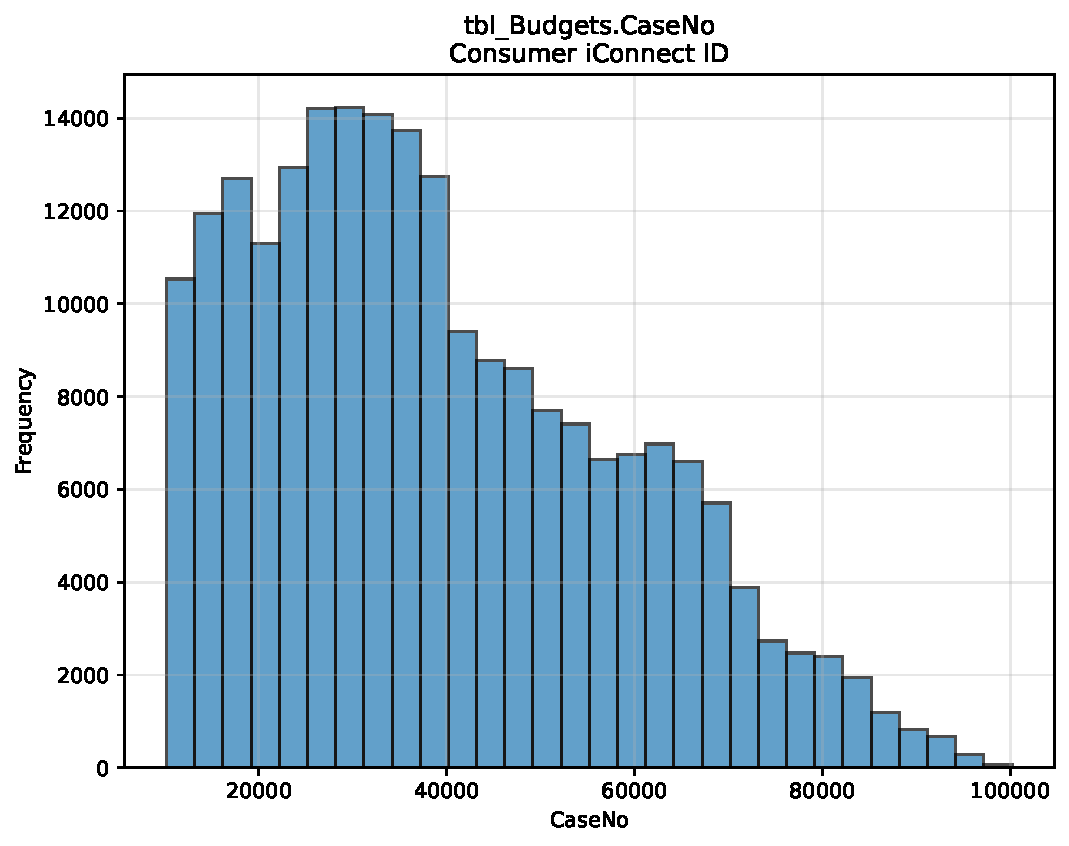
\includegraphics[width=\textwidth]{figures/dbo_tbl_Budgets_CaseNo.pdf}
\caption{Distribution of CaseNo in tbl\_Budgets}
\end{figure}\newpage

\subsection{tbl\_Budgets.BudgetID}
\textit{Budget ID}

\begin{figure}[htbp]
\centering
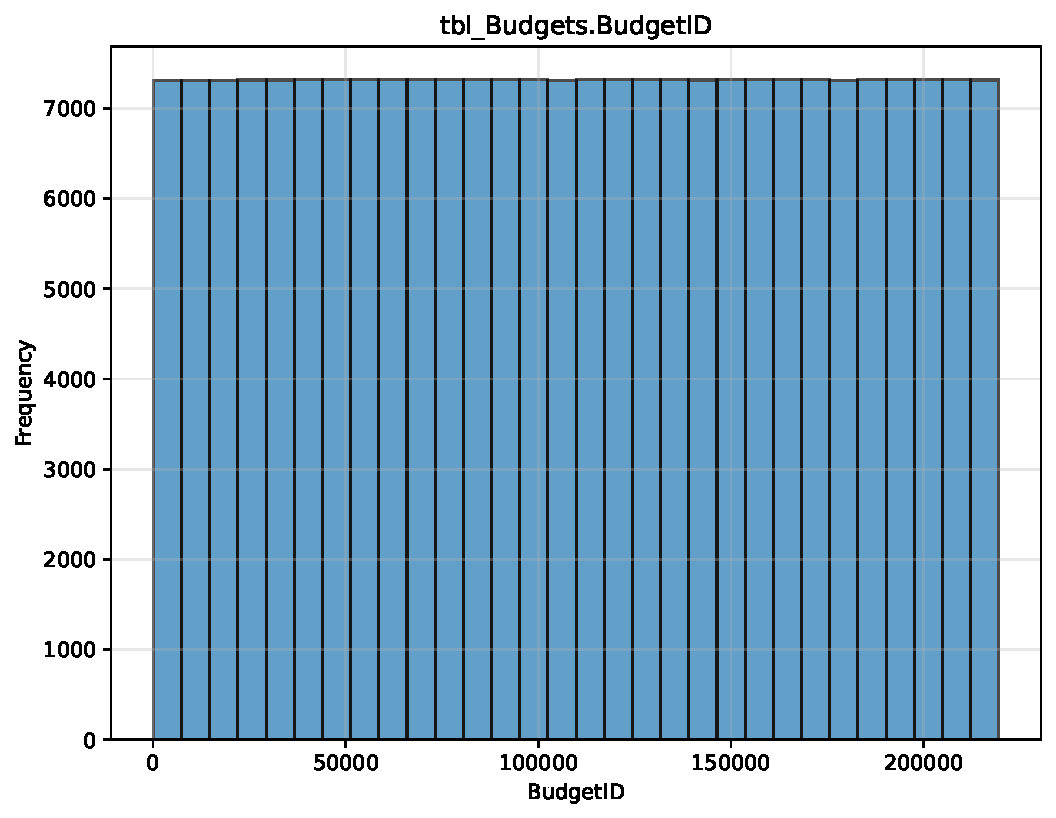
\includegraphics[width=\textwidth]{figures/dbo_tbl_Budgets_BudgetID.pdf}
\caption{Distribution of BudgetID in tbl\_Budgets}
\end{figure}\newpage

\subsection{tbl\_Budgets.ApprovedBy}
\textit{Approved By APD Staff Name}

\begin{figure}[htbp]
\centering
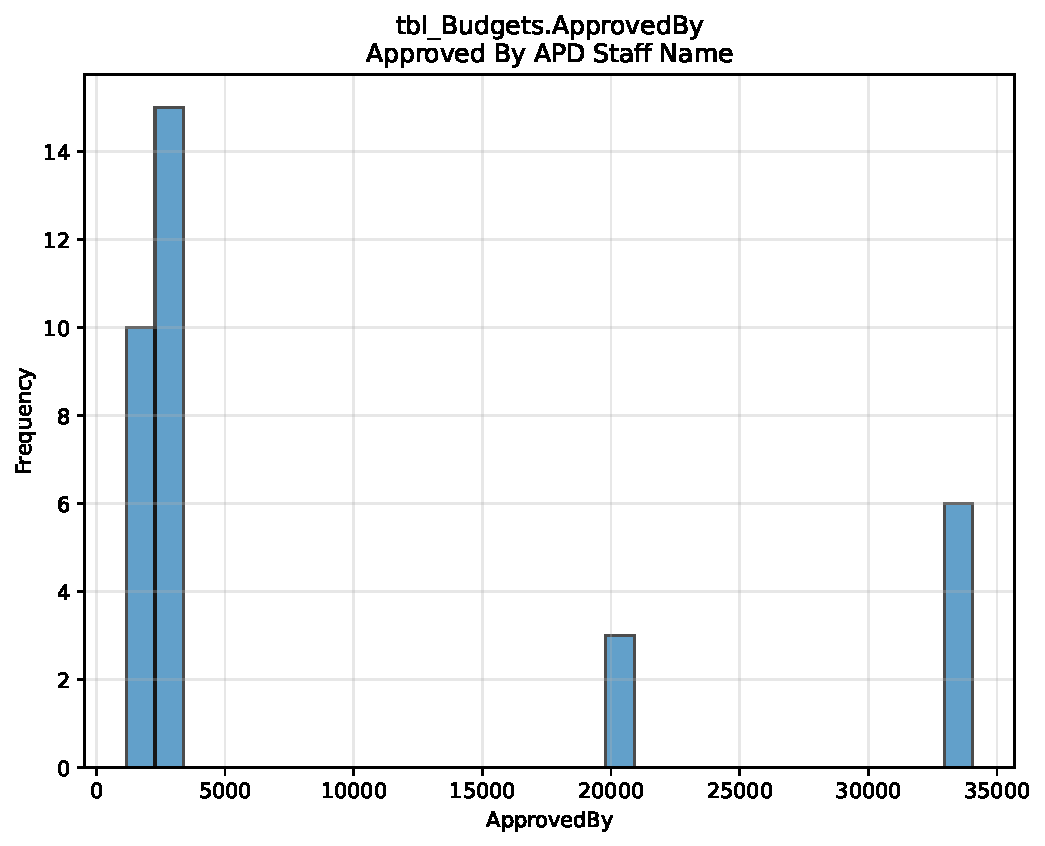
\includegraphics[width=\textwidth]{figures/dbo_tbl_Budgets_ApprovedBy.pdf}
\caption{Distribution of ApprovedBy in tbl\_Budgets}
\end{figure}\newpage

\subsection{tbl\_Budgets.BudgetAmount}
\textit{Budget Amount}

\begin{figure}[htbp]
\centering
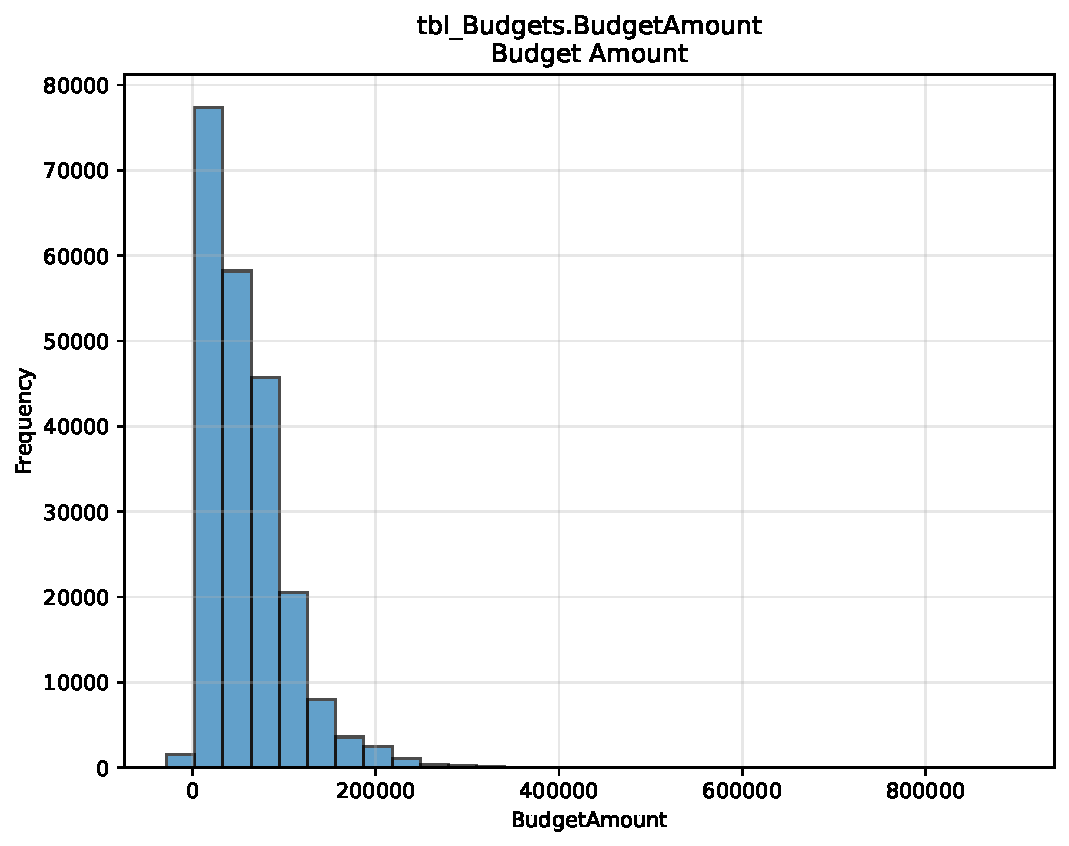
\includegraphics[width=\textwidth]{figures/dbo_tbl_Budgets_BudgetAmount.pdf}
\caption{Distribution of BudgetAmount in tbl\_Budgets}
\end{figure}\newpage

\subsection{tbl\_Budgets.AnnualizedAmount}
\textit{Annualized Budget Amount}

\begin{figure}[htbp]
\centering
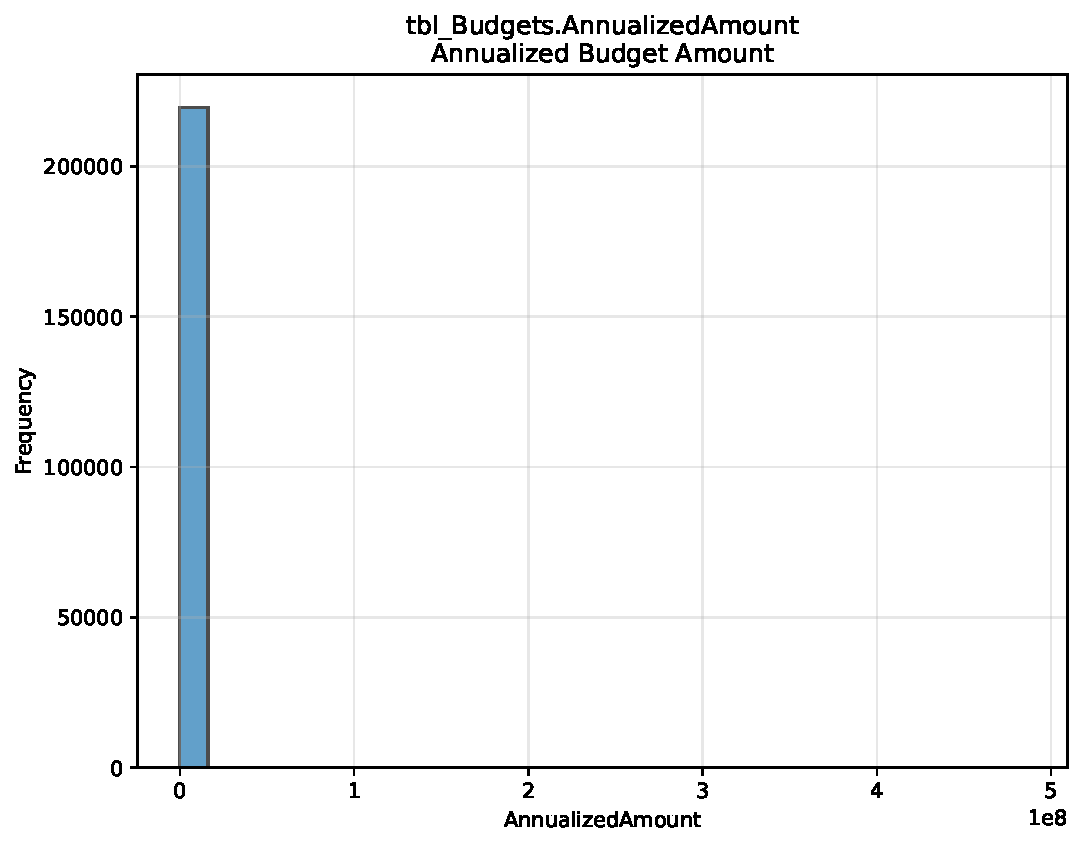
\includegraphics[width=\textwidth]{figures/dbo_tbl_Budgets_AnnualizedAmount.pdf}
\caption{Distribution of AnnualizedAmount in tbl\_Budgets}
\end{figure}\newpage

\subsection{tbl\_Budgets.AmountEncumbered}
\textit{Amount Encumbered}

\begin{figure}[htbp]
\centering
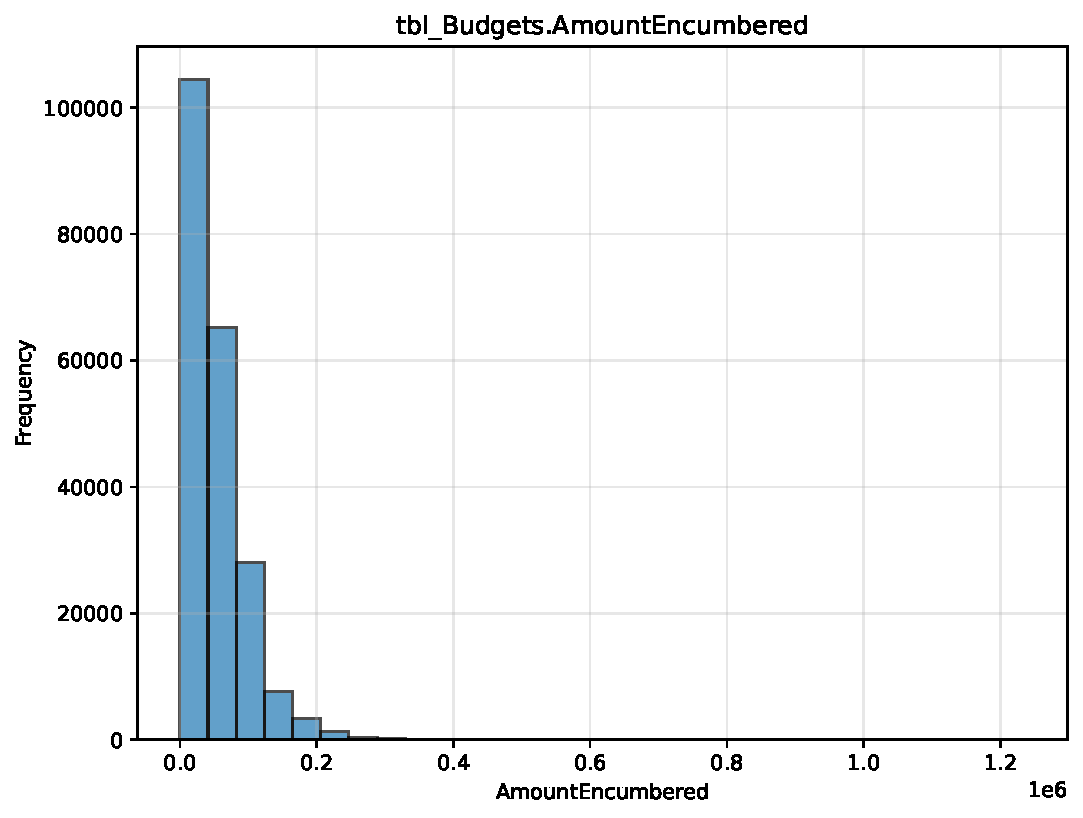
\includegraphics[width=\textwidth]{figures/dbo_tbl_Budgets_AmountEncumbered.pdf}
\caption{Distribution of AmountEncumbered in tbl\_Budgets}
\end{figure}\newpage

\subsection{tbl\_Budgets.AmountUnauthorized}
\textit{Amount Unauthorized}

\begin{figure}[htbp]
\centering
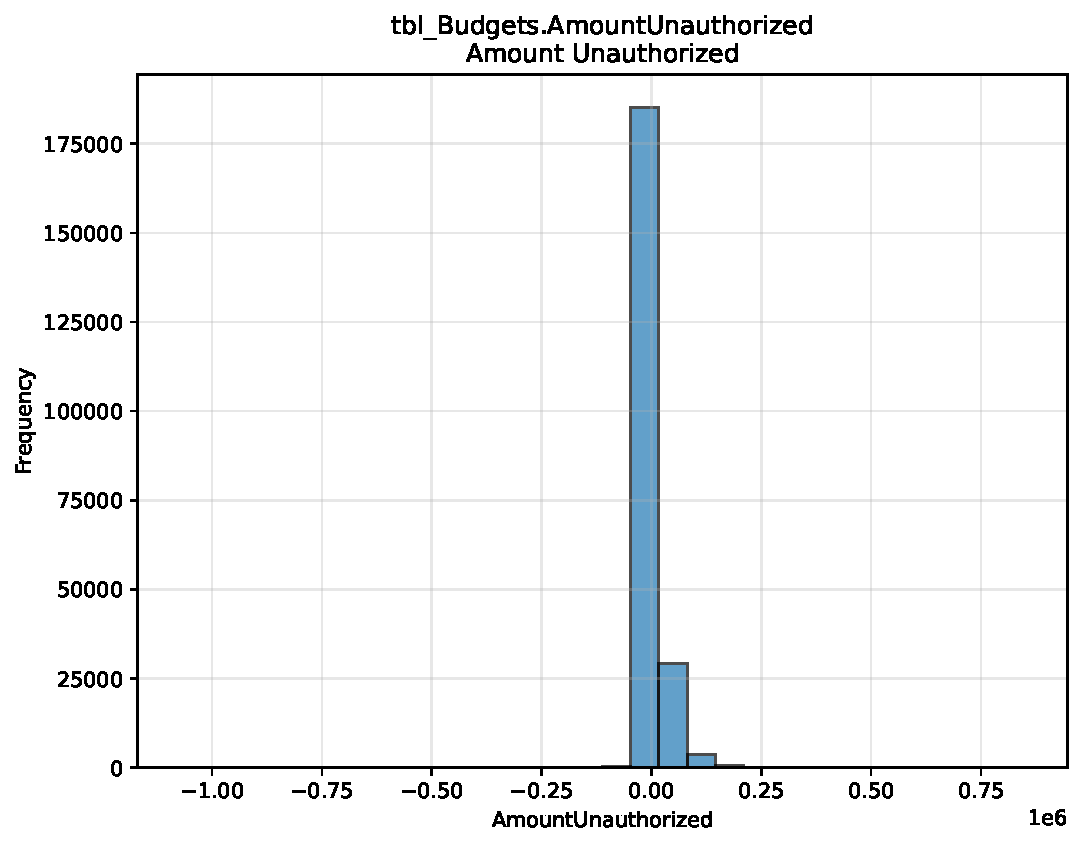
\includegraphics[width=\textwidth]{figures/dbo_tbl_Budgets_AmountUnauthorized.pdf}
\caption{Distribution of AmountUnauthorized in tbl\_Budgets}
\end{figure}\newpage

\subsection{tbl\_Budgets.PrioriBudgetAmount}
\textit{Priori Budget Amount}

\begin{figure}[htbp]
\centering
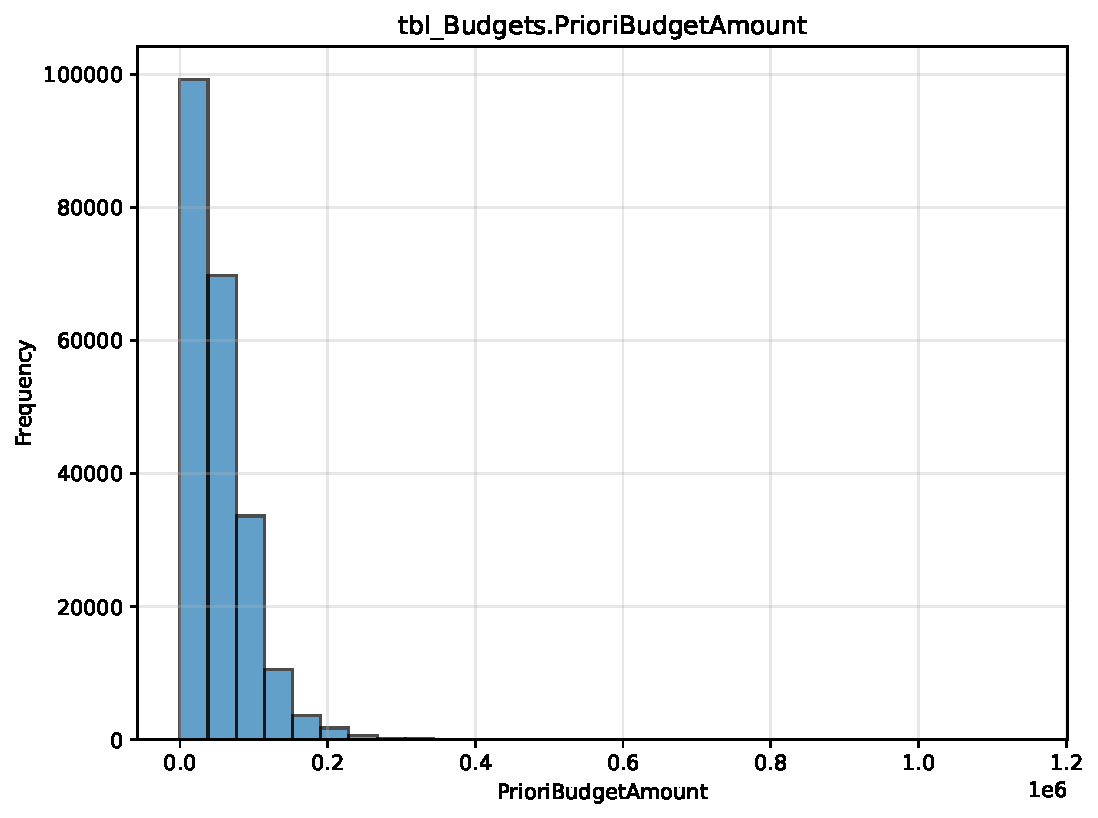
\includegraphics[width=\textwidth]{figures/dbo_tbl_Budgets_PrioriBudgetAmount.pdf}
\caption{Distribution of PrioriBudgetAmount in tbl\_Budgets}
\end{figure}\newpage

\subsection{tbl\_Claims\_MMIS.CaseNo}
\textit{Consumer iConnect ID}

\begin{figure}[htbp]
\centering
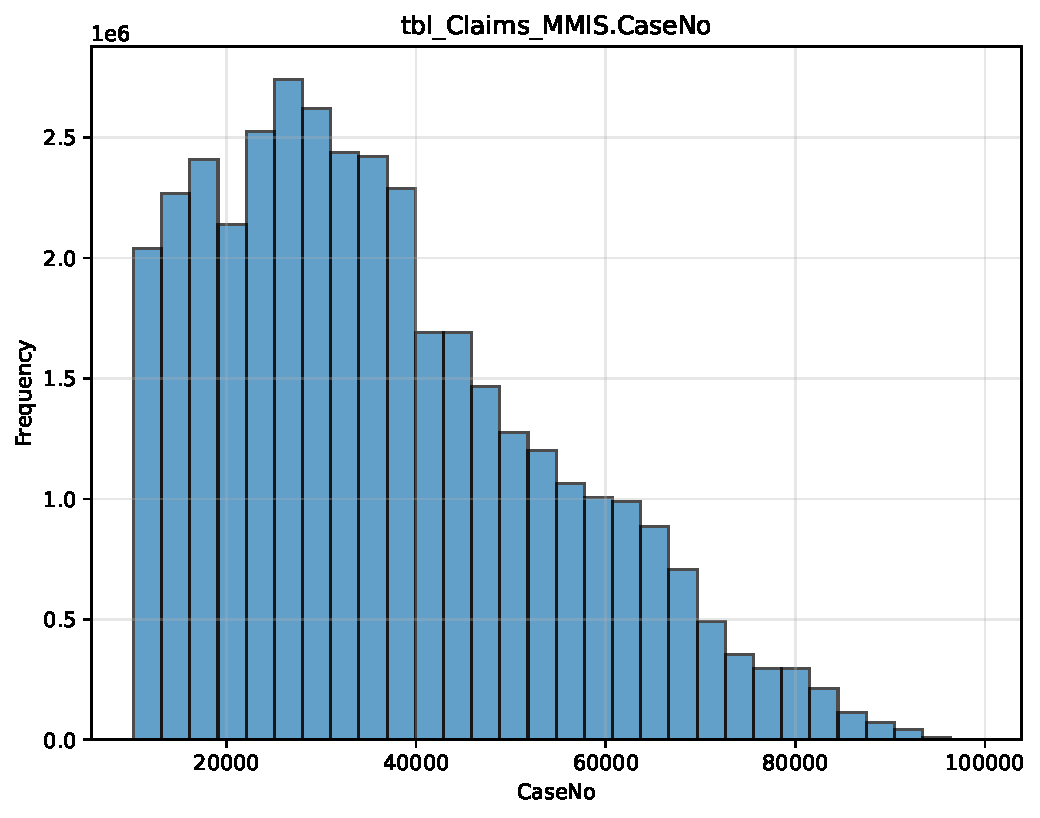
\includegraphics[width=\textwidth]{figures/dbo_tbl_Claims_MMIS_CaseNo.pdf}
\caption{Distribution of CaseNo in tbl\_Claims\_MMIS}
\end{figure}\newpage

\subsection{tbl\_Claims\_MMIS.Units}
\textit{Units}

\begin{figure}[htbp]
\centering
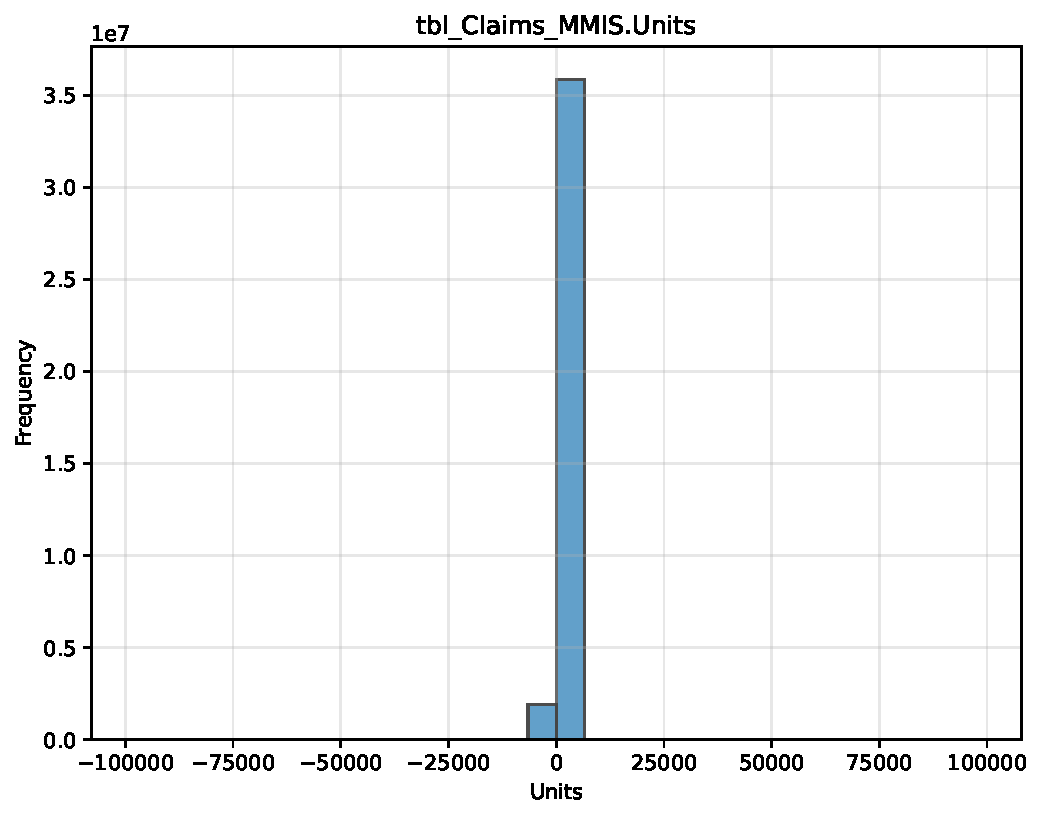
\includegraphics[width=\textwidth]{figures/dbo_tbl_Claims_MMIS_Units.pdf}
\caption{Distribution of Units in tbl\_Claims\_MMIS}
\end{figure}\newpage

\subsection{tbl\_Claims\_MMIS.BilledAmt}
\textit{Billed Amount}

\begin{figure}[htbp]
\centering
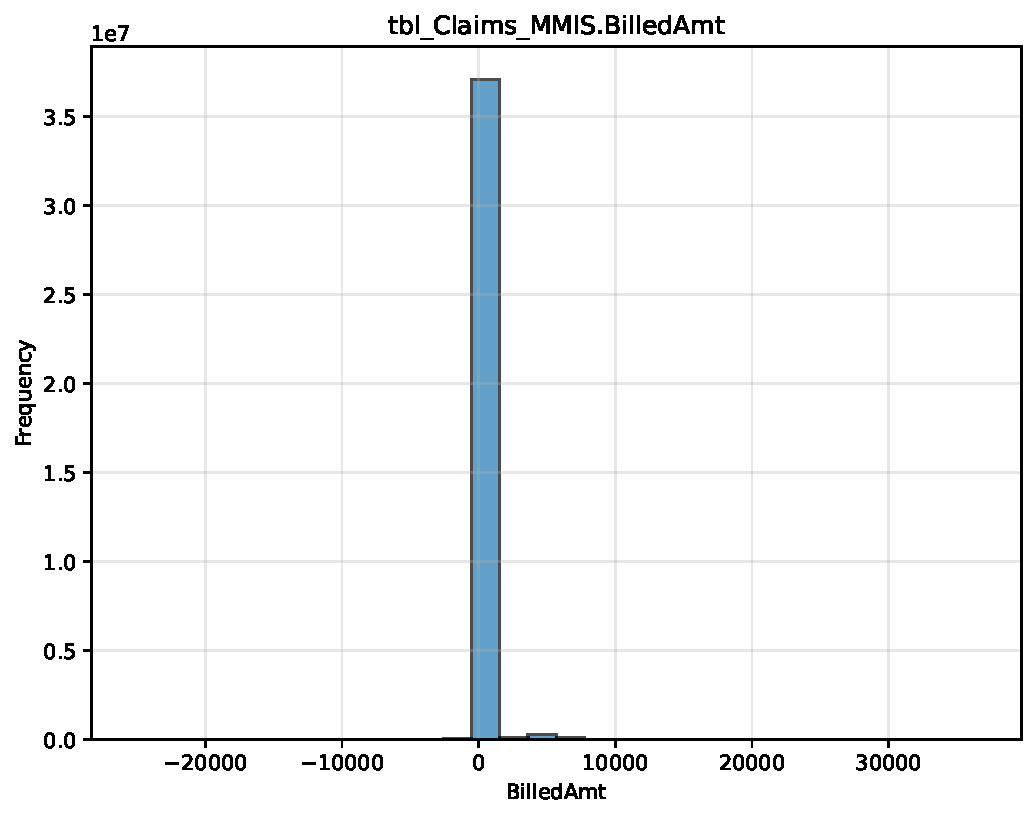
\includegraphics[width=\textwidth]{figures/dbo_tbl_Claims_MMIS_BilledAmt.pdf}
\caption{Distribution of BilledAmt in tbl\_Claims\_MMIS}
\end{figure}\newpage

\subsection{tbl\_Claims\_MMIS.PaidAmt}
\textit{Paid Amount}

\begin{figure}[htbp]
\centering
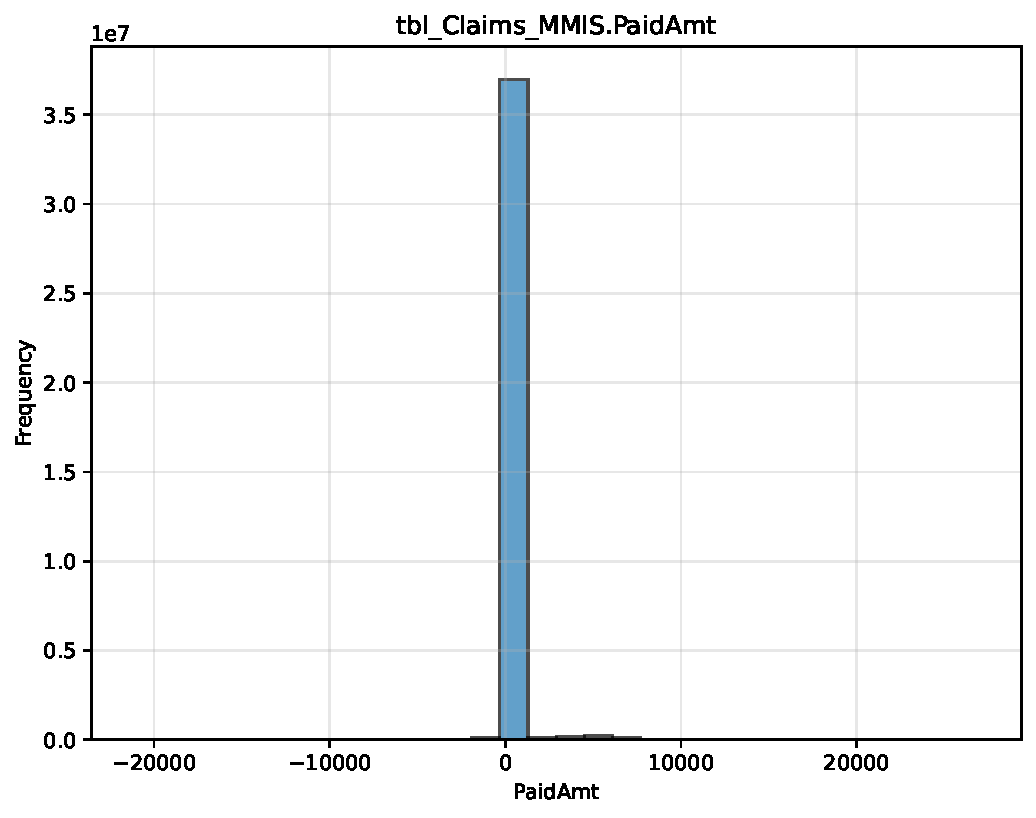
\includegraphics[width=\textwidth]{figures/dbo_tbl_Claims_MMIS_PaidAmt.pdf}
\caption{Distribution of PaidAmt in tbl\_Claims\_MMIS}
\end{figure}\newpage

\subsection{tbl\_Claims\_MMIS.Id}
\textit{Claim ID}

\begin{figure}[htbp]
\centering
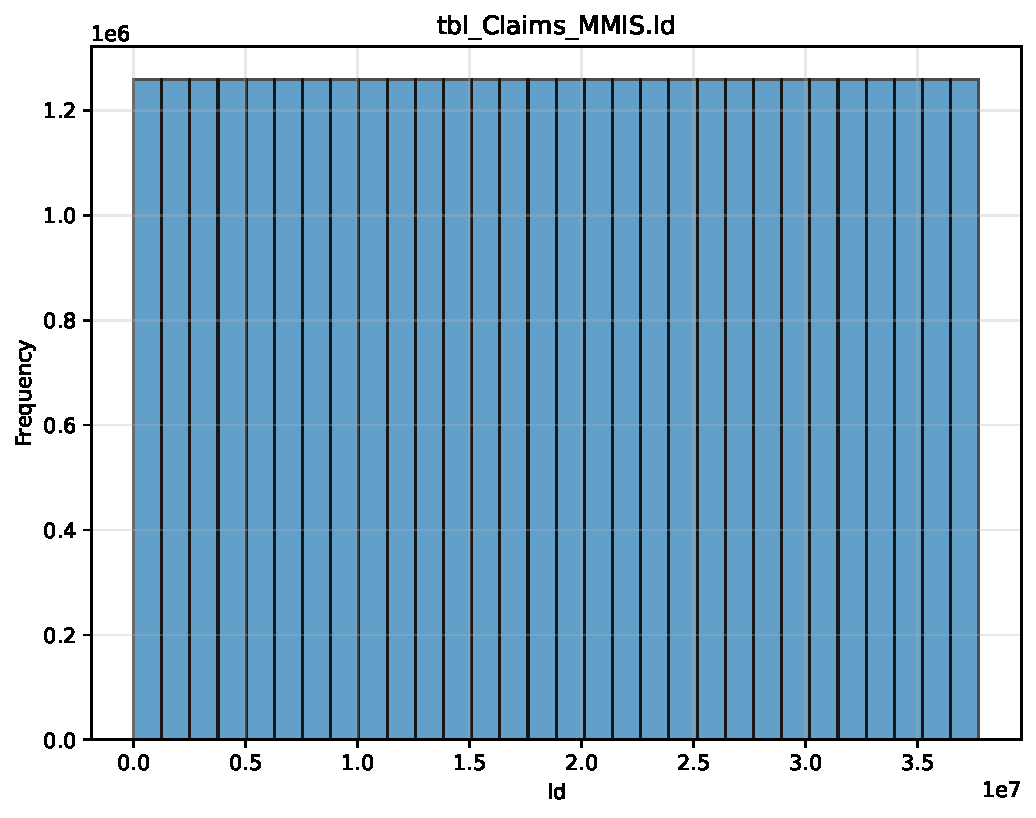
\includegraphics[width=\textwidth]{figures/dbo_tbl_Claims_MMIS_Id.pdf}
\caption{Distribution of Id in tbl\_Claims\_MMIS}
\end{figure}\newpage

\subsection{tbl\_ConsumerContacts.CONTACTID}
\textit{Contact ID}

\begin{figure}[htbp]
\centering
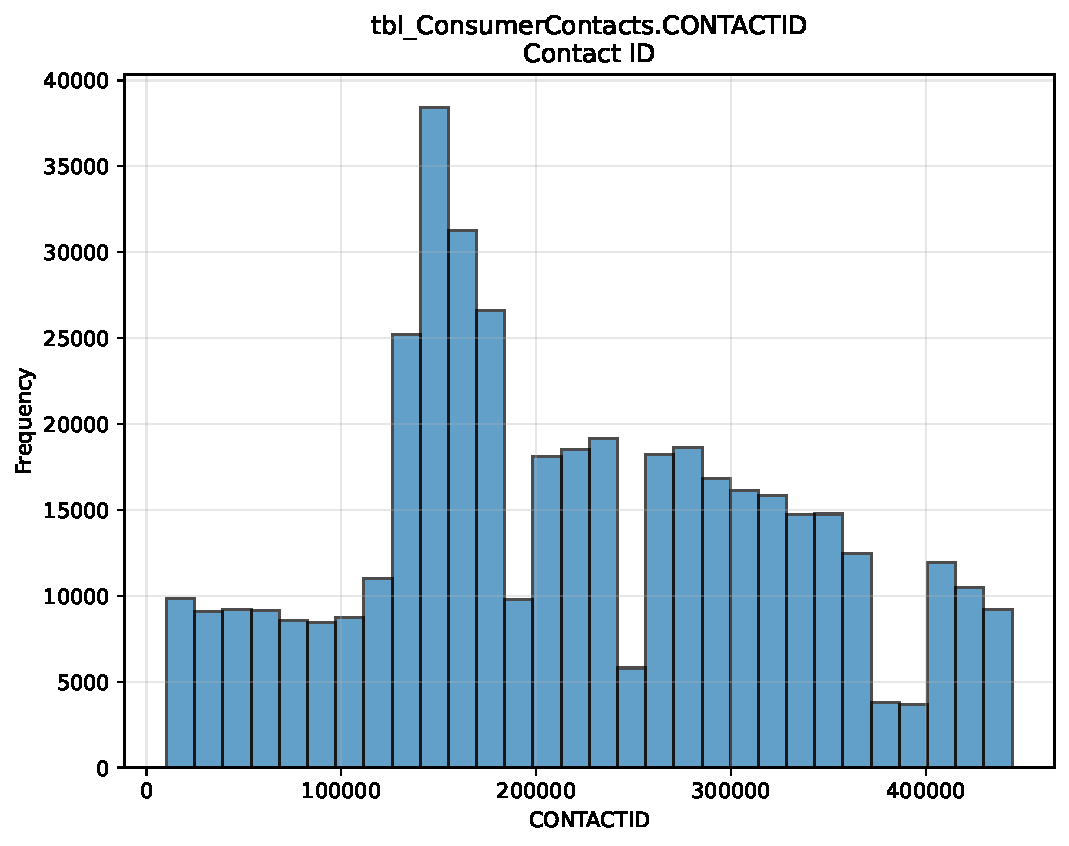
\includegraphics[width=\textwidth]{figures/dbo_tbl_ConsumerContacts_CONTACTID.pdf}
\caption{Distribution of CONTACTID in tbl\_ConsumerContacts}
\end{figure}\newpage

\subsection{tbl\_ConsumerContacts.CASENO}
\textit{Consumer iConnect ID}

\begin{figure}[htbp]
\centering
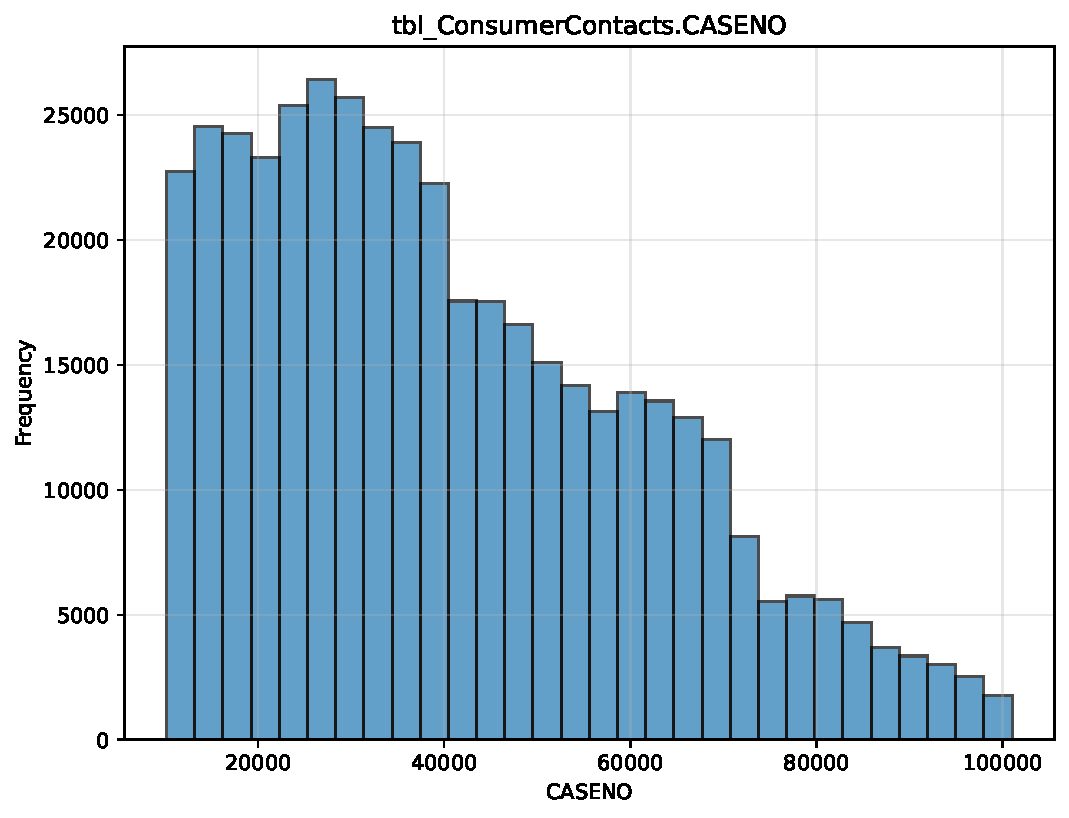
\includegraphics[width=\textwidth]{figures/dbo_tbl_ConsumerContacts_CASENO.pdf}
\caption{Distribution of CASENO in tbl\_ConsumerContacts}
\end{figure}\newpage

\subsection{tbl\_ConsumerContacts.Active}
\textit{Active}

\begin{figure}[htbp]
\centering
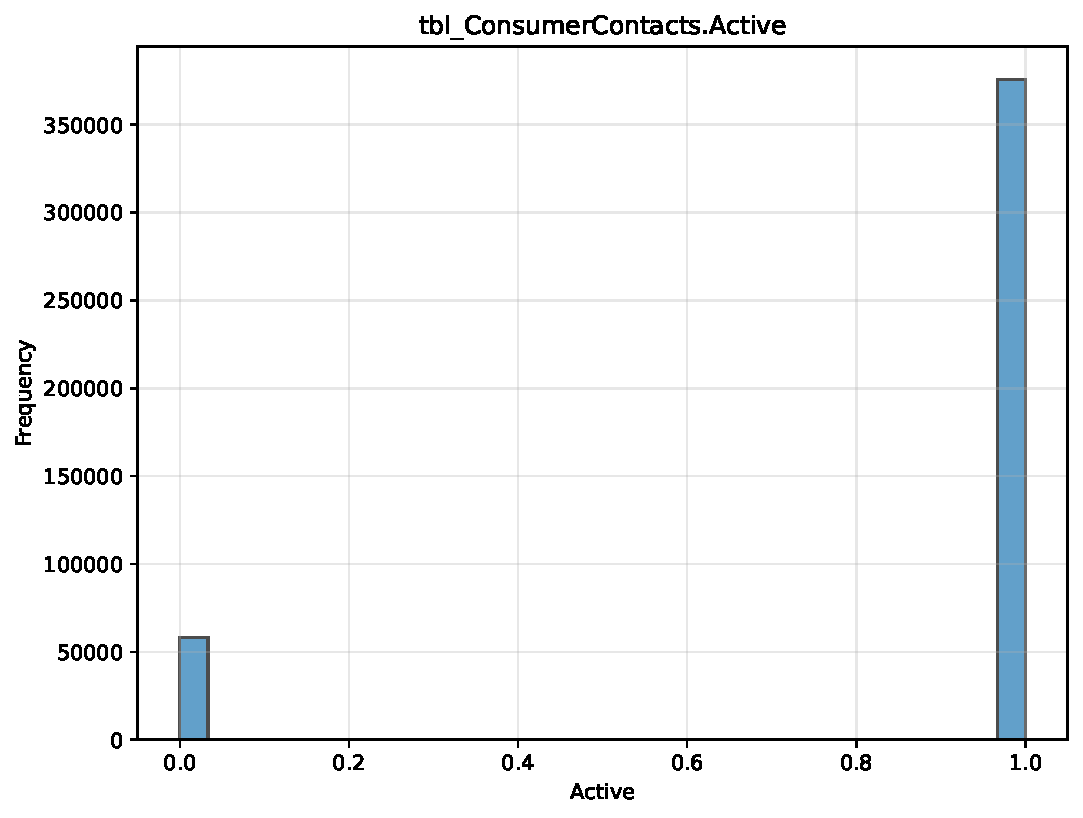
\includegraphics[width=\textwidth]{figures/dbo_tbl_ConsumerContacts_Active.pdf}
\caption{Distribution of Active in tbl\_ConsumerContacts}
\end{figure}\newpage

\subsection{tbl\_ConsumerContacts.RECID}
\textit{Record ID}

\begin{figure}[htbp]
\centering
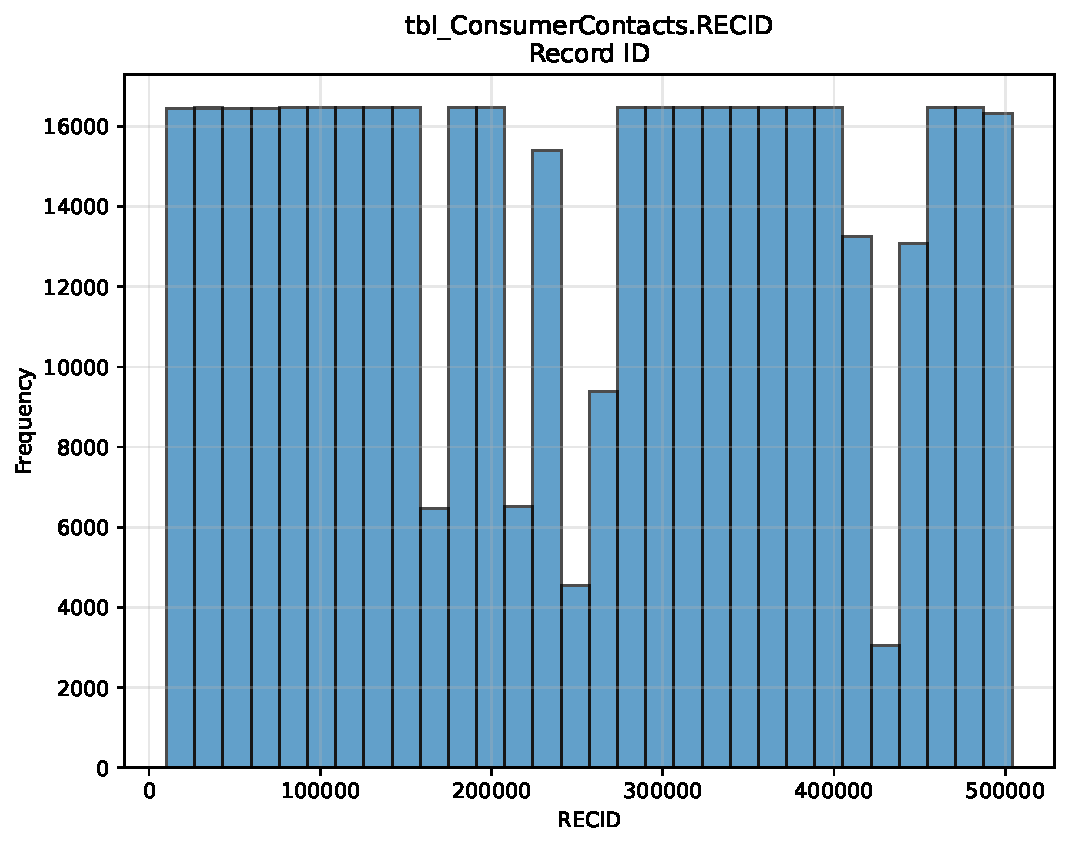
\includegraphics[width=\textwidth]{figures/dbo_tbl_ConsumerContacts_RECID.pdf}
\caption{Distribution of RECID in tbl\_ConsumerContacts}
\end{figure}\newpage

\subsection{tbl\_Consumers.CASENO}
\textit{Consumer iConnect ID}

\begin{figure}[htbp]
\centering
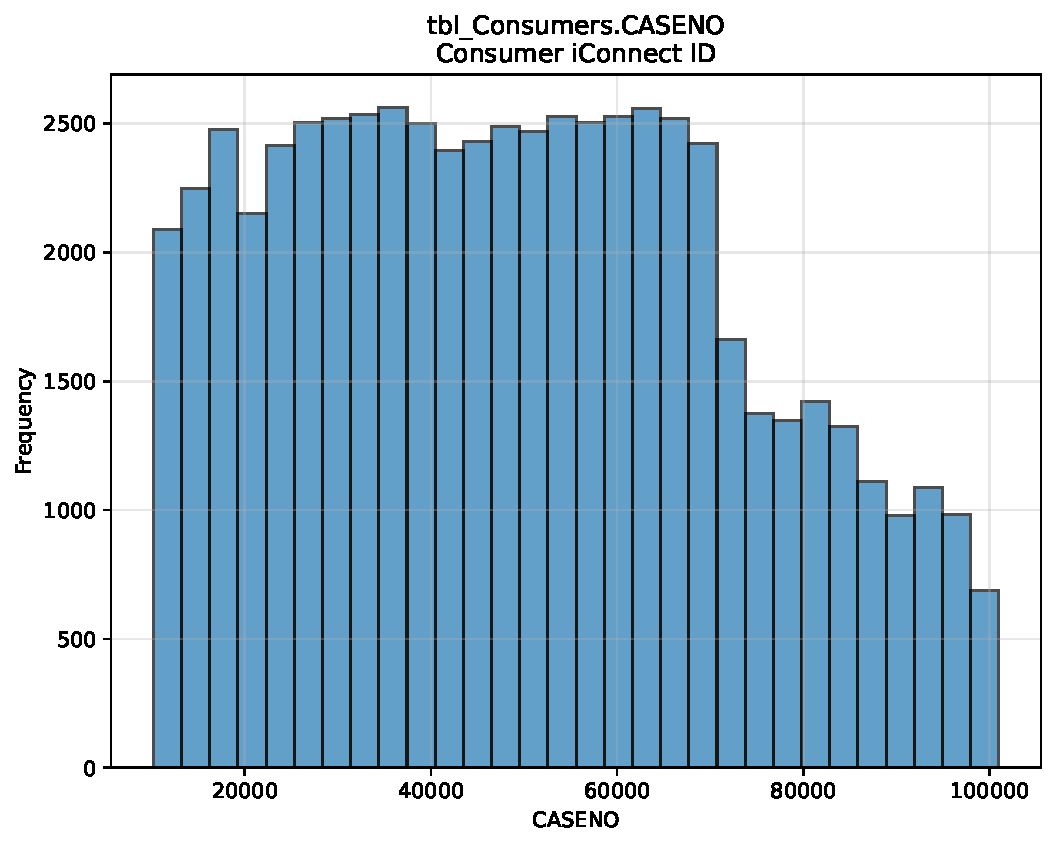
\includegraphics[width=\textwidth]{figures/dbo_tbl_Consumers_CASENO.pdf}
\caption{Distribution of CASENO in tbl\_Consumers}
\end{figure}\newpage

\subsection{tbl\_Consumers.CBCFlag}
\textit{CBC Flag- Identifies if the Consumer has enrolled in CBC Program}

\begin{figure}[htbp]
\centering
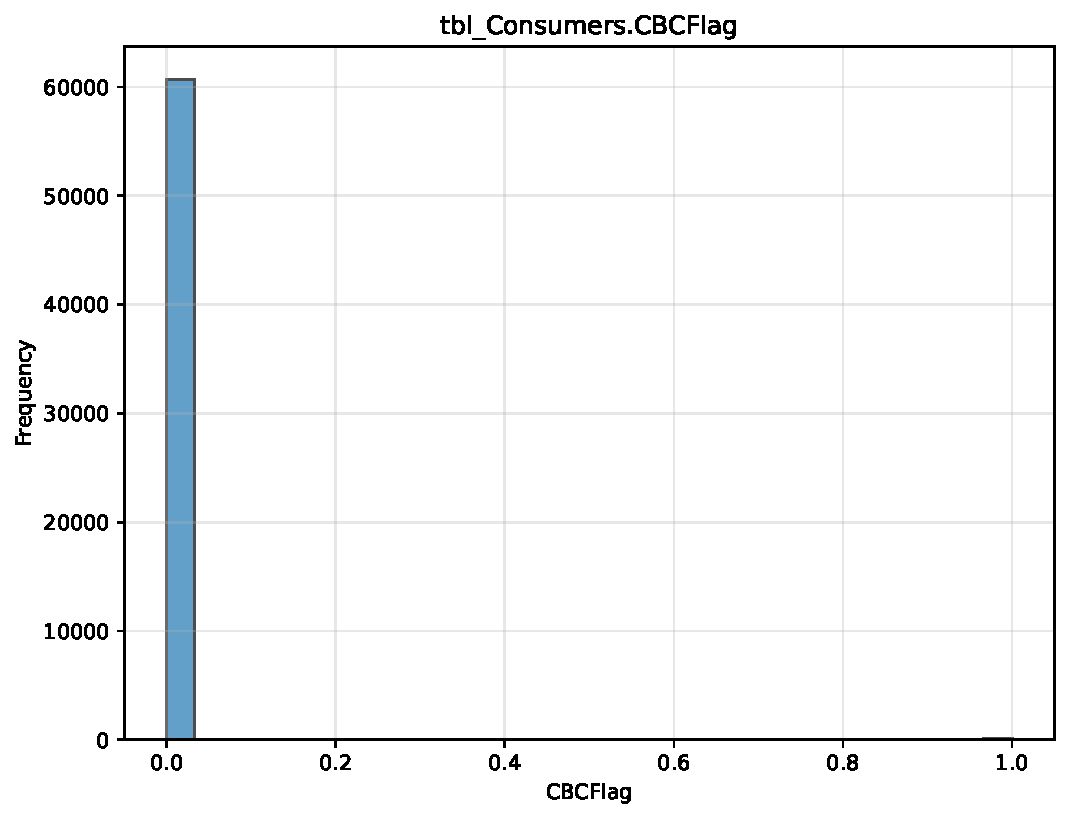
\includegraphics[width=\textwidth]{figures/dbo_tbl_Consumers_CBCFlag.pdf}
\caption{Distribution of CBCFlag in tbl\_Consumers}
\end{figure}\newpage

\subsection{tbl\_Consumers.ANNUALINCOME}
\textit{ANNUAL INCOME}

\begin{figure}[htbp]
\centering
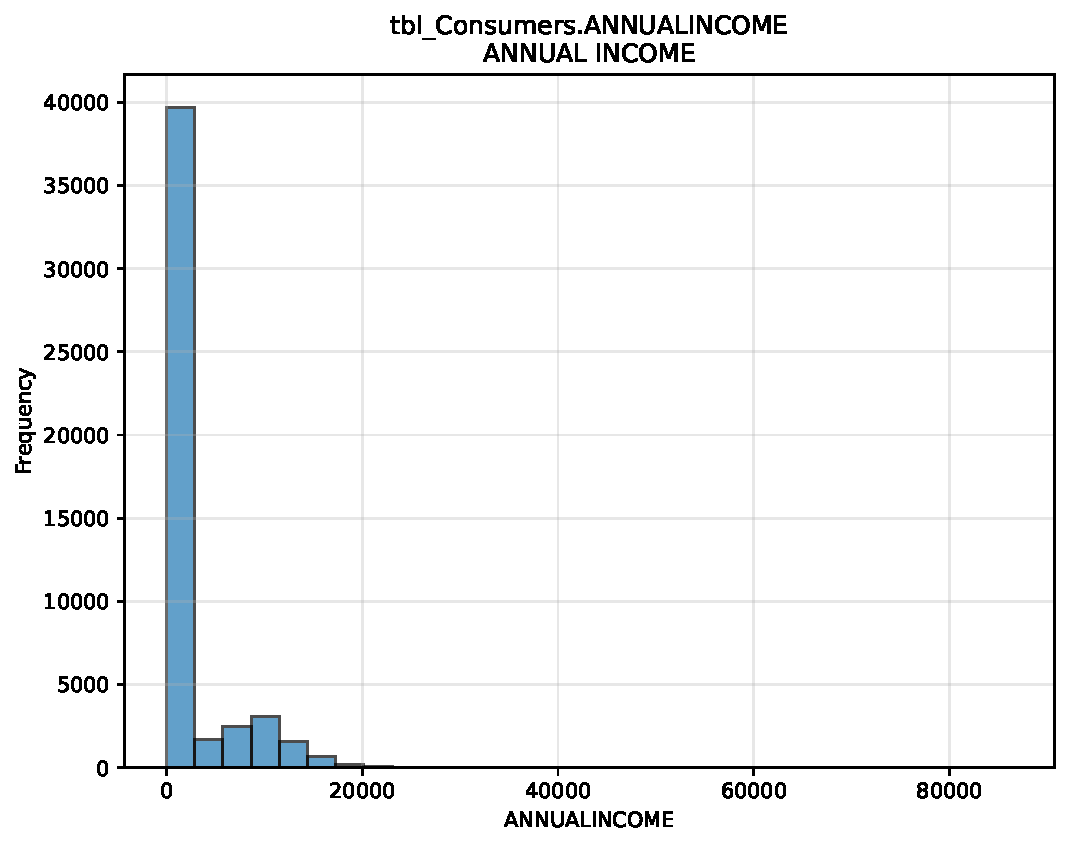
\includegraphics[width=\textwidth]{figures/dbo_tbl_Consumers_ANNUALINCOME.pdf}
\caption{Distribution of ANNUALINCOME in tbl\_Consumers}
\end{figure}\newpage

\subsection{tbl\_Consumers.OPENID}
\textit{Open ID}

\begin{figure}[htbp]
\centering
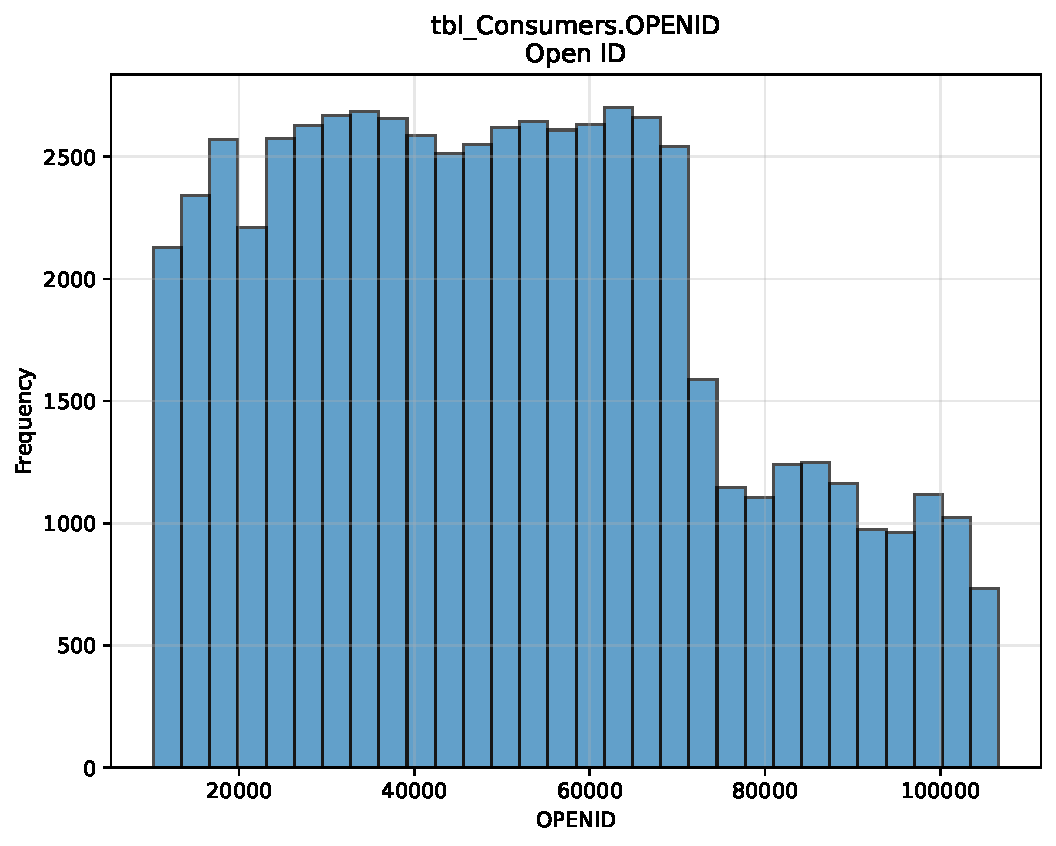
\includegraphics[width=\textwidth]{figures/dbo_tbl_Consumers_OPENID.pdf}
\caption{Distribution of OPENID in tbl\_Consumers}
\end{figure}\newpage

\subsection{tbl\_Consumers.PRIMARYWORKERID}
\textit{Primary Worker ID}

\begin{figure}[htbp]
\centering
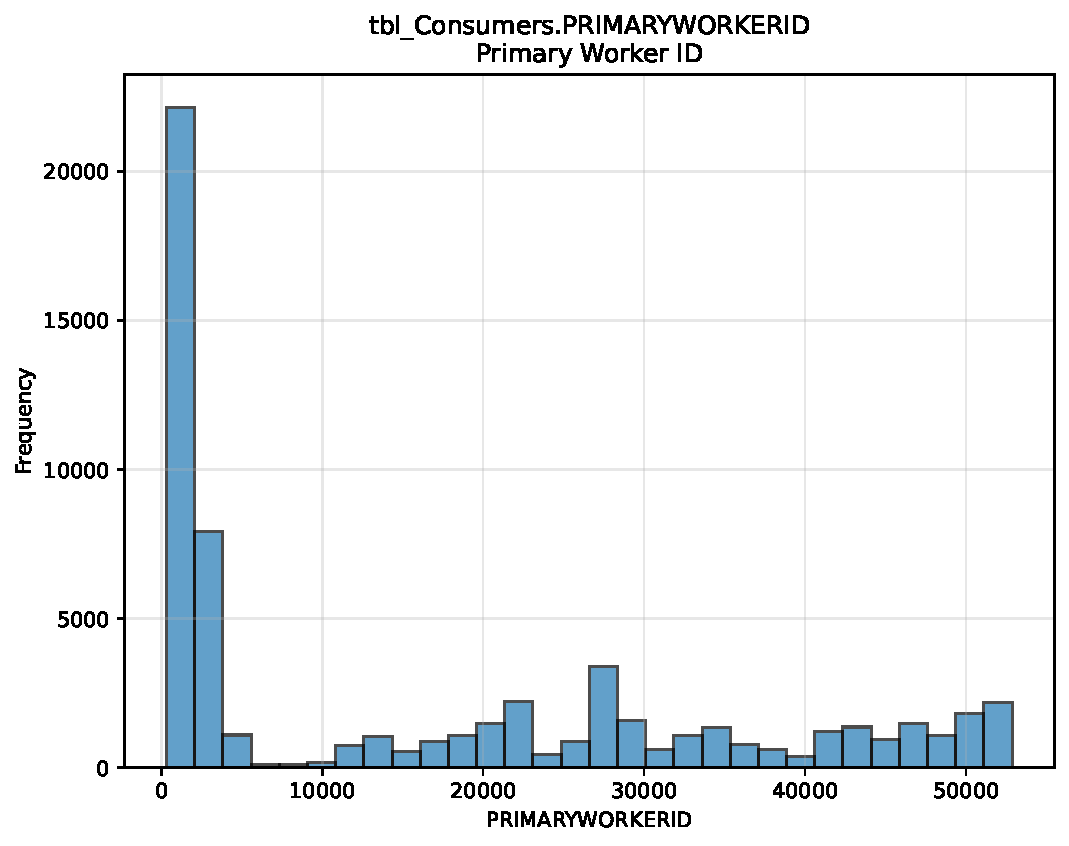
\includegraphics[width=\textwidth]{figures/dbo_tbl_Consumers_PRIMARYWORKERID.pdf}
\caption{Distribution of PRIMARYWORKERID in tbl\_Consumers}
\end{figure}\newpage

\subsection{tbl\_Consumers.SECONDWORKERID}
\textit{Secondary Worker ID}

\begin{figure}[htbp]
\centering
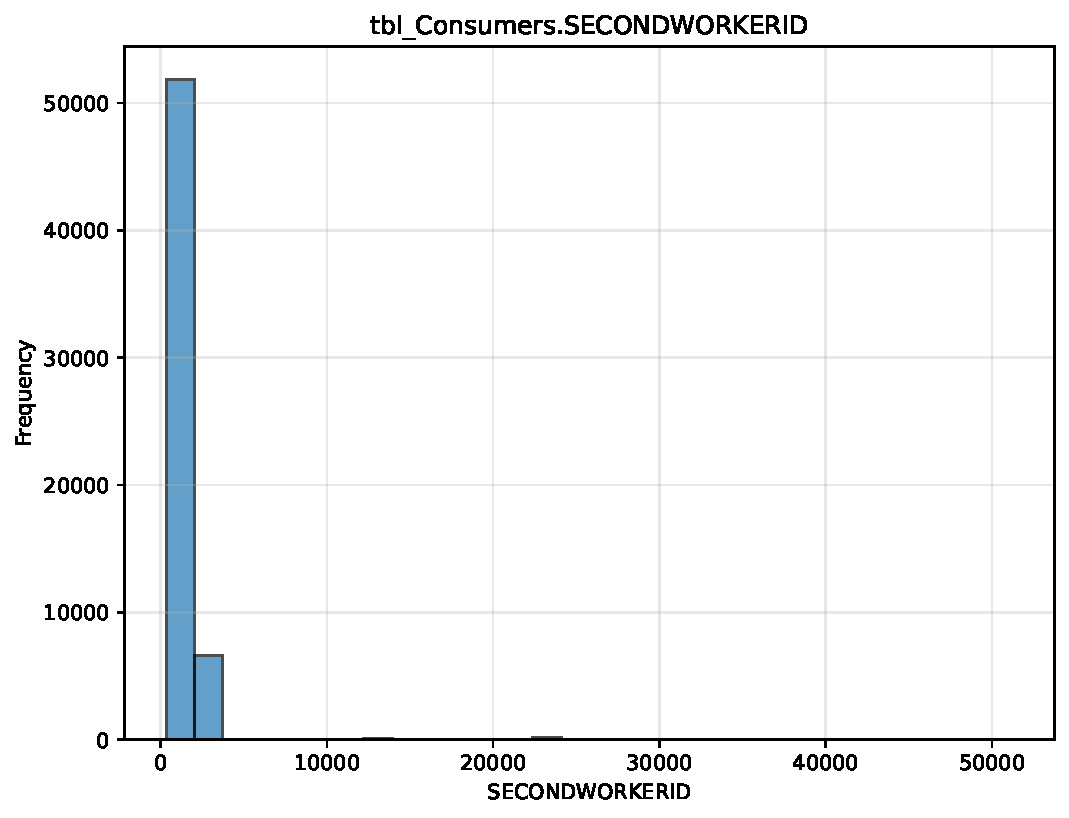
\includegraphics[width=\textwidth]{figures/dbo_tbl_Consumers_SECONDWORKERID.pdf}
\caption{Distribution of SECONDWORKERID in tbl\_Consumers}
\end{figure}\newpage

\subsection{tbl\_Consumers.CONTACTID}
\textit{Contact ID}

\begin{figure}[htbp]
\centering
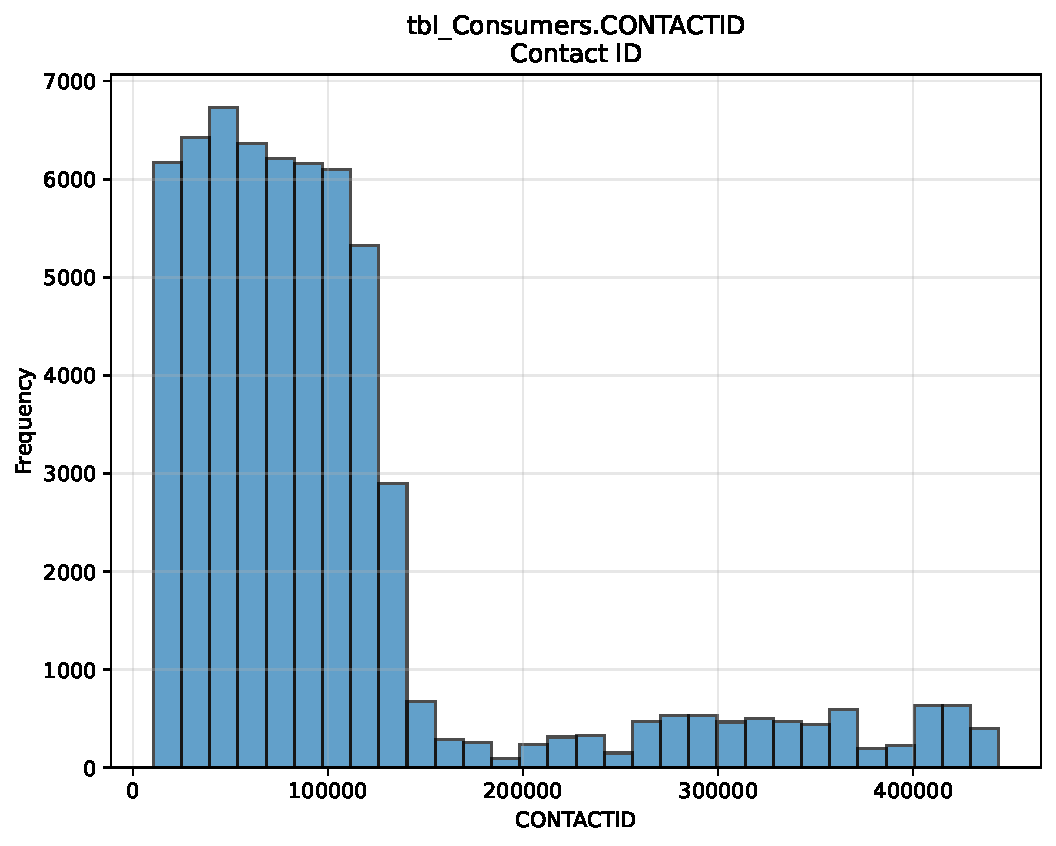
\includegraphics[width=\textwidth]{figures/dbo_tbl_Consumers_CONTACTID.pdf}
\caption{Distribution of CONTACTID in tbl\_Consumers}
\end{figure}\newpage

\subsection{tbl\_Consumers.Id}
\textit{Id}

\begin{figure}[htbp]
\centering
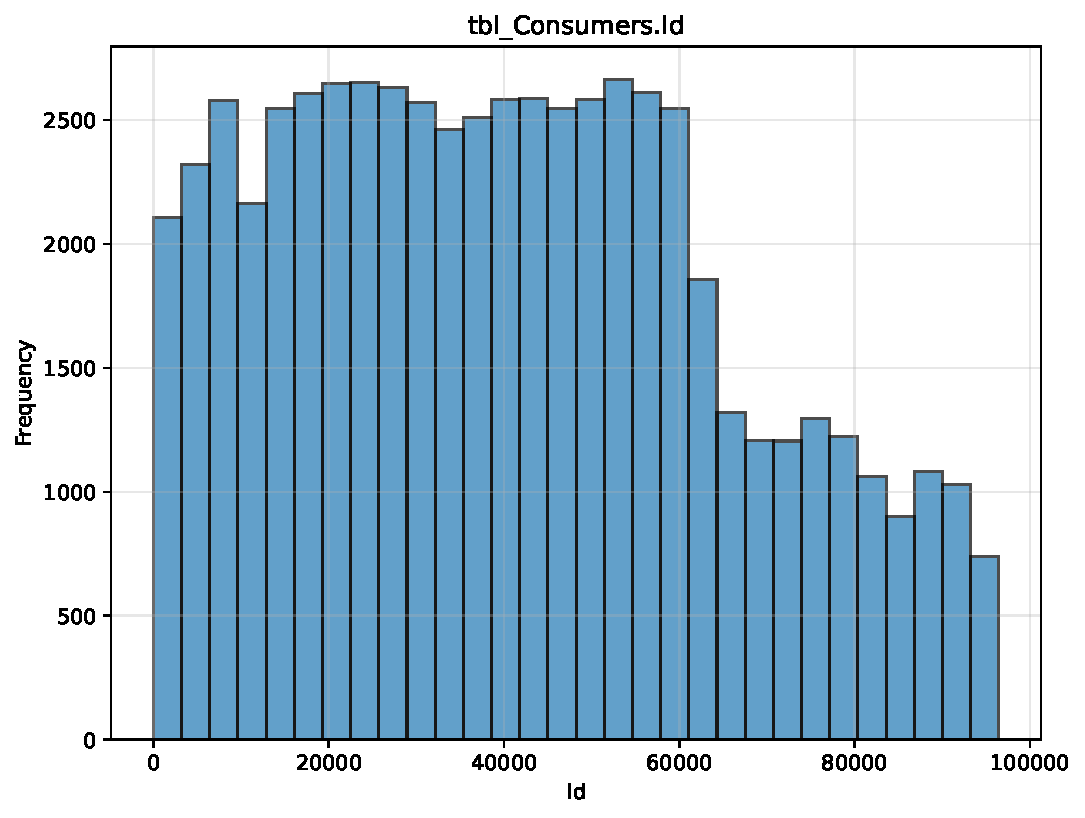
\includegraphics[width=\textwidth]{figures/dbo_tbl_Consumers_Id.pdf}
\caption{Distribution of Id in tbl\_Consumers}
\end{figure}\newpage

\subsection{tbl\_Diagnosis.CASENO}
\textit{Consumer iConnect ID}

\begin{figure}[htbp]
\centering
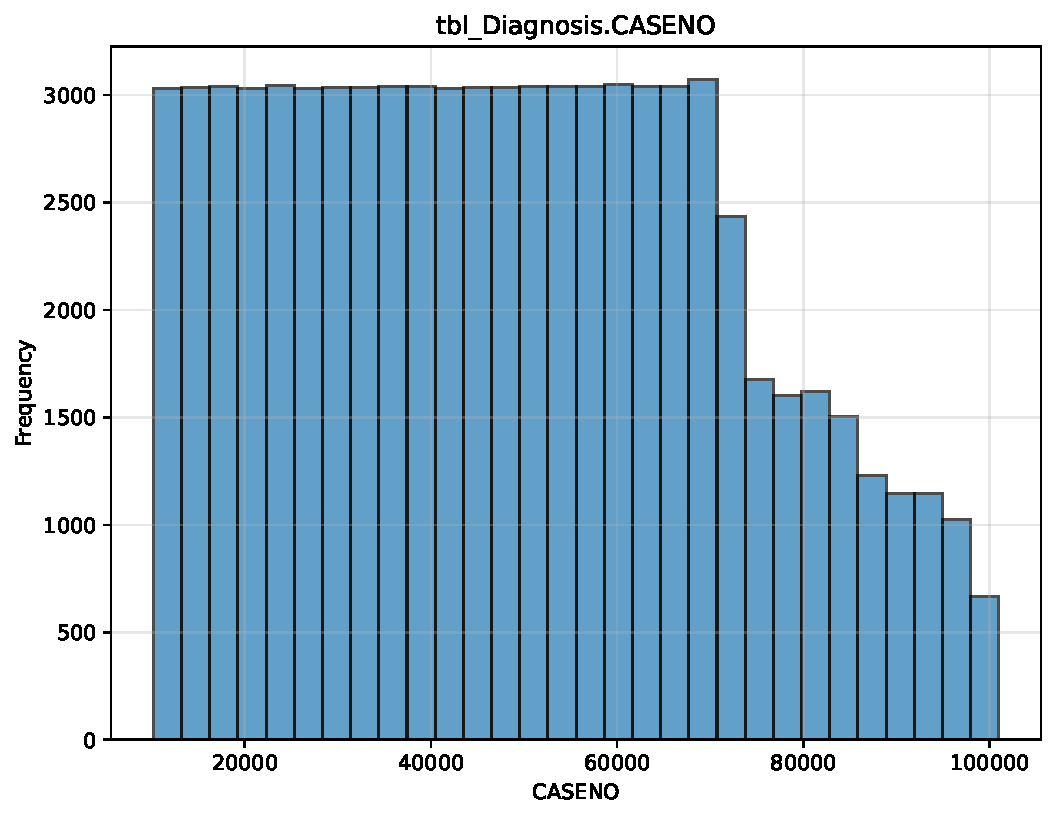
\includegraphics[width=\textwidth]{figures/dbo_tbl_Diagnosis_CASENO.pdf}
\caption{Distribution of CASENO in tbl\_Diagnosis}
\end{figure}\newpage

\subsection{tbl\_Diagnosis.DiagnosisID}
\textit{Diagnosis ID}

\begin{figure}[htbp]
\centering
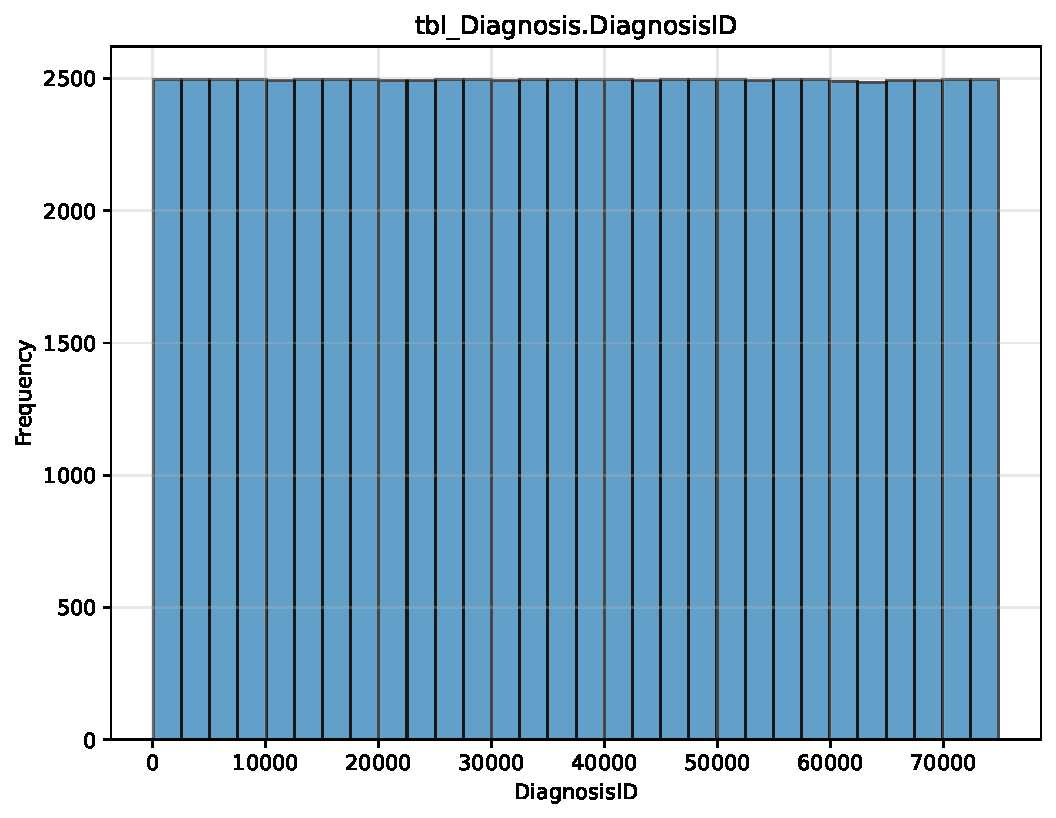
\includegraphics[width=\textwidth]{figures/dbo_tbl_Diagnosis_DiagnosisID.pdf}
\caption{Distribution of DiagnosisID in tbl\_Diagnosis}
\end{figure}\newpage

\subsection{tbl\_EZBudget.CASENO}
\textit{Consumer iConnect ID}

\begin{figure}[htbp]
\centering
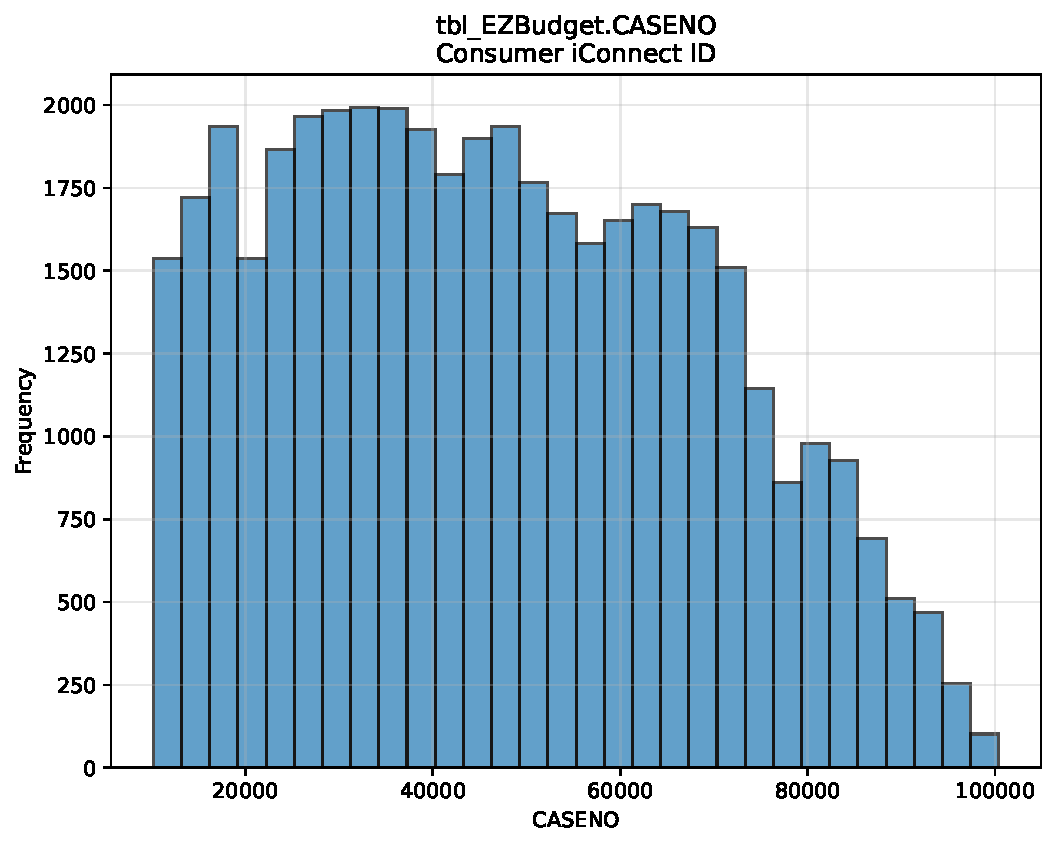
\includegraphics[width=\textwidth]{figures/dbo_tbl_EZBudget_CASENO.pdf}
\caption{Distribution of CASENO in tbl\_EZBudget}
\end{figure}\newpage

\subsection{tbl\_EZBudget.EZBudgetAssessId}
\textit{EZ iBudget Calculator Form ID}

\begin{figure}[htbp]
\centering
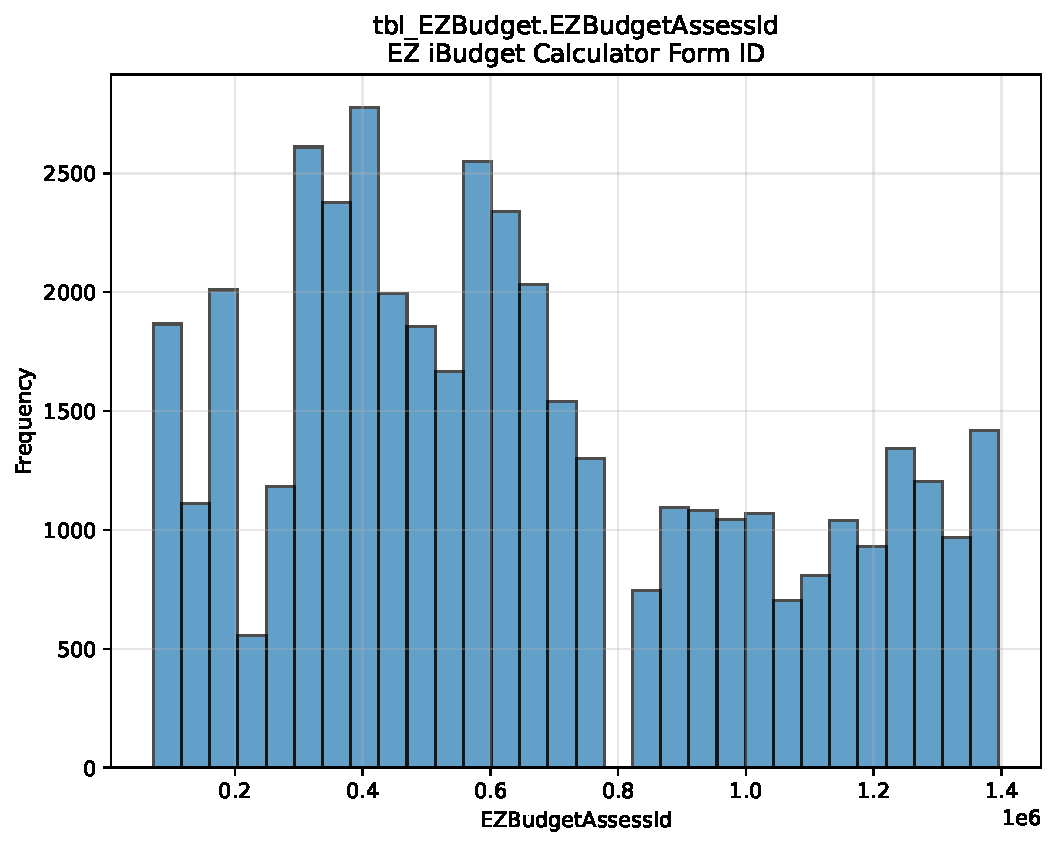
\includegraphics[width=\textwidth]{figures/dbo_tbl_EZBudget_EZBudgetAssessId.pdf}
\caption{Distribution of EZBudgetAssessId in tbl\_EZBudget}
\end{figure}\newpage

\subsection{tbl\_PlannedServices.CaseNo}
\textit{Consumer iConnect ID}

\begin{figure}[htbp]
\centering
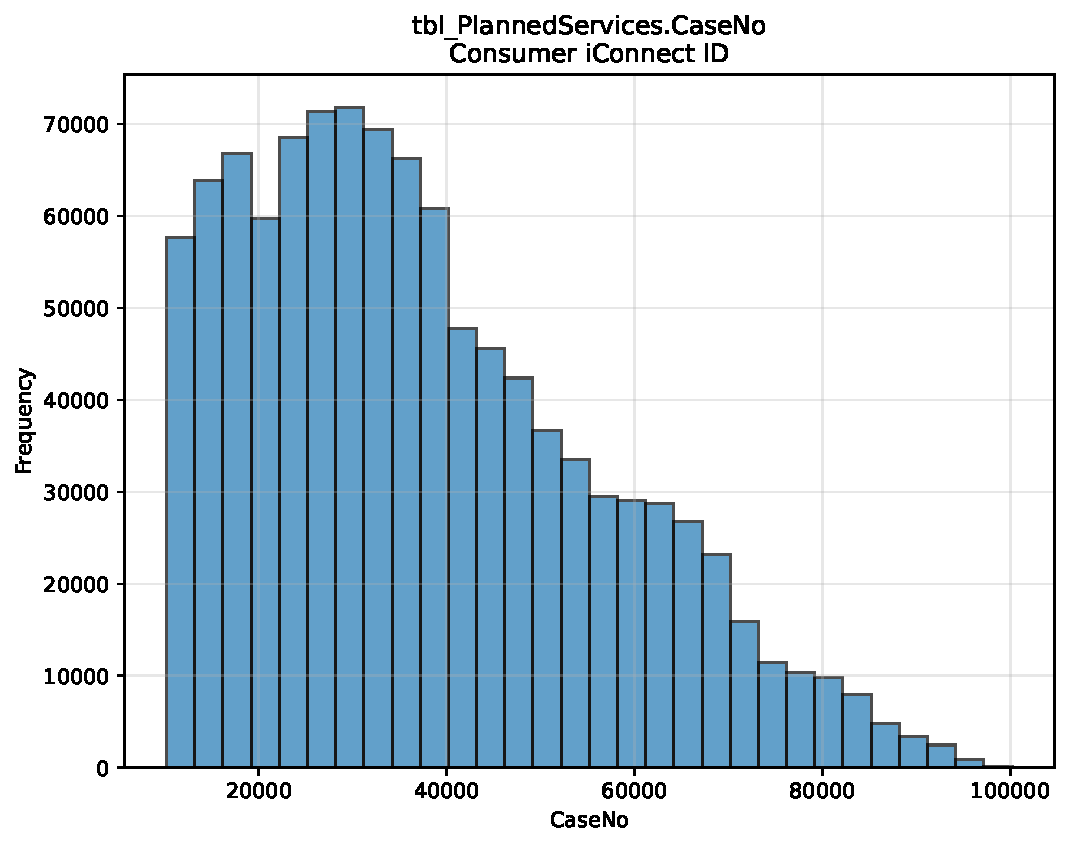
\includegraphics[width=\textwidth]{figures/dbo_tbl_PlannedServices_CaseNo.pdf}
\caption{Distribution of CaseNo in tbl\_PlannedServices}
\end{figure}\newpage

\subsection{tbl\_PlannedServices.FiscalYear}
\textit{FiscalYear}

\begin{figure}[htbp]
\centering
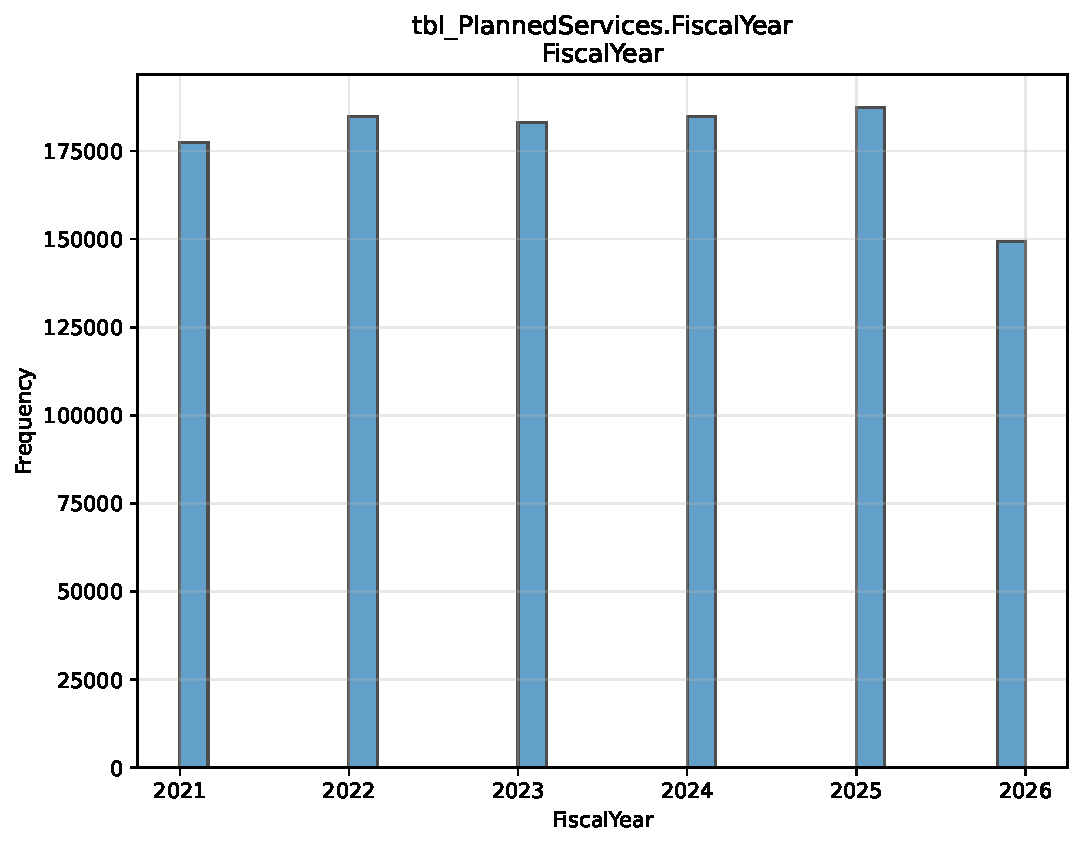
\includegraphics[width=\textwidth]{figures/dbo_tbl_PlannedServices_FiscalYear.pdf}
\caption{Distribution of FiscalYear in tbl\_PlannedServices}
\end{figure}\newpage

\subsection{tbl\_PlannedServices.UnitsPer}
\textit{UnitsPer}

\begin{figure}[htbp]
\centering
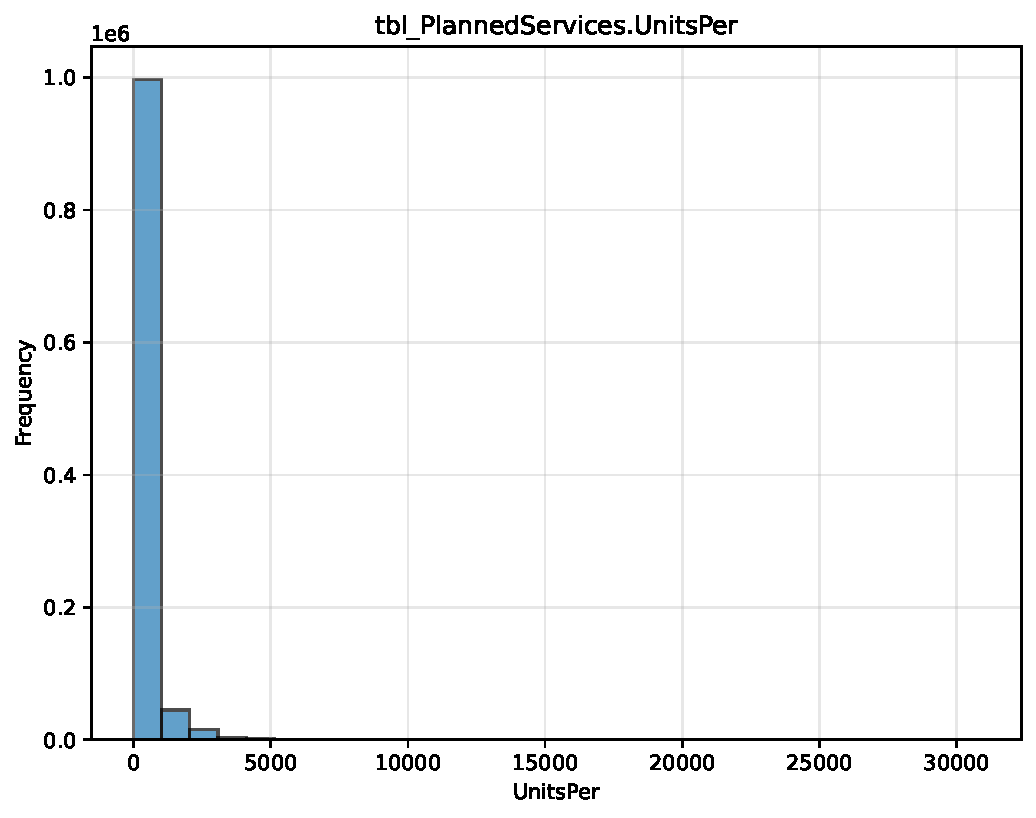
\includegraphics[width=\textwidth]{figures/dbo_tbl_PlannedServices_UnitsPer.pdf}
\caption{Distribution of UnitsPer in tbl\_PlannedServices}
\end{figure}\newpage

\subsection{tbl\_PlannedServices.TotalUnits}
\textit{Total Units}

\begin{figure}[htbp]
\centering
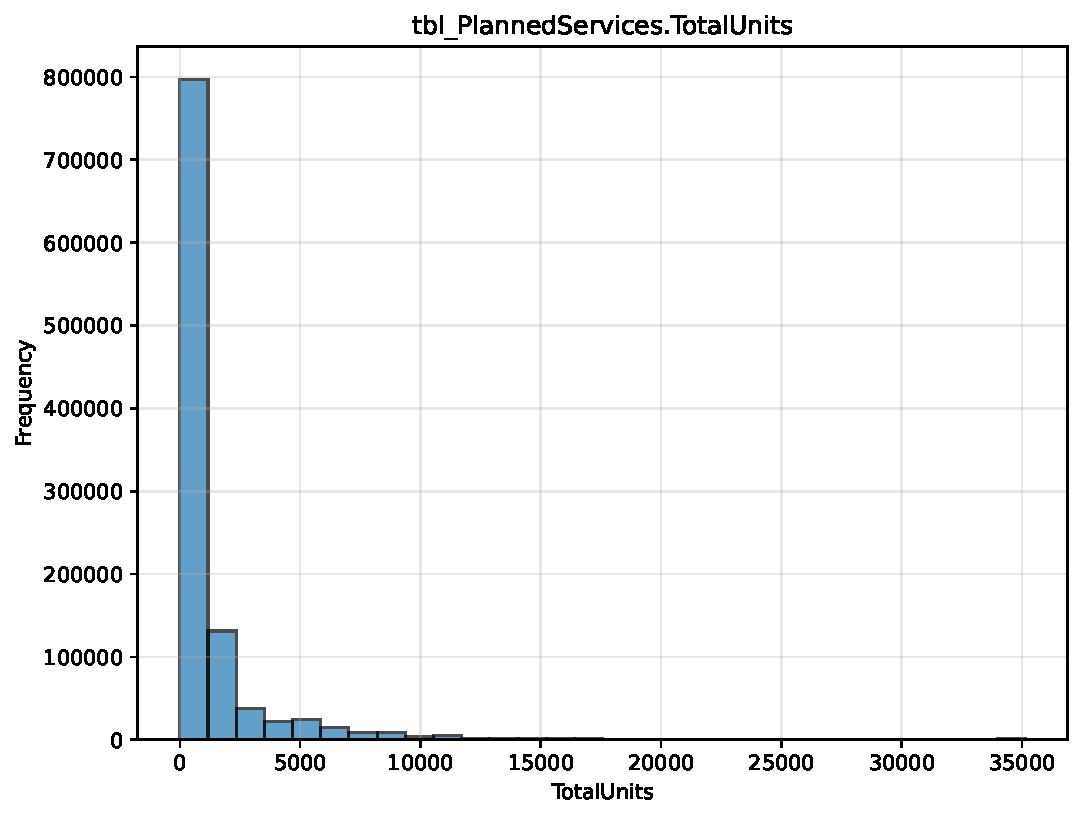
\includegraphics[width=\textwidth]{figures/dbo_tbl_PlannedServices_TotalUnits.pdf}
\caption{Distribution of TotalUnits in tbl\_PlannedServices}
\end{figure}\newpage

\subsection{tbl\_PlannedServices.AnnualizedUnits}
\textit{Annualized Units}

\begin{figure}[htbp]
\centering
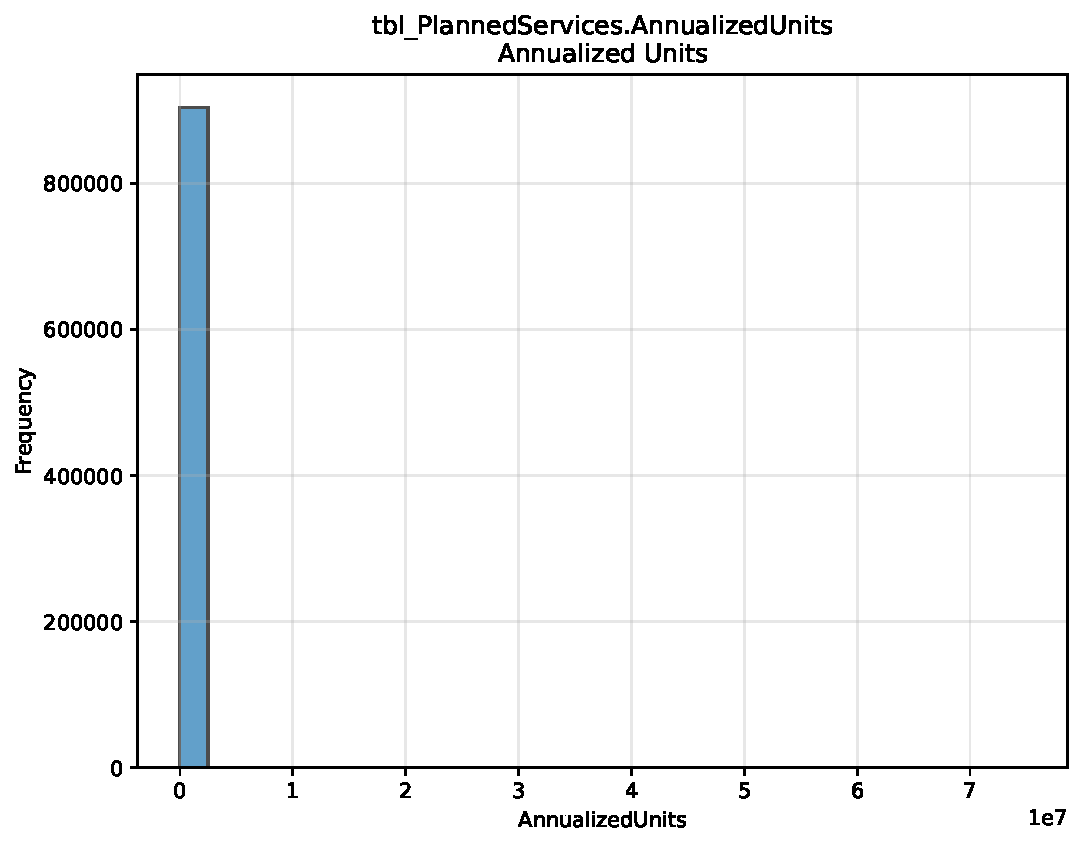
\includegraphics[width=\textwidth]{figures/dbo_tbl_PlannedServices_AnnualizedUnits.pdf}
\caption{Distribution of AnnualizedUnits in tbl\_PlannedServices}
\end{figure}\newpage

\subsection{tbl\_PlannedServices.VendorID}
\textit{Vendor ID (Provider iConnect ID)}

\begin{figure}[htbp]
\centering
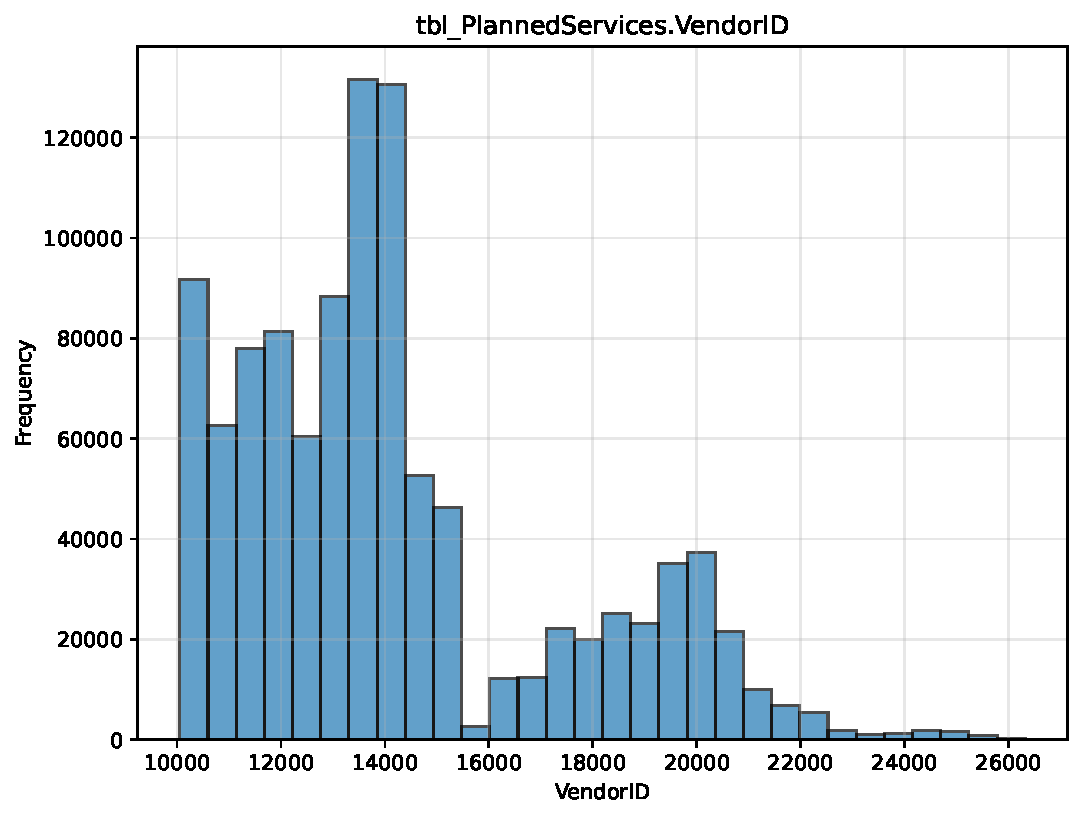
\includegraphics[width=\textwidth]{figures/dbo_tbl_PlannedServices_VendorID.pdf}
\caption{Distribution of VendorID in tbl\_PlannedServices}
\end{figure}\newpage

\subsection{tbl\_PlannedServices.Rate}
\textit{Rate}

\begin{figure}[htbp]
\centering
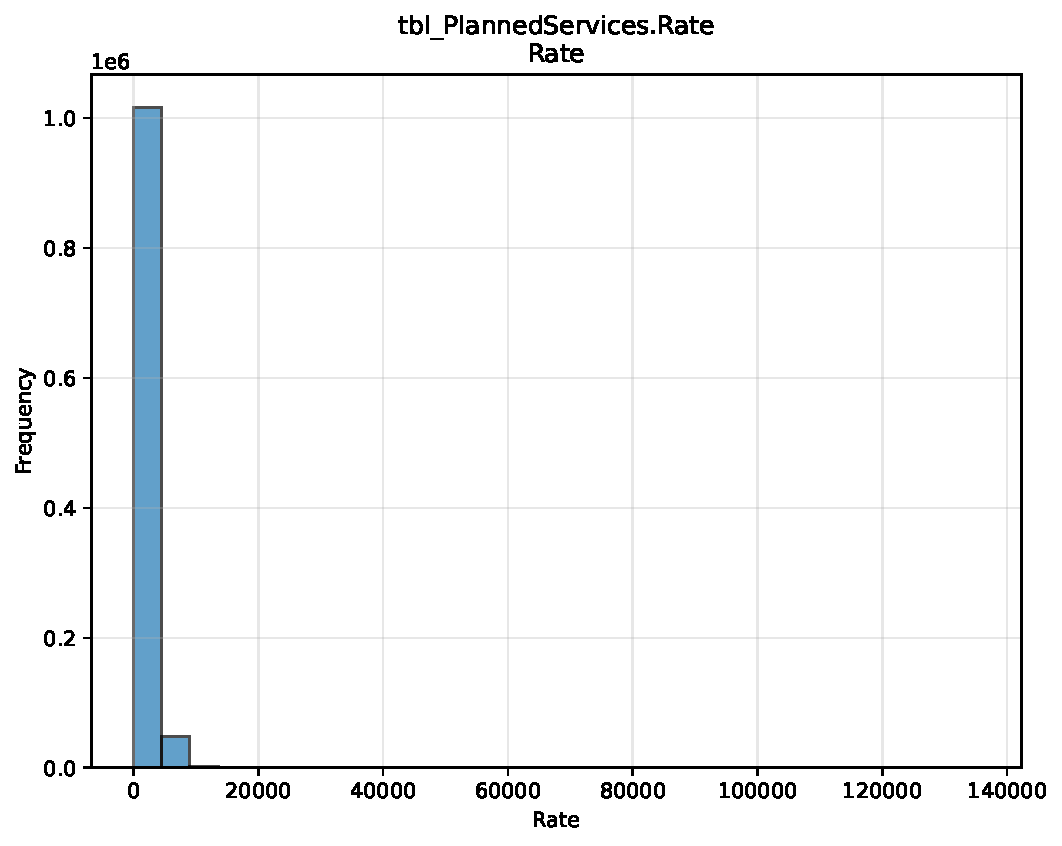
\includegraphics[width=\textwidth]{figures/dbo_tbl_PlannedServices_Rate.pdf}
\caption{Distribution of Rate in tbl\_PlannedServices}
\end{figure}\newpage

\subsection{tbl\_PlannedServices.MaxAmount}
\textit{MaxAmount}

\begin{figure}[htbp]
\centering
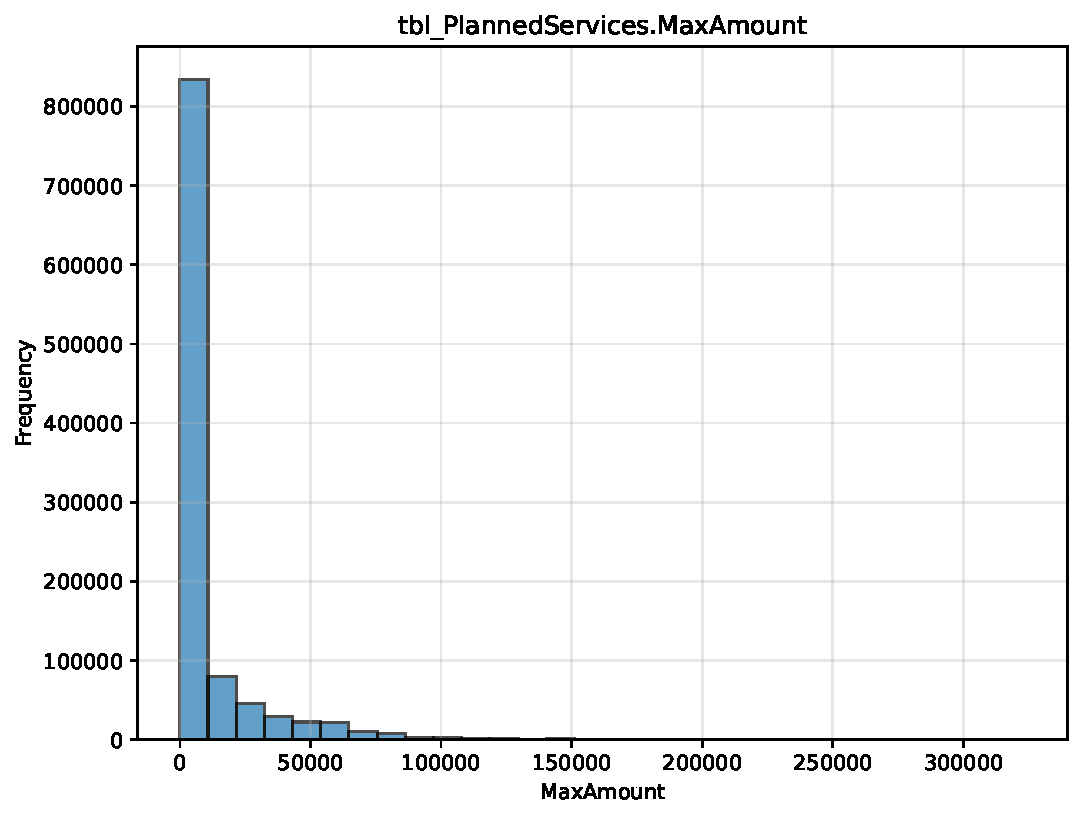
\includegraphics[width=\textwidth]{figures/dbo_tbl_PlannedServices_MaxAmount.pdf}
\caption{Distribution of MaxAmount in tbl\_PlannedServices}
\end{figure}\newpage

\subsection{tbl\_PlannedServices.AllowEVVDelivery}
\textit{Allow EVV Delivery}

\begin{figure}[htbp]
\centering
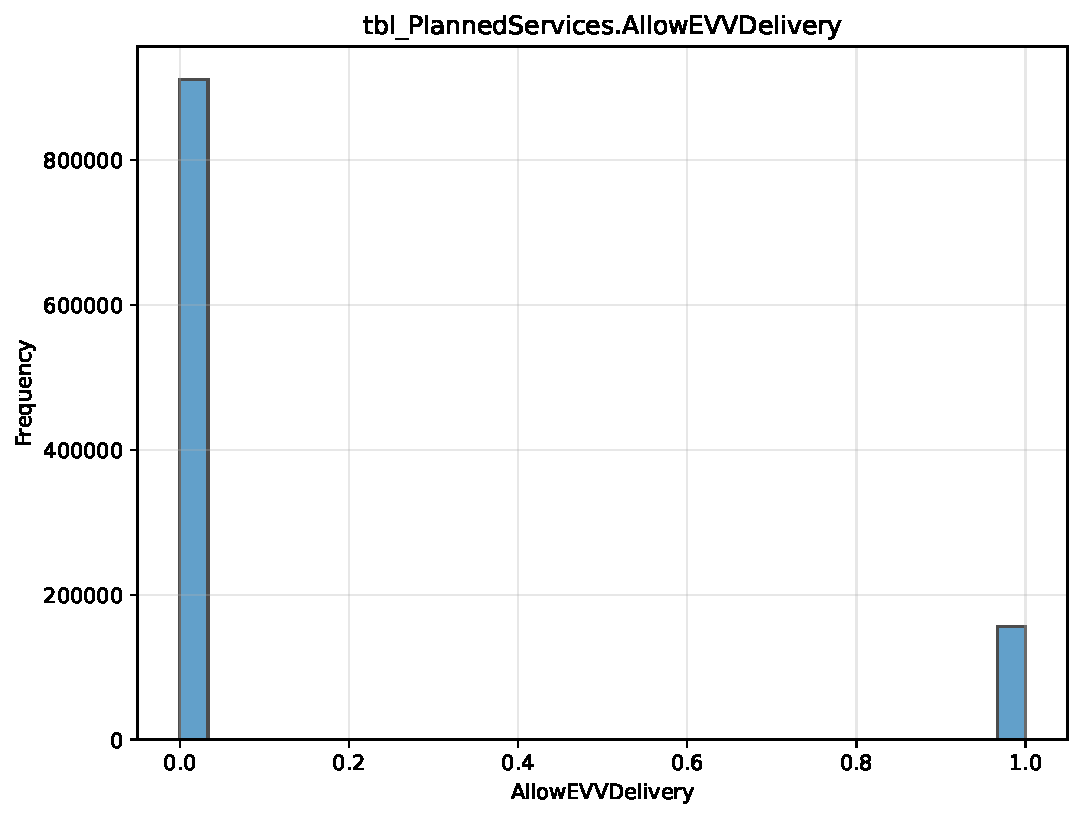
\includegraphics[width=\textwidth]{figures/dbo_tbl_PlannedServices_AllowEVVDelivery.pdf}
\caption{Distribution of AllowEVVDelivery in tbl\_PlannedServices}
\end{figure}\newpage

\subsection{tbl\_PlannedServices.PlannedServiceId}
\textit{Planned Service ID}

\begin{figure}[htbp]
\centering
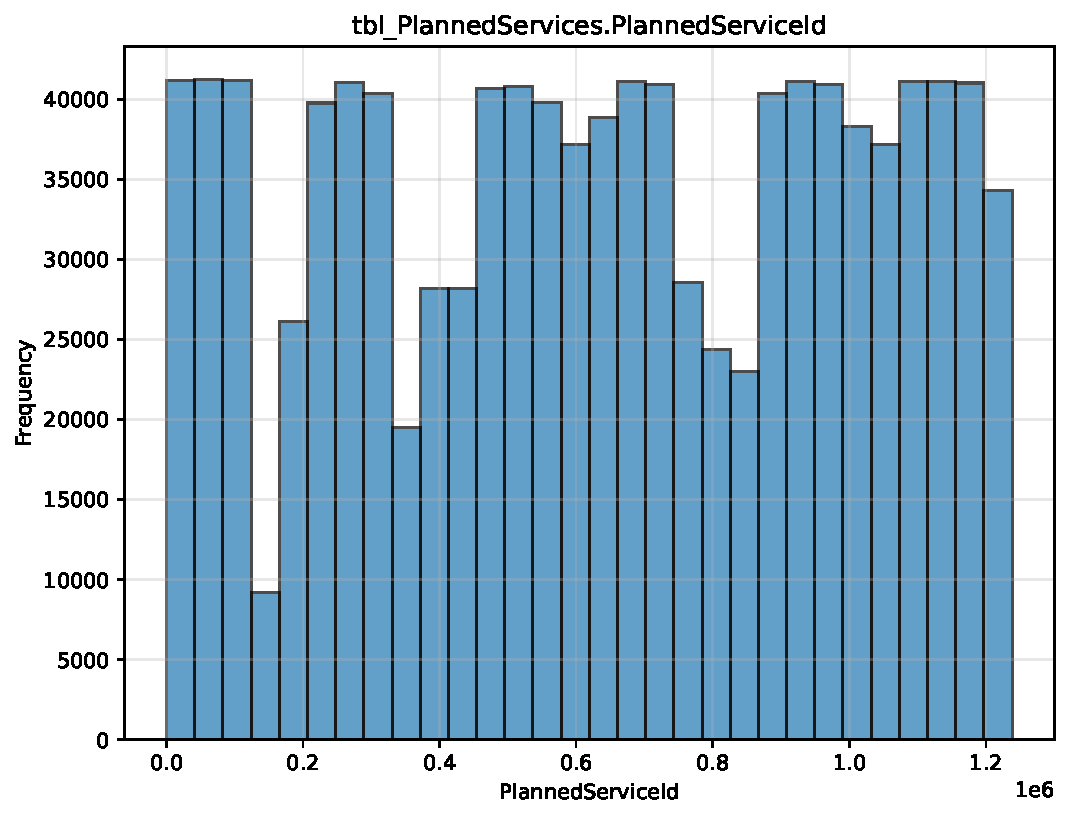
\includegraphics[width=\textwidth]{figures/dbo_tbl_PlannedServices_PlannedServiceId.pdf}
\caption{Distribution of PlannedServiceId in tbl\_PlannedServices}
\end{figure}\newpage

\subsection{tbl\_PlannedServices.PlanId}
\textit{Plan ID}

\begin{figure}[htbp]
\centering
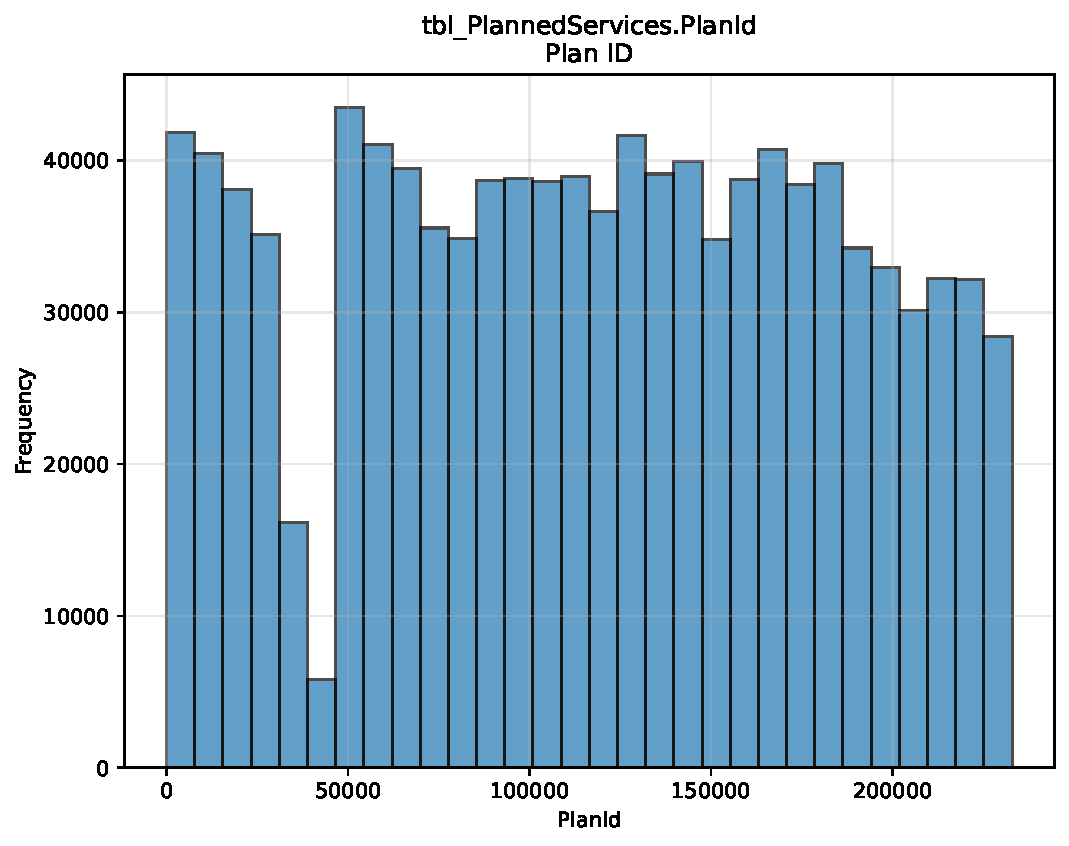
\includegraphics[width=\textwidth]{figures/dbo_tbl_PlannedServices_PlanId.pdf}
\caption{Distribution of PlanId in tbl\_PlannedServices}
\end{figure}\newpage

\subsection{tbl\_PlannedServices.ISComboCodeID}
\textit{IS Combo CodeID}

\begin{figure}[htbp]
\centering
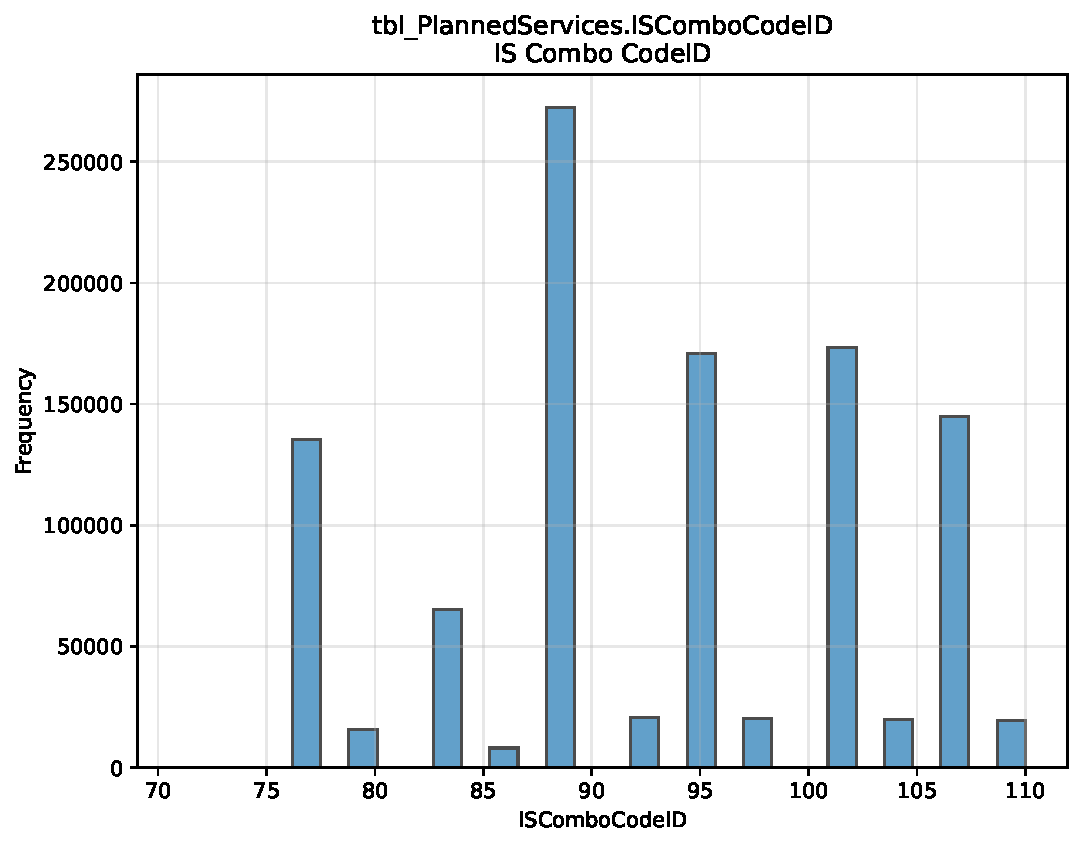
\includegraphics[width=\textwidth]{figures/dbo_tbl_PlannedServices_ISComboCodeID.pdf}
\caption{Distribution of ISComboCodeID in tbl\_PlannedServices}
\end{figure}\newpage

\subsection{tbl\_PlannedServices.VendorServicesId}
\textit{Vendor Services ID}

\begin{figure}[htbp]
\centering
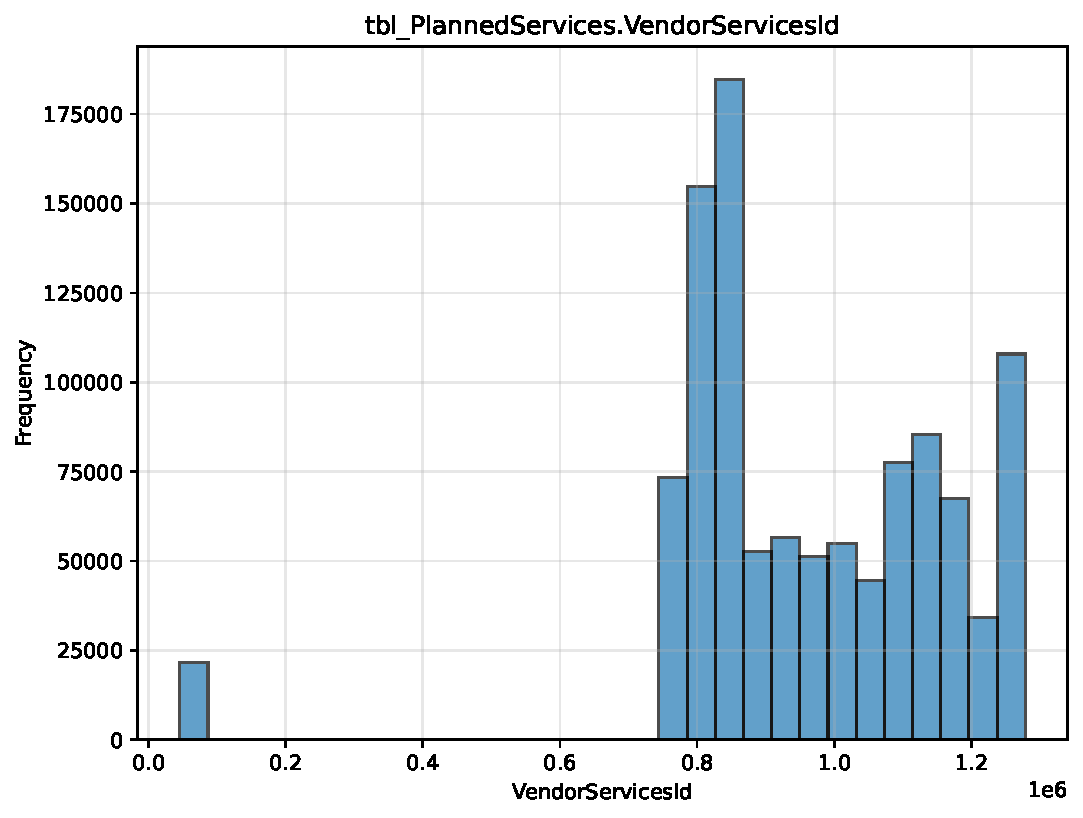
\includegraphics[width=\textwidth]{figures/dbo_tbl_PlannedServices_VendorServicesId.pdf}
\caption{Distribution of VendorServicesId in tbl\_PlannedServices}
\end{figure}\newpage

\subsection{tbl\_Plans.CaseNo}
\textit{Consumer iConnect ID}

\begin{figure}[htbp]
\centering
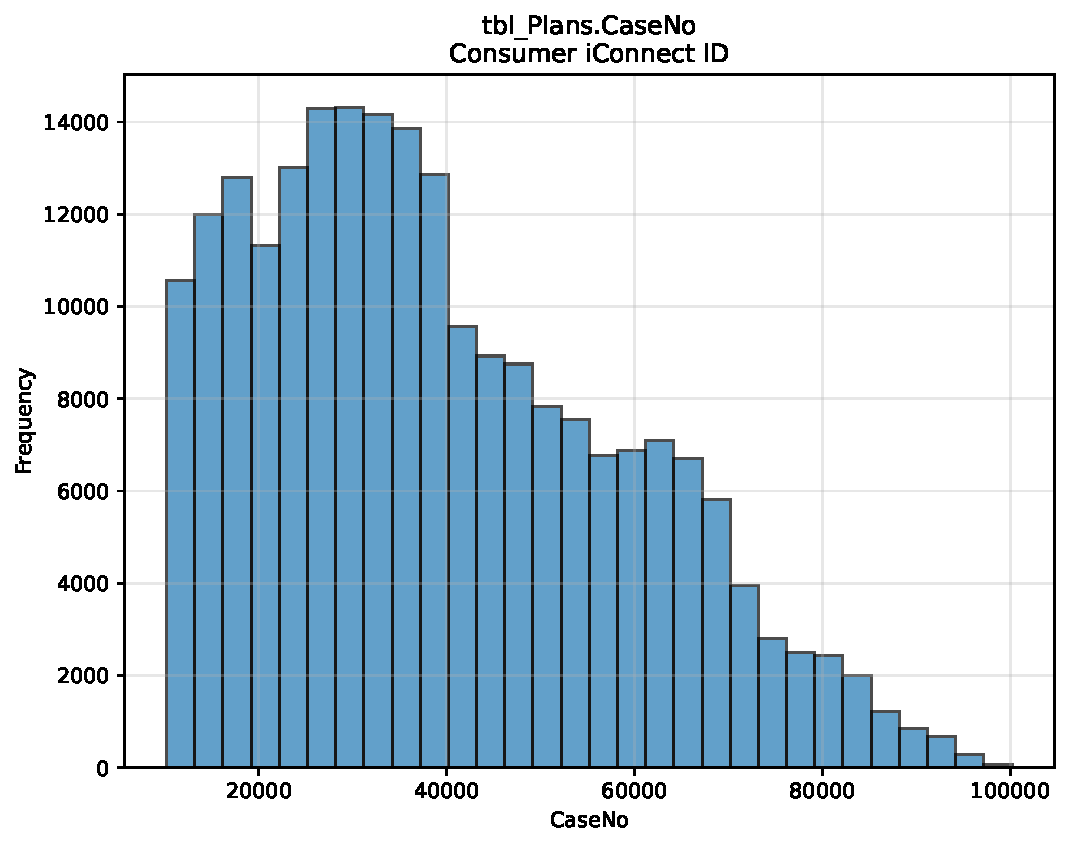
\includegraphics[width=\textwidth]{figures/dbo_tbl_Plans_CaseNo.pdf}
\caption{Distribution of CaseNo in tbl\_Plans}
\end{figure}\newpage

\subsection{tbl\_Plans.PlanId}
\textit{Plan ID}

\begin{figure}[htbp]
\centering
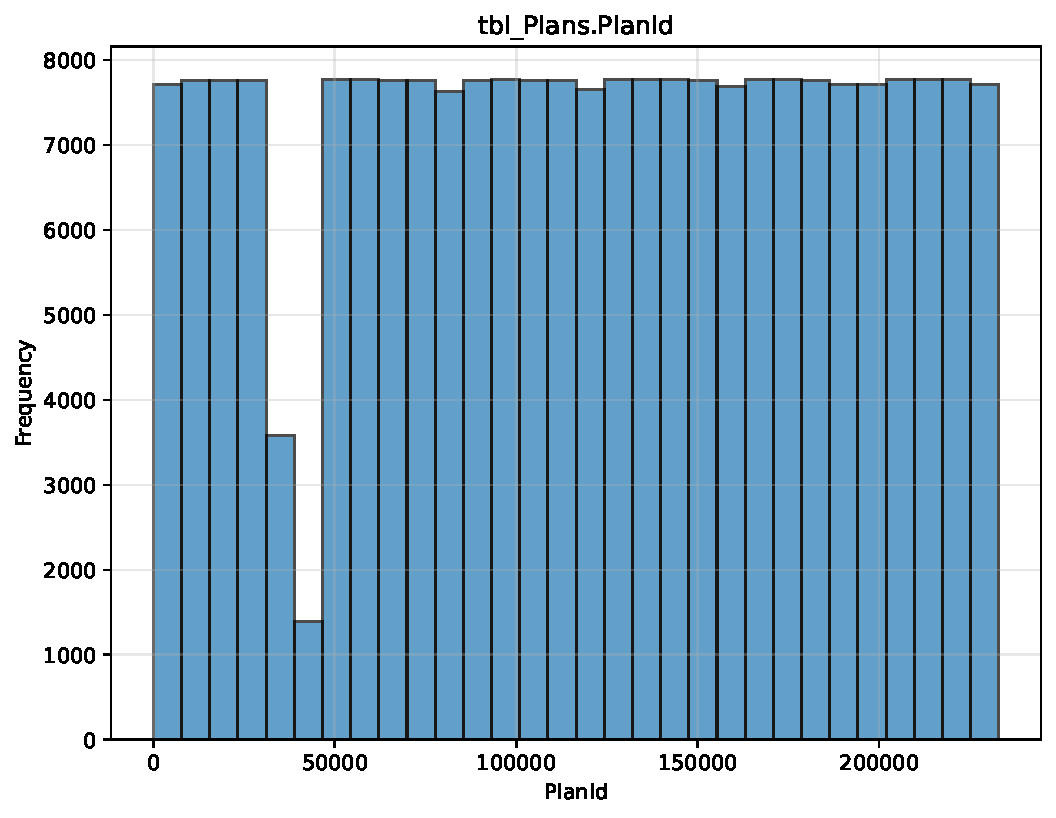
\includegraphics[width=\textwidth]{figures/dbo_tbl_Plans_PlanId.pdf}
\caption{Distribution of PlanId in tbl\_Plans}
\end{figure}\newpage

\subsection{tbl\_Plans.BudgetId}
\textit{Budget ID}

\begin{figure}[htbp]
\centering
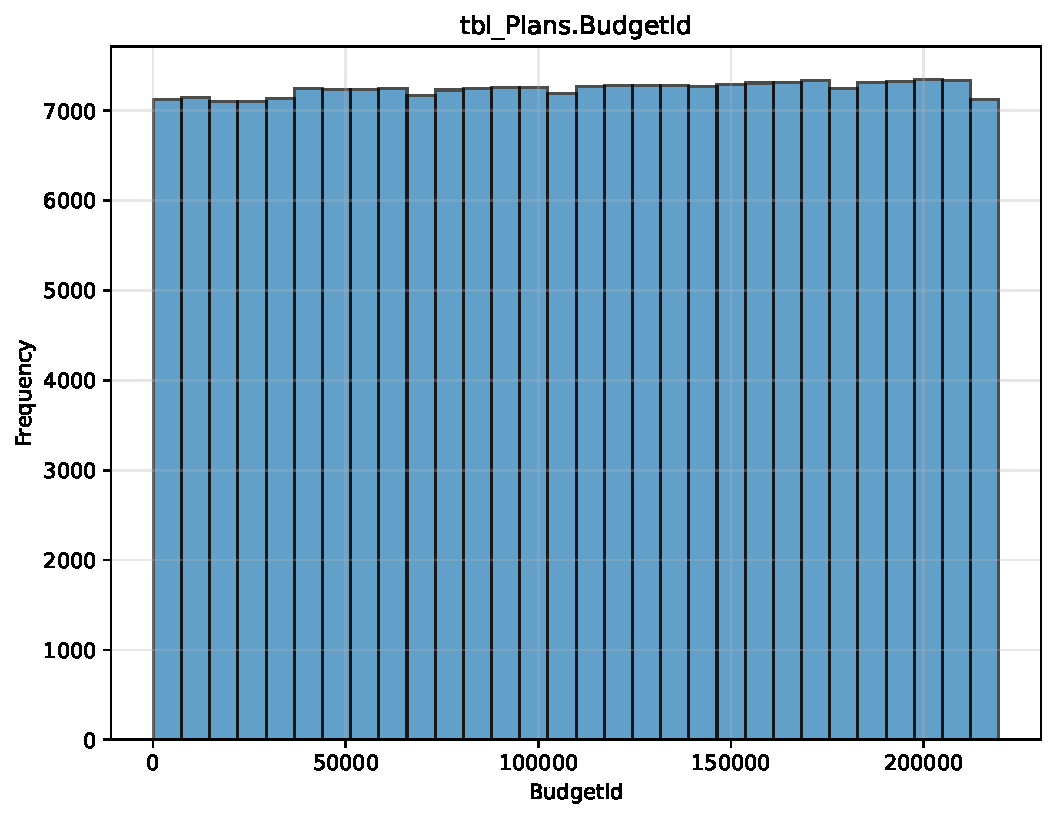
\includegraphics[width=\textwidth]{figures/dbo_tbl_Plans_BudgetId.pdf}
\caption{Distribution of BudgetId in tbl\_Plans}
\end{figure}\newpage

\subsection{tbl\_Plans.OpenId}
\textit{Open ID}

\begin{figure}[htbp]
\centering
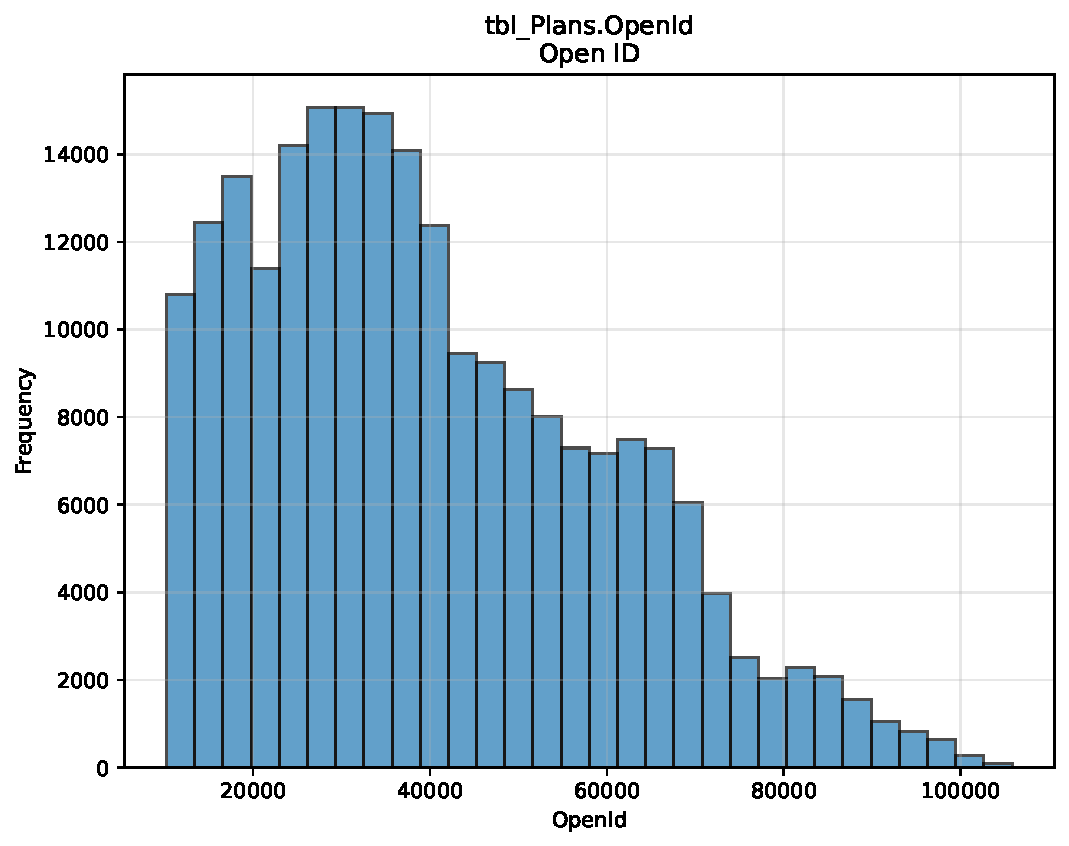
\includegraphics[width=\textwidth]{figures/dbo_tbl_Plans_OpenId.pdf}
\caption{Distribution of OpenId in tbl\_Plans}
\end{figure}\newpage

\subsection{tbl\_Plans.EnrollID}
\textit{Enrollment ID (Program ID)}

\begin{figure}[htbp]
\centering
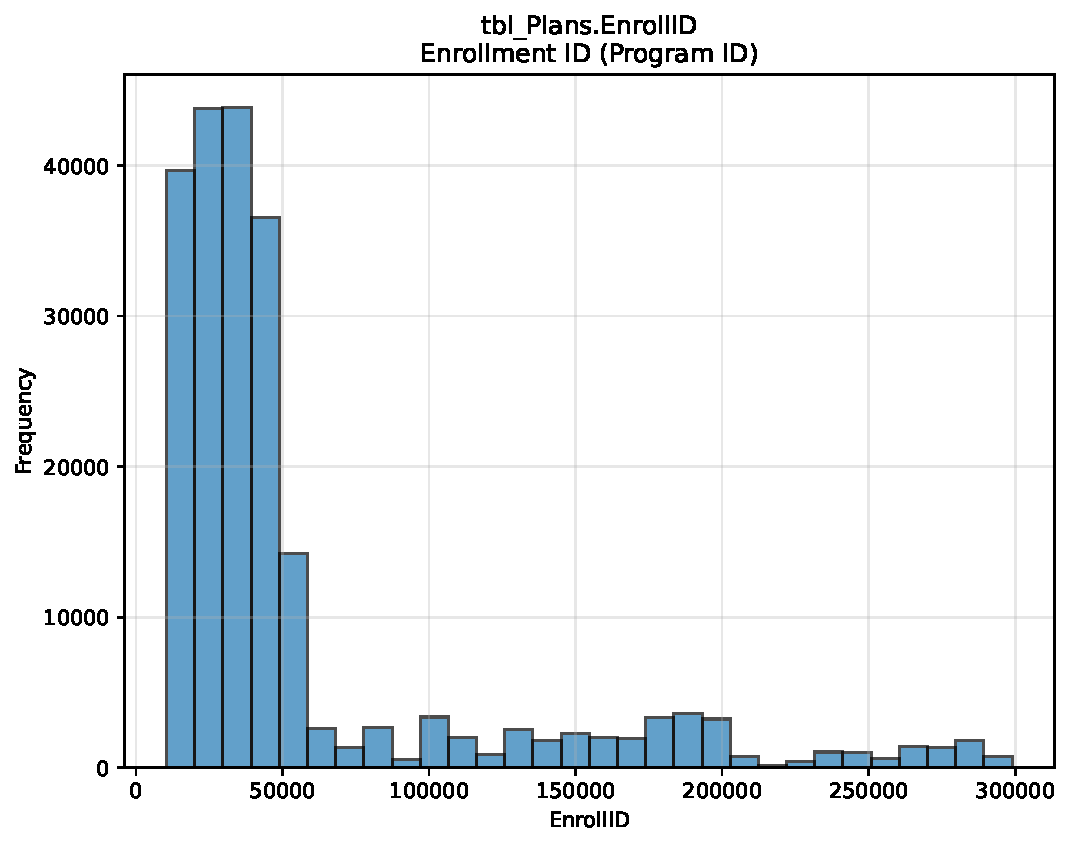
\includegraphics[width=\textwidth]{figures/dbo_tbl_Plans_EnrollID.pdf}
\caption{Distribution of EnrollID in tbl\_Plans}
\end{figure}\newpage

\subsection{tbl\_QSIAssessments.CASENO}
\textit{Consumer iConnect ID}

\begin{figure}[htbp]
\centering
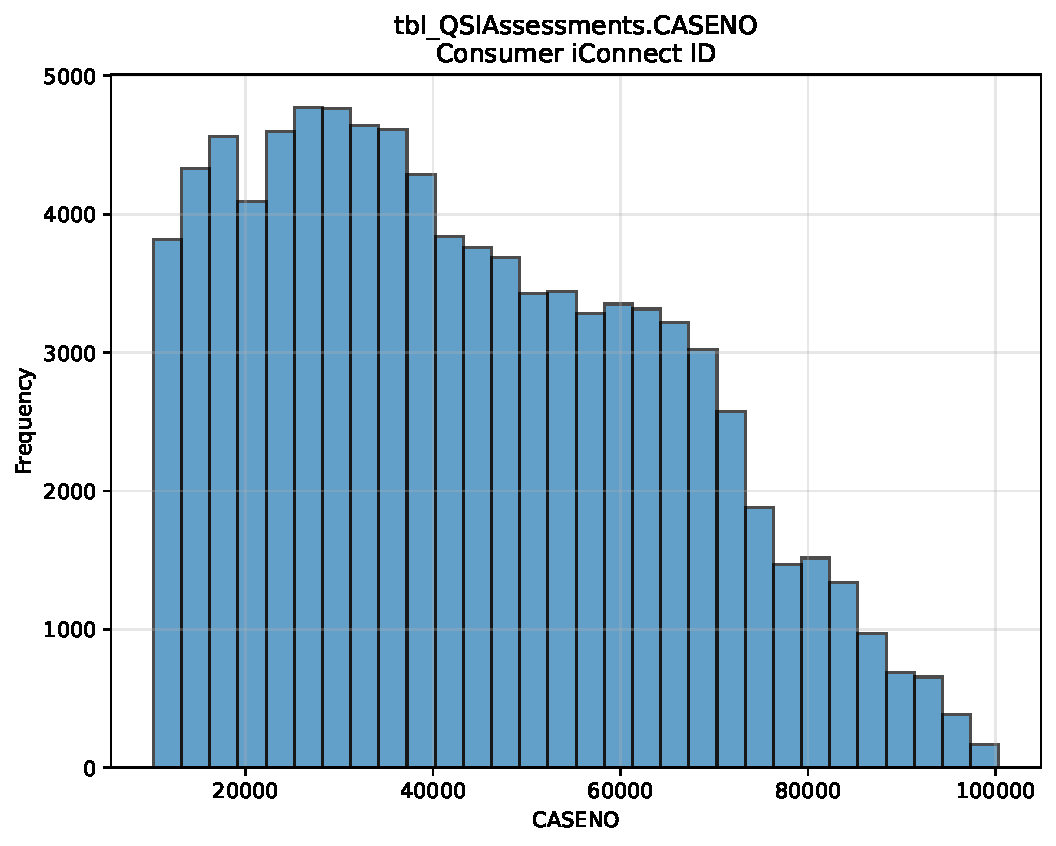
\includegraphics[width=\textwidth]{figures/dbo_tbl_QSIAssessments_CASENO.pdf}
\caption{Distribution of CASENO in tbl\_QSIAssessments}
\end{figure}\newpage

\subsection{tbl\_QSIAssessments.RaterID}
\textit{Rater ID}

\begin{figure}[htbp]
\centering
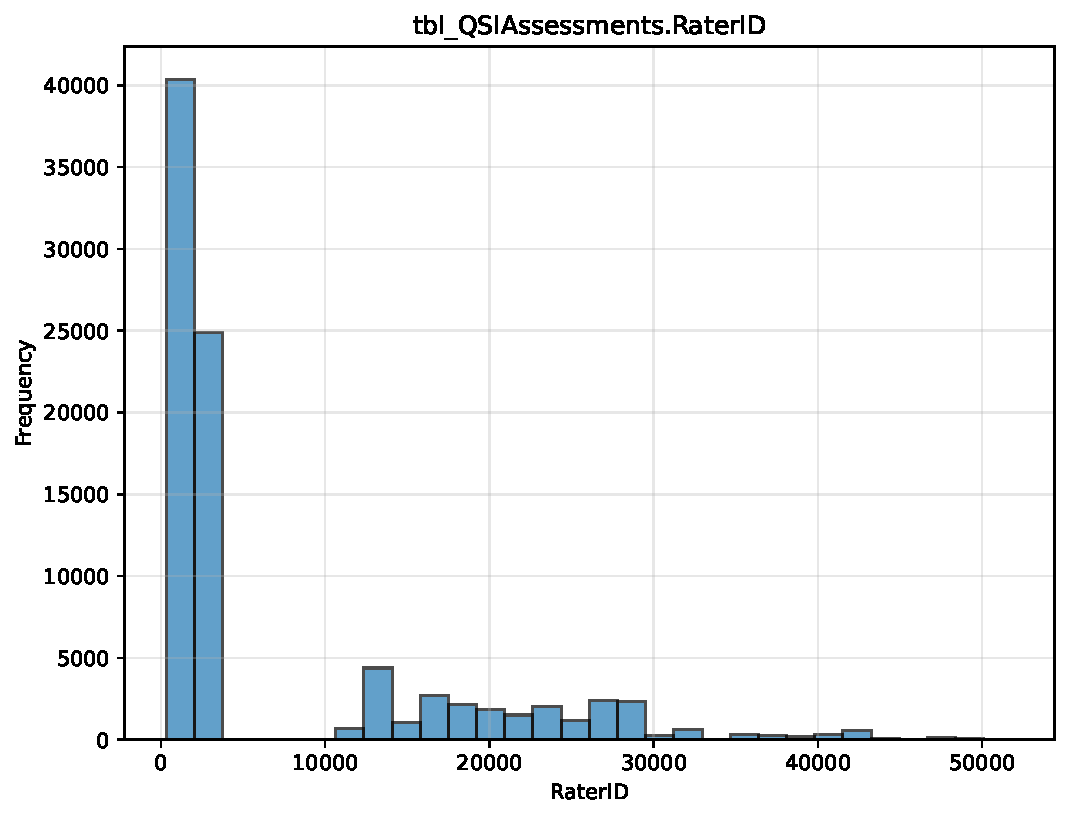
\includegraphics[width=\textwidth]{figures/dbo_tbl_QSIAssessments_RaterID.pdf}
\caption{Distribution of RaterID in tbl\_QSIAssessments}
\end{figure}\newpage

\subsection{tbl\_QSIAssessments.AssessID}
\textit{QSI Assessment Form ID}

\begin{figure}[htbp]
\centering
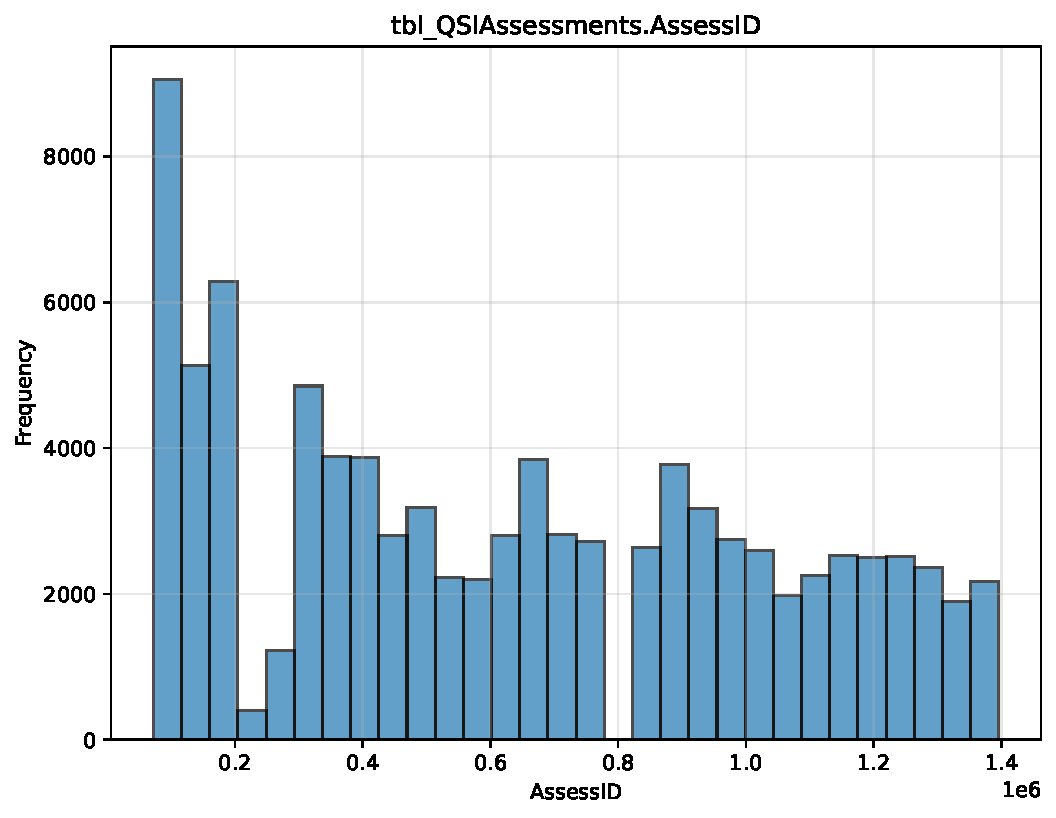
\includegraphics[width=\textwidth]{figures/dbo_tbl_QSIAssessments_AssessID.pdf}
\caption{Distribution of AssessID in tbl\_QSIAssessments}
\end{figure}\newpage

\subsection{tbl\_QSIAssessments.LegacyAssessID}
\textit{Legacy QSI Assessment ID}

\begin{figure}[htbp]
\centering
\includegraphics[width=\textwidth]{figures/dbo_tbl_QSIAssessments_LegacyAssessID.pdf}
\caption{Distribution of LegacyAssessID in tbl\_QSIAssessments}
\end{figure}\newpage

\subsection{tbl\_QSIAssessmentsLegacy.RATERID}
\textit{Rater ID}

\begin{figure}[htbp]
\centering
\includegraphics[width=\textwidth]{figures/dbo_tbl_QSIAssessmentsLegacy_RATERID.pdf}
\caption{Distribution of RATERID in tbl\_QSIAssessmentsLegacy}
\end{figure}\newpage

\subsection{tbl\_QSIAssessmentsLegacy.Q14}
\textit{QSI Question 14}

\begin{figure}[htbp]
\centering
\includegraphics[width=\textwidth]{figures/dbo_tbl_QSIAssessmentsLegacy_Q14.pdf}
\caption{Distribution of Q14 in tbl\_QSIAssessmentsLegacy}
\end{figure}\newpage

\subsection{tbl\_QSIAssessmentsLegacy.Q15}
\textit{QSI Question 15}

\begin{figure}[htbp]
\centering
\includegraphics[width=\textwidth]{figures/dbo_tbl_QSIAssessmentsLegacy_Q15.pdf}
\caption{Distribution of Q15 in tbl\_QSIAssessmentsLegacy}
\end{figure}\newpage

\subsection{tbl\_QSIAssessmentsLegacy.Q16}
\textit{QSI Question 16}

\begin{figure}[htbp]
\centering
\includegraphics[width=\textwidth]{figures/dbo_tbl_QSIAssessmentsLegacy_Q16.pdf}
\caption{Distribution of Q16 in tbl\_QSIAssessmentsLegacy}
\end{figure}\newpage

\subsection{tbl\_QSIAssessmentsLegacy.Q17}
\textit{QSI Question 17}

\begin{figure}[htbp]
\centering
\includegraphics[width=\textwidth]{figures/dbo_tbl_QSIAssessmentsLegacy_Q17.pdf}
\caption{Distribution of Q17 in tbl\_QSIAssessmentsLegacy}
\end{figure}\newpage

\subsection{tbl\_QSIAssessmentsLegacy.Q18}
\textit{QSI Question 18}

\begin{figure}[htbp]
\centering
\includegraphics[width=\textwidth]{figures/dbo_tbl_QSIAssessmentsLegacy_Q18.pdf}
\caption{Distribution of Q18 in tbl\_QSIAssessmentsLegacy}
\end{figure}\newpage

\subsection{tbl\_QSIAssessmentsLegacy.Q19}
\textit{QSI Question 19}

\begin{figure}[htbp]
\centering
\includegraphics[width=\textwidth]{figures/dbo_tbl_QSIAssessmentsLegacy_Q19.pdf}
\caption{Distribution of Q19 in tbl\_QSIAssessmentsLegacy}
\end{figure}\newpage

\subsection{tbl\_QSIAssessmentsLegacy.Q20}
\textit{QSI Question 20}

\begin{figure}[htbp]
\centering
\includegraphics[width=\textwidth]{figures/dbo_tbl_QSIAssessmentsLegacy_Q20.pdf}
\caption{Distribution of Q20 in tbl\_QSIAssessmentsLegacy}
\end{figure}\newpage

\subsection{tbl\_QSIAssessmentsLegacy.Q21}
\textit{QSI Question 21}

\begin{figure}[htbp]
\centering
\includegraphics[width=\textwidth]{figures/dbo_tbl_QSIAssessmentsLegacy_Q21.pdf}
\caption{Distribution of Q21 in tbl\_QSIAssessmentsLegacy}
\end{figure}\newpage

\subsection{tbl\_QSIAssessmentsLegacy.Q22}
\textit{QSI Question 22}

\begin{figure}[htbp]
\centering
\includegraphics[width=\textwidth]{figures/dbo_tbl_QSIAssessmentsLegacy_Q22.pdf}
\caption{Distribution of Q22 in tbl\_QSIAssessmentsLegacy}
\end{figure}\newpage

\subsection{tbl\_QSIAssessmentsLegacy.Q23}
\textit{QSI Question 23}

\begin{figure}[htbp]
\centering
\includegraphics[width=\textwidth]{figures/dbo_tbl_QSIAssessmentsLegacy_Q23.pdf}
\caption{Distribution of Q23 in tbl\_QSIAssessmentsLegacy}
\end{figure}\newpage

\subsection{tbl\_QSIAssessmentsLegacy.Q24}
\textit{QSI Question 24}

\begin{figure}[htbp]
\centering
\includegraphics[width=\textwidth]{figures/dbo_tbl_QSIAssessmentsLegacy_Q24.pdf}
\caption{Distribution of Q24 in tbl\_QSIAssessmentsLegacy}
\end{figure}\newpage

\subsection{tbl\_QSIAssessmentsLegacy.Q25}
\textit{QSI Question 25}

\begin{figure}[htbp]
\centering
\includegraphics[width=\textwidth]{figures/dbo_tbl_QSIAssessmentsLegacy_Q25.pdf}
\caption{Distribution of Q25 in tbl\_QSIAssessmentsLegacy}
\end{figure}\newpage

\subsection{tbl\_QSIAssessmentsLegacy.Q26}
\textit{QSI Question 26}

\begin{figure}[htbp]
\centering
\includegraphics[width=\textwidth]{figures/dbo_tbl_QSIAssessmentsLegacy_Q26.pdf}
\caption{Distribution of Q26 in tbl\_QSIAssessmentsLegacy}
\end{figure}\newpage

\subsection{tbl\_QSIAssessmentsLegacy.Q27}
\textit{QSI Question 27}

\begin{figure}[htbp]
\centering
\includegraphics[width=\textwidth]{figures/dbo_tbl_QSIAssessmentsLegacy_Q27.pdf}
\caption{Distribution of Q27 in tbl\_QSIAssessmentsLegacy}
\end{figure}\newpage

\subsection{tbl\_QSIAssessmentsLegacy.Q28}
\textit{QSI Question 28}

\begin{figure}[htbp]
\centering
\includegraphics[width=\textwidth]{figures/dbo_tbl_QSIAssessmentsLegacy_Q28.pdf}
\caption{Distribution of Q28 in tbl\_QSIAssessmentsLegacy}
\end{figure}\newpage

\subsection{tbl\_QSIAssessmentsLegacy.Q29}
\textit{QSI Question 29}

\begin{figure}[htbp]
\centering
\includegraphics[width=\textwidth]{figures/dbo_tbl_QSIAssessmentsLegacy_Q29.pdf}
\caption{Distribution of Q29 in tbl\_QSIAssessmentsLegacy}
\end{figure}\newpage

\subsection{tbl\_QSIAssessmentsLegacy.Q30}
\textit{QSI Question 30}

\begin{figure}[htbp]
\centering
\includegraphics[width=\textwidth]{figures/dbo_tbl_QSIAssessmentsLegacy_Q30.pdf}
\caption{Distribution of Q30 in tbl\_QSIAssessmentsLegacy}
\end{figure}\newpage

\subsection{tbl\_QSIAssessmentsLegacy.Q30a}
\textit{QSI Question 30a}

\begin{figure}[htbp]
\centering
\includegraphics[width=\textwidth]{figures/dbo_tbl_QSIAssessmentsLegacy_Q30a.pdf}
\caption{Distribution of Q30a in tbl\_QSIAssessmentsLegacy}
\end{figure}\newpage

\subsection{tbl\_QSIAssessmentsLegacy.Q30b}
\textit{QSI Question 30b}

\begin{figure}[htbp]
\centering
\includegraphics[width=\textwidth]{figures/dbo_tbl_QSIAssessmentsLegacy_Q30b.pdf}
\caption{Distribution of Q30b in tbl\_QSIAssessmentsLegacy}
\end{figure}\newpage

\subsection{tbl\_QSIAssessmentsLegacy.Q31}
\textit{QSI Question 31}

\begin{figure}[htbp]
\centering
\includegraphics[width=\textwidth]{figures/dbo_tbl_QSIAssessmentsLegacy_Q31.pdf}
\caption{Distribution of Q31 in tbl\_QSIAssessmentsLegacy}
\end{figure}\newpage

\subsection{tbl\_QSIAssessmentsLegacy.Q32}
\textit{QSI Question 32}

\begin{figure}[htbp]
\centering
\includegraphics[width=\textwidth]{figures/dbo_tbl_QSIAssessmentsLegacy_Q32.pdf}
\caption{Distribution of Q32 in tbl\_QSIAssessmentsLegacy}
\end{figure}\newpage

\subsection{tbl\_QSIAssessmentsLegacy.Q33}
\textit{QSI Question 33}

\begin{figure}[htbp]
\centering
\includegraphics[width=\textwidth]{figures/dbo_tbl_QSIAssessmentsLegacy_Q33.pdf}
\caption{Distribution of Q33 in tbl\_QSIAssessmentsLegacy}
\end{figure}\newpage

\subsection{tbl\_QSIAssessmentsLegacy.Q34}
\textit{QSI Question 34}

\begin{figure}[htbp]
\centering
\includegraphics[width=\textwidth]{figures/dbo_tbl_QSIAssessmentsLegacy_Q34.pdf}
\caption{Distribution of Q34 in tbl\_QSIAssessmentsLegacy}
\end{figure}\newpage

\subsection{tbl\_QSIAssessmentsLegacy.Q35}
\textit{QSI Question 35}

\begin{figure}[htbp]
\centering
\includegraphics[width=\textwidth]{figures/dbo_tbl_QSIAssessmentsLegacy_Q35.pdf}
\caption{Distribution of Q35 in tbl\_QSIAssessmentsLegacy}
\end{figure}\newpage

\subsection{tbl\_QSIAssessmentsLegacy.Q36}
\textit{QSI Question 36}

\begin{figure}[htbp]
\centering
\includegraphics[width=\textwidth]{figures/dbo_tbl_QSIAssessmentsLegacy_Q36.pdf}
\caption{Distribution of Q36 in tbl\_QSIAssessmentsLegacy}
\end{figure}\newpage

\subsection{tbl\_QSIAssessmentsLegacy.Q37}
\textit{QSI Quesiton 37}

\begin{figure}[htbp]
\centering
\includegraphics[width=\textwidth]{figures/dbo_tbl_QSIAssessmentsLegacy_Q37.pdf}
\caption{Distribution of Q37 in tbl\_QSIAssessmentsLegacy}
\end{figure}\newpage

\subsection{tbl\_QSIAssessmentsLegacy.Q38}
\textit{QSI Question 38}

\begin{figure}[htbp]
\centering
\includegraphics[width=\textwidth]{figures/dbo_tbl_QSIAssessmentsLegacy_Q38.pdf}
\caption{Distribution of Q38 in tbl\_QSIAssessmentsLegacy}
\end{figure}\newpage

\subsection{tbl\_QSIAssessmentsLegacy.Q39}
\textit{QSI Question 39}

\begin{figure}[htbp]
\centering
\includegraphics[width=\textwidth]{figures/dbo_tbl_QSIAssessmentsLegacy_Q39.pdf}
\caption{Distribution of Q39 in tbl\_QSIAssessmentsLegacy}
\end{figure}\newpage

\subsection{tbl\_QSIAssessmentsLegacy.Q40}
\textit{QSI Question 40}

\begin{figure}[htbp]
\centering
\includegraphics[width=\textwidth]{figures/dbo_tbl_QSIAssessmentsLegacy_Q40.pdf}
\caption{Distribution of Q40 in tbl\_QSIAssessmentsLegacy}
\end{figure}\newpage

\subsection{tbl\_QSIAssessmentsLegacy.Q41}
\textit{QSI Question 41}

\begin{figure}[htbp]
\centering
\includegraphics[width=\textwidth]{figures/dbo_tbl_QSIAssessmentsLegacy_Q41.pdf}
\caption{Distribution of Q41 in tbl\_QSIAssessmentsLegacy}
\end{figure}\newpage

\subsection{tbl\_QSIAssessmentsLegacy.Q42}
\textit{QSI Question 42}

\begin{figure}[htbp]
\centering
\includegraphics[width=\textwidth]{figures/dbo_tbl_QSIAssessmentsLegacy_Q42.pdf}
\caption{Distribution of Q42 in tbl\_QSIAssessmentsLegacy}
\end{figure}\newpage

\subsection{tbl\_QSIAssessmentsLegacy.Q43}
\textit{QSI Question 43}

\begin{figure}[htbp]
\centering
\includegraphics[width=\textwidth]{figures/dbo_tbl_QSIAssessmentsLegacy_Q43.pdf}
\caption{Distribution of Q43 in tbl\_QSIAssessmentsLegacy}
\end{figure}\newpage

\subsection{tbl\_QSIAssessmentsLegacy.Q44}
\textit{QSI Question 44}

\begin{figure}[htbp]
\centering
\includegraphics[width=\textwidth]{figures/dbo_tbl_QSIAssessmentsLegacy_Q44.pdf}
\caption{Distribution of Q44 in tbl\_QSIAssessmentsLegacy}
\end{figure}\newpage

\subsection{tbl\_QSIAssessmentsLegacy.Q45}
\textit{QSI Question 45}

\begin{figure}[htbp]
\centering
\includegraphics[width=\textwidth]{figures/dbo_tbl_QSIAssessmentsLegacy_Q45.pdf}
\caption{Distribution of Q45 in tbl\_QSIAssessmentsLegacy}
\end{figure}\newpage

\subsection{tbl\_QSIAssessmentsLegacy.Q46}
\textit{QSI Question 46}

\begin{figure}[htbp]
\centering
\includegraphics[width=\textwidth]{figures/dbo_tbl_QSIAssessmentsLegacy_Q46.pdf}
\caption{Distribution of Q46 in tbl\_QSIAssessmentsLegacy}
\end{figure}\newpage

\subsection{tbl\_QSIAssessmentsLegacy.Q47}
\textit{QSI Question 47}

\begin{figure}[htbp]
\centering
\includegraphics[width=\textwidth]{figures/dbo_tbl_QSIAssessmentsLegacy_Q47.pdf}
\caption{Distribution of Q47 in tbl\_QSIAssessmentsLegacy}
\end{figure}\newpage

\subsection{tbl\_QSIAssessmentsLegacy.Q48}
\textit{QSI Question 48}

\begin{figure}[htbp]
\centering
\includegraphics[width=\textwidth]{figures/dbo_tbl_QSIAssessmentsLegacy_Q48.pdf}
\caption{Distribution of Q48 in tbl\_QSIAssessmentsLegacy}
\end{figure}\newpage

\subsection{tbl\_QSIAssessmentsLegacy.Q49}
\textit{QSI Question 49}

\begin{figure}[htbp]
\centering
\includegraphics[width=\textwidth]{figures/dbo_tbl_QSIAssessmentsLegacy_Q49.pdf}
\caption{Distribution of Q49 in tbl\_QSIAssessmentsLegacy}
\end{figure}\newpage

\subsection{tbl\_QSIAssessmentsLegacy.Q49a}
\textit{QSI Question 49a}

\begin{figure}[htbp]
\centering
\includegraphics[width=\textwidth]{figures/dbo_tbl_QSIAssessmentsLegacy_Q49a.pdf}
\caption{Distribution of Q49a in tbl\_QSIAssessmentsLegacy}
\end{figure}\newpage

\subsection{tbl\_QSIAssessmentsLegacy.FLEVEL}
\textit{Functional Level}

\begin{figure}[htbp]
\centering
\includegraphics[width=\textwidth]{figures/dbo_tbl_QSIAssessmentsLegacy_FLEVEL.pdf}
\caption{Distribution of FLEVEL in tbl\_QSIAssessmentsLegacy}
\end{figure}\newpage

\subsection{tbl\_QSIAssessmentsLegacy.BLEVEL}
\textit{Behavioral Level}

\begin{figure}[htbp]
\centering
\includegraphics[width=\textwidth]{figures/dbo_tbl_QSIAssessmentsLegacy_BLEVEL.pdf}
\caption{Distribution of BLEVEL in tbl\_QSIAssessmentsLegacy}
\end{figure}\newpage

\subsection{tbl\_QSIAssessmentsLegacy.PLEVEL}
\textit{Physical Level}

\begin{figure}[htbp]
\centering
\includegraphics[width=\textwidth]{figures/dbo_tbl_QSIAssessmentsLegacy_PLEVEL.pdf}
\caption{Distribution of PLEVEL in tbl\_QSIAssessmentsLegacy}
\end{figure}\newpage

\subsection{tbl\_QSIAssessmentsLegacy.LOSRI}
\textit{Level of Support Rating}

\begin{figure}[htbp]
\centering
\includegraphics[width=\textwidth]{figures/dbo_tbl_QSIAssessmentsLegacy_LOSRI.pdf}
\caption{Distribution of LOSRI in tbl\_QSIAssessmentsLegacy}
\end{figure}\newpage

\subsection{tbl\_QSIAssessmentsLegacy.ASSESSID}
\textit{Assessment ID}

\begin{figure}[htbp]
\centering
\includegraphics[width=\textwidth]{figures/dbo_tbl_QSIAssessmentsLegacy_ASSESSID.pdf}
\caption{Distribution of ASSESSID in tbl\_QSIAssessmentsLegacy}
\end{figure}\newpage

\subsection{tbl\_QSIQuestions.QuestionAssoc}
\textit{Question Association}

\begin{figure}[htbp]
\centering
\includegraphics[width=\textwidth]{figures/dbo_tbl_QSIQuestions_QuestionAssoc.pdf}
\caption{Distribution of QuestionAssoc in tbl\_QSIQuestions}
\end{figure}\newpage

\subsection{tbl\_Rates.UnitCost}

\begin{figure}[htbp]
\centering
\includegraphics[width=\textwidth]{figures/dbo_tbl_Rates_UnitCost.pdf}
\caption{Distribution of UnitCost in tbl\_Rates}
\end{figure}\newpage

\subsection{tbl\_Rates.UserStamp}

\begin{figure}[htbp]
\centering
\includegraphics[width=\textwidth]{figures/dbo_tbl_Rates_UserStamp.pdf}
\caption{Distribution of UserStamp in tbl\_Rates}
\end{figure}\newpage

\subsection{tbl\_Rates.ServiceCodeUnitCostID}

\begin{figure}[htbp]
\centering
\includegraphics[width=\textwidth]{figures/dbo_tbl_Rates_ServiceCodeUnitCostID.pdf}
\caption{Distribution of ServiceCodeUnitCostID in tbl\_Rates}
\end{figure}\newpage

\subsection{tbl\_Rates.ServiceCodesId}

\begin{figure}[htbp]
\centering
\includegraphics[width=\textwidth]{figures/dbo_tbl_Rates_ServiceCodesId.pdf}
\caption{Distribution of ServiceCodesId in tbl\_Rates}
\end{figure}\newpage

\subsection{tbl\_SANs.CaseNo}
\textit{Consumer iConnect ID}

\begin{figure}[htbp]
\centering
\includegraphics[width=\textwidth]{figures/dbo_tbl_SANs_CaseNo.pdf}
\caption{Distribution of CaseNo in tbl\_SANs}
\end{figure}\newpage

\subsection{tbl\_SANs.SanID}
\textit{SAN ID}

\begin{figure}[htbp]
\centering
\includegraphics[width=\textwidth]{figures/dbo_tbl_SANs_SanID.pdf}
\caption{Distribution of SanID in tbl\_SANs}
\end{figure}\newpage

\subsection{tbl\_SANs.PlanID}
\textit{Plan ID}

\begin{figure}[htbp]
\centering
\includegraphics[width=\textwidth]{figures/dbo_tbl_SANs_PlanID.pdf}
\caption{Distribution of PlanID in tbl\_SANs}
\end{figure}\newpage

\subsection{tbl\_SANs.CurrentBudget}
\textit{Current Budget}

\begin{figure}[htbp]
\centering
\includegraphics[width=\textwidth]{figures/dbo_tbl_SANs_CurrentBudget.pdf}
\caption{Distribution of CurrentBudget in tbl\_SANs}
\end{figure}\newpage

\subsection{tbl\_SANs.AlgorithmAmount}
\textit{Algorithm Amount}

\begin{figure}[htbp]
\centering
\includegraphics[width=\textwidth]{figures/dbo_tbl_SANs_AlgorithmAmount.pdf}
\caption{Distribution of AlgorithmAmount in tbl\_SANs}
\end{figure}\newpage

\subsection{tbl\_SANs.AmountUnAuthorized}
\textit{Amoun tUnAuthorized}

\begin{figure}[htbp]
\centering
\includegraphics[width=\textwidth]{figures/dbo_tbl_SANs_AmountUnAuthorized.pdf}
\caption{Distribution of AmountUnAuthorized in tbl\_SANs}
\end{figure}\newpage

\subsection{tbl\_SANs.WSCProposedBudget}
\textit{WSC Proposed Budget}

\begin{figure}[htbp]
\centering
\includegraphics[width=\textwidth]{figures/dbo_tbl_SANs_WSCProposedBudget.pdf}
\caption{Distribution of WSCProposedBudget in tbl\_SANs}
\end{figure}\newpage

\subsection{tbl\_SANs.WSCProposedProratedIncrease}
\textit{WSC Proposed Prorated Increase}

\begin{figure}[htbp]
\centering
\includegraphics[width=\textwidth]{figures/dbo_tbl_SANs_WSCProposedProratedIncrease.pdf}
\caption{Distribution of WSCProposedProratedIncrease in tbl\_SANs}
\end{figure}\newpage

\subsection{tbl\_SANs.WSCProposedAnnualizedBudget}
\textit{WSC Proposed Annualized Budget}

\begin{figure}[htbp]
\centering
\includegraphics[width=\textwidth]{figures/dbo_tbl_SANs_WSCProposedAnnualizedBudget.pdf}
\caption{Distribution of WSCProposedAnnualizedBudget in tbl\_SANs}
\end{figure}\newpage

\subsection{tbl\_SANs.WSCProposedAnnualizedIncrease}
\textit{WSC Proposed Annualized Increase}

\begin{figure}[htbp]
\centering
\includegraphics[width=\textwidth]{figures/dbo_tbl_SANs_WSCProposedAnnualizedIncrease.pdf}
\caption{Distribution of WSCProposedAnnualizedIncrease in tbl\_SANs}
\end{figure}\newpage

\subsection{tbl\_SANs.StateProposedProratedBudget}
\textit{State Proposed Prorated Budget}

\begin{figure}[htbp]
\centering
\includegraphics[width=\textwidth]{figures/dbo_tbl_SANs_StateProposedProratedBudget.pdf}
\caption{Distribution of StateProposedProratedBudget in tbl\_SANs}
\end{figure}\newpage

\subsection{tbl\_SANs.StateProposedProratedIncrease}
\textit{State Proposed Prorated Increase}

\begin{figure}[htbp]
\centering
\includegraphics[width=\textwidth]{figures/dbo_tbl_SANs_StateProposedProratedIncrease.pdf}
\caption{Distribution of StateProposedProratedIncrease in tbl\_SANs}
\end{figure}\newpage

\subsection{tbl\_SANs.StateProposedAnnualizedBudget}
\textit{State Proposed Annualized Budget}

\begin{figure}[htbp]
\centering
\includegraphics[width=\textwidth]{figures/dbo_tbl_SANs_StateProposedAnnualizedBudget.pdf}
\caption{Distribution of StateProposedAnnualizedBudget in tbl\_SANs}
\end{figure}\newpage

\subsection{tbl\_SANs.StateProposedAnnualizedIncrease}
\textit{State Proposed Annualized Increase}

\begin{figure}[htbp]
\centering
\includegraphics[width=\textwidth]{figures/dbo_tbl_SANs_StateProposedAnnualizedIncrease.pdf}
\caption{Distribution of StateProposedAnnualizedIncrease in tbl\_SANs}
\end{figure}\newpage

\subsection{tbl\_ServiceCodes.Active}

\begin{figure}[htbp]
\centering
\includegraphics[width=\textwidth]{figures/dbo_tbl_ServiceCodes_Active.pdf}
\caption{Distribution of Active in tbl\_ServiceCodes}
\end{figure}\newpage

\subsection{tbl\_ServiceCodes.AuthRequ}

\begin{figure}[htbp]
\centering
\includegraphics[width=\textwidth]{figures/dbo_tbl_ServiceCodes_AuthRequ.pdf}
\caption{Distribution of AuthRequ in tbl\_ServiceCodes}
\end{figure}\newpage

\subsection{tbl\_ServiceCodes.AllowDuplicates}

\begin{figure}[htbp]
\centering
\includegraphics[width=\textwidth]{figures/dbo_tbl_ServiceCodes_AllowDuplicates.pdf}
\caption{Distribution of AllowDuplicates in tbl\_ServiceCodes}
\end{figure}\newpage

\subsection{tbl\_ServiceCodes.RequiresDiagnosis}

\begin{figure}[htbp]
\centering
\includegraphics[width=\textwidth]{figures/dbo_tbl_ServiceCodes_RequiresDiagnosis.pdf}
\caption{Distribution of RequiresDiagnosis in tbl\_ServiceCodes}
\end{figure}\newpage

\subsection{tbl\_ServiceCodes.AuthAllowed}

\begin{figure}[htbp]
\centering
\includegraphics[width=\textwidth]{figures/dbo_tbl_ServiceCodes_AuthAllowed.pdf}
\caption{Distribution of AuthAllowed in tbl\_ServiceCodes}
\end{figure}\newpage

\subsection{tbl\_ServiceCodes.AllowPartialUnits}

\begin{figure}[htbp]
\centering
\includegraphics[width=\textwidth]{figures/dbo_tbl_ServiceCodes_AllowPartialUnits.pdf}
\caption{Distribution of AllowPartialUnits in tbl\_ServiceCodes}
\end{figure}\newpage

\subsection{tbl\_ServiceCodes.HighAge}

\begin{figure}[htbp]
\centering
\includegraphics[width=\textwidth]{figures/dbo_tbl_ServiceCodes_HighAge.pdf}
\caption{Distribution of HighAge in tbl\_ServiceCodes}
\end{figure}\newpage

\subsection{tbl\_ServiceCodes.LowAge}

\begin{figure}[htbp]
\centering
\includegraphics[width=\textwidth]{figures/dbo_tbl_ServiceCodes_LowAge.pdf}
\caption{Distribution of LowAge in tbl\_ServiceCodes}
\end{figure}\newpage

\subsection{tbl\_ServiceCodes.TPLAction}

\begin{figure}[htbp]
\centering
\includegraphics[width=\textwidth]{figures/dbo_tbl_ServiceCodes_TPLAction.pdf}
\caption{Distribution of TPLAction in tbl\_ServiceCodes}
\end{figure}\newpage

\subsection{tbl\_ServiceCodes.MedicaidCovered}

\begin{figure}[htbp]
\centering
\includegraphics[width=\textwidth]{figures/dbo_tbl_ServiceCodes_MedicaidCovered.pdf}
\caption{Distribution of MedicaidCovered in tbl\_ServiceCodes}
\end{figure}\newpage

\subsection{tbl\_ServiceCodes.ServiceCodesId}

\begin{figure}[htbp]
\centering
\includegraphics[width=\textwidth]{figures/dbo_tbl_ServiceCodes_ServiceCodesId.pdf}
\caption{Distribution of ServiceCodesId in tbl\_ServiceCodes}
\end{figure}\newpage

\subsection{tbl\_ServiceCodes.MaxUnitLimit}

\begin{figure}[htbp]
\centering
\includegraphics[width=\textwidth]{figures/dbo_tbl_ServiceCodes_MaxUnitLimit.pdf}
\caption{Distribution of MaxUnitLimit in tbl\_ServiceCodes}
\end{figure}\newpage

\subsection{tbl\_ServiceCodes.MaxAmountLimit}

\begin{figure}[htbp]
\centering
\includegraphics[width=\textwidth]{figures/dbo_tbl_ServiceCodes_MaxAmountLimit.pdf}
\caption{Distribution of MaxAmountLimit in tbl\_ServiceCodes}
\end{figure}\newpage
